\documentclass[11pt]{article}
\usepackage[margin=2cm]{geometry}
\usepackage{amsmath,amssymb}
\usepackage{graphicx}
\usepackage{booktabs}
\usepackage{array}
\usepackage{xcolor}
\usepackage[breakable]{tcolorbox}
\usepackage{enumitem}
\usepackage[hidelinks]{hyperref}
\allowdisplaybreaks
\setlength{\parindent}{0pt}
\setlength{\parskip}{4pt}
\definecolor{stepc}{HTML}{1F4E9E}
\definecolor{ansc}{HTML}{0B6E4F}
\newcommand{\solstep}[2]{\par\medskip{\color{stepc}\textbf{Step #1 --- #2}}\par\nopagebreak}
\newtcolorbox{probbox}[1]{colback=white,colframe=black!55,fonttitle=\bfseries,title={#1}}
\newtcolorbox{ansbox}{breakable,colback=ansc!6,colframe=ansc,fonttitle=\bfseries,title={Answer}}
\newtcolorbox{cardbox}[1]{breakable,colback=stepc!4,colframe=stepc,fonttitle=\bfseries,title={#1}}
\graphicspath{{../../../output/lecture3/3D_small_signal/}}
\title{Set 3D: Diode Small-Signal Analysis}
\author{ECEN 325 --- Lecture 3 (Diodes) practice set}
\date{}
\begin{document}
\maketitle

\textbf{What this set trains.} Circuits where a diode is biased by DC and carries a small AC signal. First find the
DC operating point (constant-voltage-drop or exponential model), then replace the diode by its small-signal
resistance $r_d = nV_T/I_D$ and solve the AC circuit exactly as in Lectures 1--2; finally add DC and AC.
Unless stated otherwise $n = 1.8$ and $V_T = 25$\,mV. Problems 1--6 are easy, 7--12 medium, 13--18 hard. Try each
problem before looking at its solution.


\begin{cardbox}{The Lecture-3 pipeline (use it for every problem in this lecture)}
\textbf{Tools --- this is all the theory you need (plus the Lecture-1/2 tools):}
\begin{enumerate}[label=\textbf{T\arabic*},leftmargin=2.2em,itemsep=1pt]
\item \emph{Diode models.} Ideal: OFF $\Leftrightarrow V_D<0$ (open), ON $\Leftrightarrow I_D>0$ ($V_D=0$).
      Constant-voltage-drop (CVD): OFF $\Leftrightarrow V_D<0.7$\,V (open), ON $\Leftrightarrow I_D>0$ ($V_D=0.7$\,V source).
      Exponential: $I_D = I_S e^{V_D/nV_T}$, i.e. $V_D = nV_T\ln(I_D/I_S)$, $V_T\approx 25$\,mV.
\item \emph{State method.} Assume ON/OFF for every diode, solve the now-linear circuit (KCL, Lecture 2), then check
      the assumptions; each check is a condition on $V_i$. The valid states tile the $V_i$ axis.
\item \emph{Small signal.} Around a DC point $I_D$ the diode is a resistor $r_d = \frac{nV_T}{I_D}$
      (valid while $|v_d|\ll nV_T$). Capacitors: open at DC; $\frac{1}{sC}$ in AC; DC supplies are AC ground.
\item \emph{Rectifier with a filter capacitor} ($f=60$\,Hz, $T = \frac{1}{f}$ half-wave, $\frac{1}{2f}$ full-wave):
      peak $V_p=\hat V_S - (\text{diode drops in the path})$; ripple $V_r \approx V_p\frac{T}{RC}$;
      $I_{D,av} \approx I_L\left(1+\pi\sqrt{2V_p/V_r}\right)$, $I_{D,max}\approx I_L\left(1+2\pi\sqrt{2V_p/V_r}\right)$;
      PIV $=$ the largest reverse voltage a diode sees.
\end{enumerate}
\textbf{Steps:}
\begin{enumerate}[leftmargin=2.2em,itemsep=1pt]
\item \emph{Pick the model} stated in the problem.
\item \emph{Transfer characteristic:} for each ON/OFF state: replace the diodes, solve, check $\Rightarrow$ range of $V_i$;
      then join the pieces (they must meet at the breakpoints) and sketch.
\item \emph{Small signal:} DC operating point first, then $r_d$, then the AC circuit exactly as in Lectures 1--2,
      then add DC and AC.
\item \emph{Rectifiers:} peak $\to$ ripple (or $C$ for a given ripple) $\to$ diode currents $\to$ PIV $\to$ transformer ratio.
\end{enumerate}
\end{cardbox}

\section*{Problems}
\subsection*{Easy problems}
\begin{probbox}{Problem 3D.1 \hfill Easy}
In the circuit below, $V_i(t) = 0.002\sin\left(2\pi\cdot 5000\,t\right)$. (a) Using the constant-voltage-drop model of the diode ($0.7$\,V), find the DC diode current $I_D$ and the DC output voltage $V_{o,dc}$. (b) Find the small-signal transfer function $\frac{V_o(s)}{V_i(s)}$ (use $n=1.8$, $V_T = 25$\,mV for $r_d$) and sketch its magnitude Bode plot. (c) Find the total output $V_o(t)$.
\begin{center}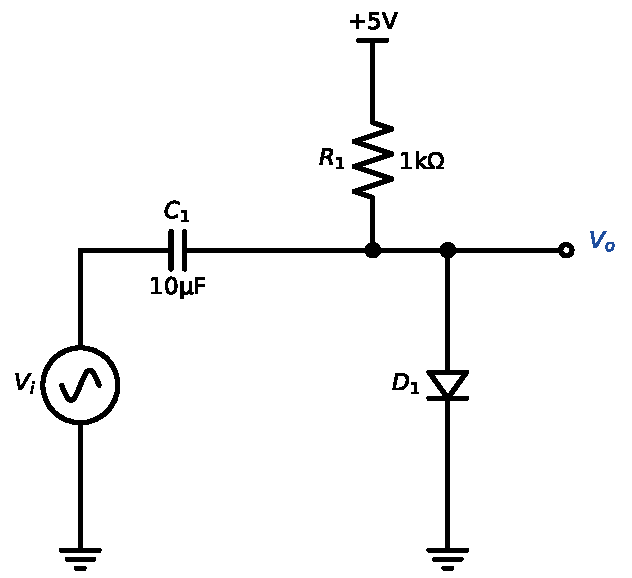
\includegraphics[width=\linewidth,height=5.6cm,keepaspectratio]{p01_circuit}\end{center}
\end{probbox}

\begin{probbox}{Problem 3D.2 \hfill Easy}
In the circuit below, $V_i(t) = 0.002\sin\left(2\pi\cdot 10000\,t\right)$. (a) Using the constant-voltage-drop model of the diode ($0.7$\,V), find the DC diode current $I_D$ and the DC output voltage $V_{o,dc}$. (b) Find the small-signal transfer function $\frac{V_o(s)}{V_i(s)}$ (use $n=1.8$, $V_T = 25$\,mV for $r_d$) and sketch its magnitude Bode plot. (c) Find the total output $V_o(t)$.
\begin{center}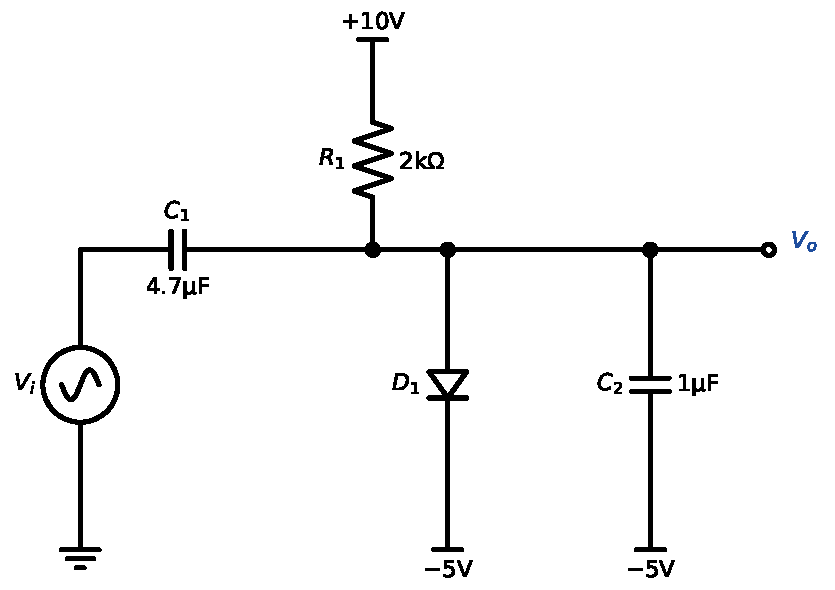
\includegraphics[width=\linewidth,height=5.6cm,keepaspectratio]{p02_circuit}\end{center}
\end{probbox}

\begin{probbox}{Problem 3D.3 \hfill Easy}
In the circuit below, $V_i(t) = 0.001\sin\left(2\pi\cdot 2000\,t\right)$. (a) Using the constant-voltage-drop model of the diode ($0.7$\,V), find the DC diode current $I_D$ and the DC output voltage $V_{o,dc}$. (b) Find the small-signal transfer function $\frac{V_o(s)}{V_i(s)}$ (use $n=1.8$, $V_T = 25$\,mV for $r_d$) and sketch its magnitude Bode plot. (c) Find the total output $V_o(t)$.
\begin{center}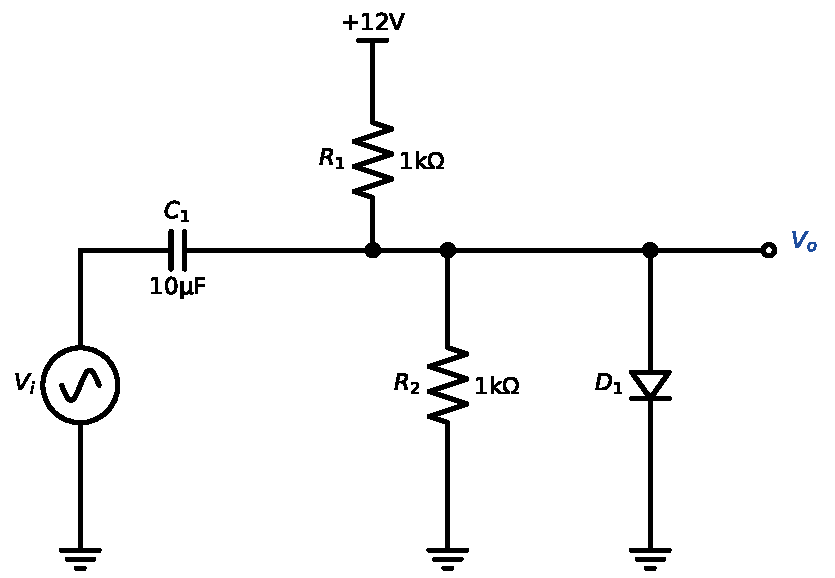
\includegraphics[width=\linewidth,height=5.6cm,keepaspectratio]{p03_circuit}\end{center}
\end{probbox}

\begin{probbox}{Problem 3D.4 \hfill Easy}
In the circuit below the op-amp is ideal and the input is $V_{DC} + v_i(t)$ with $V_{DC} = 0.5$\,V and $v_i(t) = 0.02\sin\left(2\pi\cdot 1000\,t\right)$. (a) Using the constant-voltage-drop model of the diode ($0.7$\,V), find the DC diode current $I_D$ and the DC output voltage $V_{o,dc}$. (b) Find the small-signal transfer function $\frac{V_o(s)}{V_i(s)}$ (use $n=1.8$, $V_T = 25$\,mV for $r_d$) and sketch its magnitude Bode plot. (c) Find the total output $V_o(t)$.
\begin{center}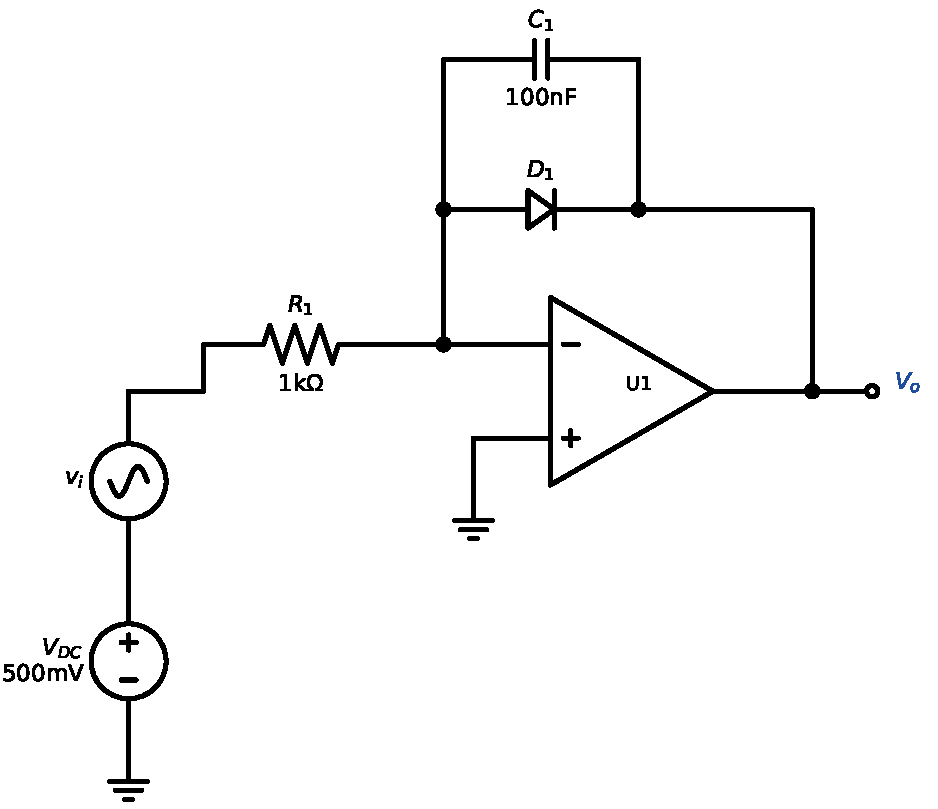
\includegraphics[width=\linewidth,height=5.6cm,keepaspectratio]{p04_circuit}\end{center}
\end{probbox}

\begin{probbox}{Problem 3D.5 \hfill Easy}
In the circuit below the op-amp is ideal and the input is $V_{DC} + v_i(t)$ with $V_{DC} = 0.55$\,V and $v_i(t) = 0.002\sin\left(2\pi\cdot 1000\,t\right)$. (a) Using the exponential model of the diode ($I_S = 2.6\times 10^{-9}$\,A, $n = 1.8$, $V_T = 25$\,mV), find the DC diode current $I_D$ and the DC output voltage $V_{o,dc}$. (b) Find the small-signal transfer function $\frac{V_o(s)}{V_i(s)}$ (use $n=1.8$, $V_T = 25$\,mV for $r_d$) and sketch its magnitude Bode plot. (c) Find the total output $V_o(t)$.
\begin{center}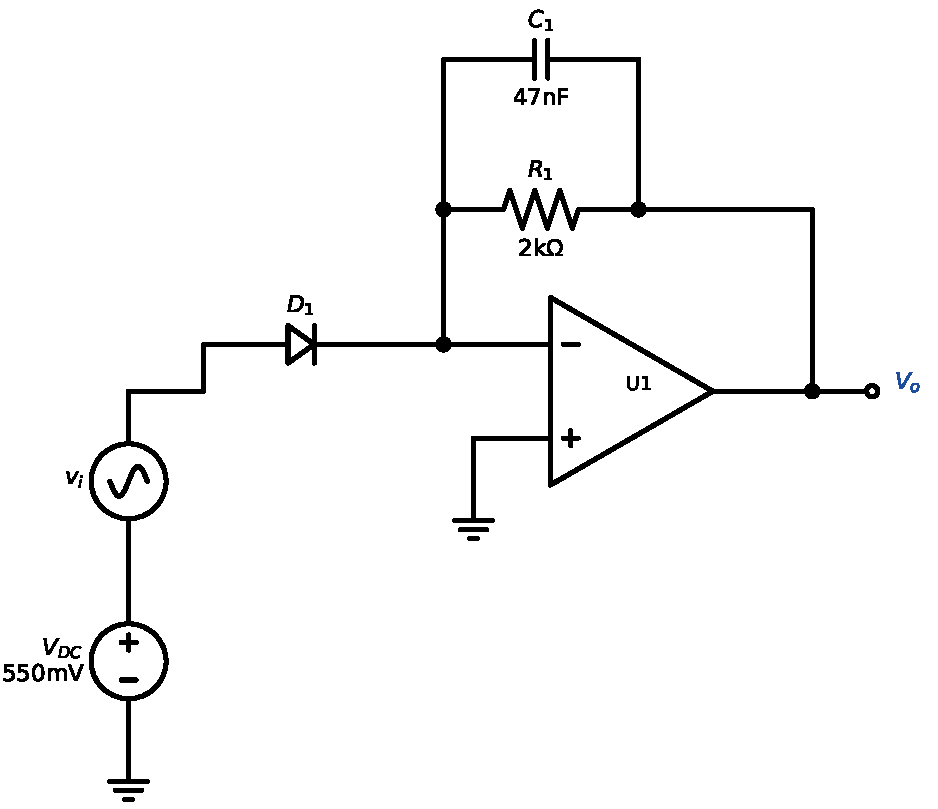
\includegraphics[width=\linewidth,height=5.6cm,keepaspectratio]{p05_circuit}\end{center}
\end{probbox}

\begin{probbox}{Problem 3D.6 \hfill Easy}
In the circuit below, $V_i(t) = 0.005\sin\left(2\pi\cdot 1000\,t\right)$. (a) Using the constant-voltage-drop model of the diode ($0.7$\,V), find the DC diode current $I_D$ and the DC output voltage $V_{o,dc}$. (b) Find the small-signal transfer function $\frac{V_o(s)}{V_i(s)}$ (use $n=1.8$, $V_T = 25$\,mV for $r_d$) and sketch its magnitude Bode plot. (c) Find the total output $V_o(t)$.
\begin{center}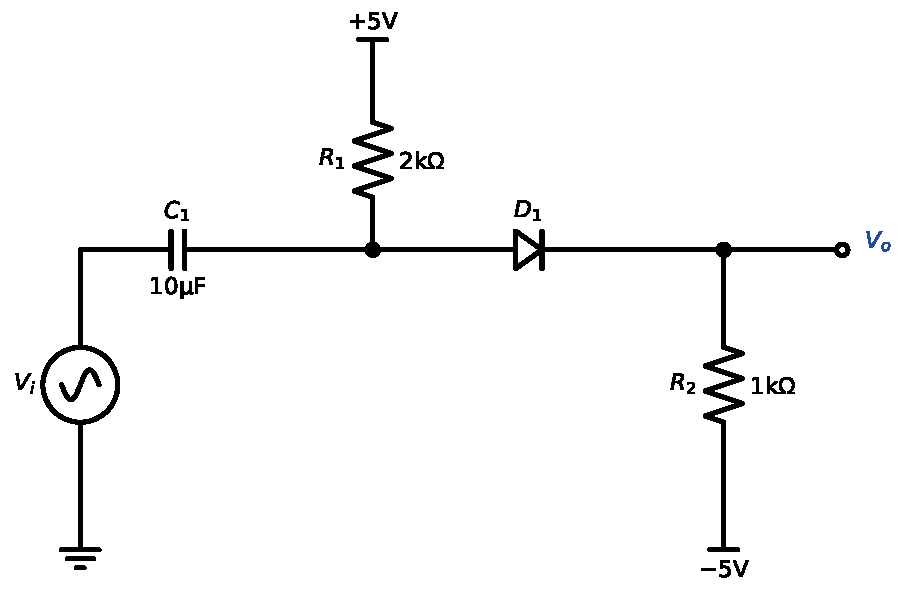
\includegraphics[width=\linewidth,height=5.6cm,keepaspectratio]{p06_circuit}\end{center}
\end{probbox}

\subsection*{Medium problems}
\begin{probbox}{Problem 3D.7 \hfill Medium}
In the circuit below, $V_i(t) = 0.002\sin\left(2\pi\cdot 10000\,t\right)$. (a) Using the constant-voltage-drop model of the diode ($0.7$\,V), find the DC diode current $I_D$ and the DC output voltage $V_{o,dc}$. (b) Find the small-signal transfer function $\frac{V_o(s)}{V_i(s)}$ (use $n=1.8$, $V_T = 25$\,mV for $r_d$) and sketch its magnitude Bode plot. (c) Find the total output $V_o(t)$.
\begin{center}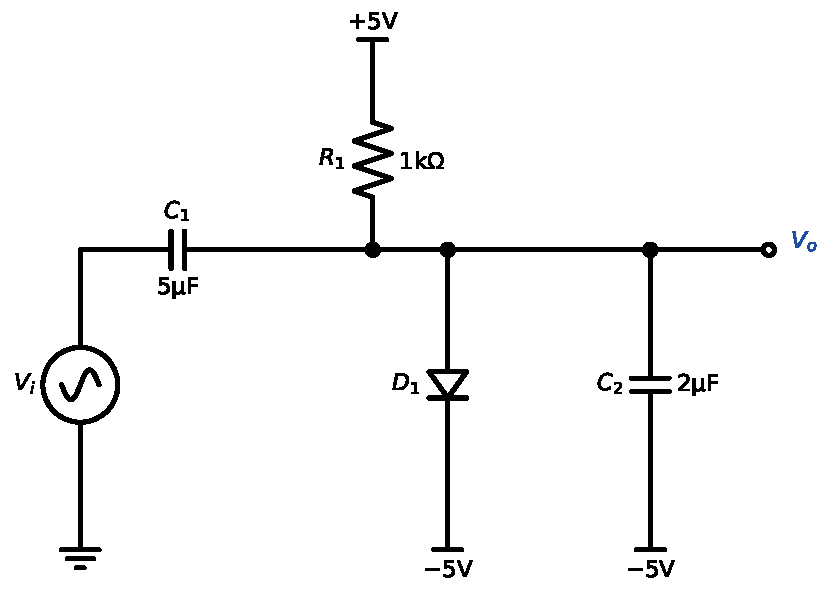
\includegraphics[width=\linewidth,height=5.6cm,keepaspectratio]{p07_circuit}\end{center}
\end{probbox}

\begin{probbox}{Problem 3D.8 \hfill Medium}
In the circuit below, $V_i(t) = 0.002\sin\left(2\pi\cdot 5000\,t\right)$. (a) Using the exponential model of the diode ($I_S = 2.6\times 10^{-9}$\,A, $n = 1.8$, $V_T = 25$\,mV), find the DC diode current $I_D$ and the DC output voltage $V_{o,dc}$. (b) Find the small-signal transfer function $\frac{V_o(s)}{V_i(s)}$ (use $n=1.8$, $V_T = 25$\,mV for $r_d$) and sketch its magnitude Bode plot. (c) Find the total output $V_o(t)$.
\begin{center}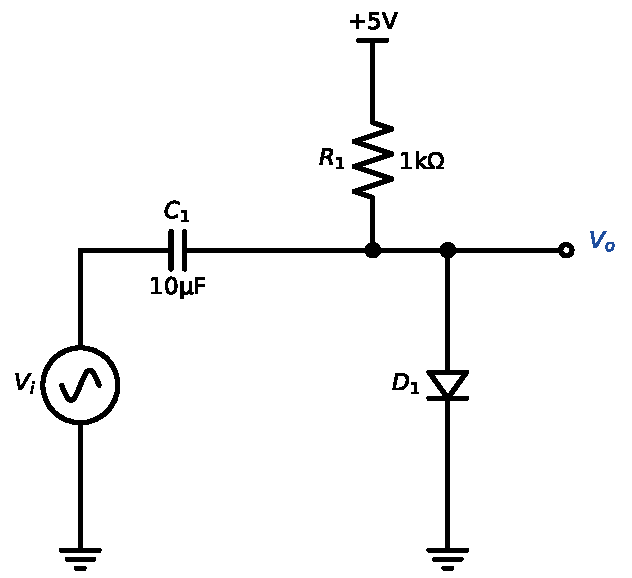
\includegraphics[width=\linewidth,height=5.6cm,keepaspectratio]{p08_circuit}\end{center}
\end{probbox}

\begin{probbox}{Problem 3D.9 \hfill Medium}
In the circuit below the op-amp is ideal and the input is $V_{DC} + v_i(t)$ with $V_{DC} = 0.5$\,V and $v_i(t) = 0.05\sin\left(2\pi\cdot 1000\,t\right)$. (a) Using the exponential model of the diode ($I_S = 2.6\times 10^{-9}$\,A, $n = 1.8$, $V_T = 25$\,mV), find the DC diode current $I_D$ and the DC output voltage $V_{o,dc}$. (b) Find the small-signal transfer function $\frac{V_o(s)}{V_i(s)}$ (use $n=1.8$, $V_T = 25$\,mV for $r_d$) and sketch its magnitude Bode plot. (c) Find the total output $V_o(t)$.
\begin{center}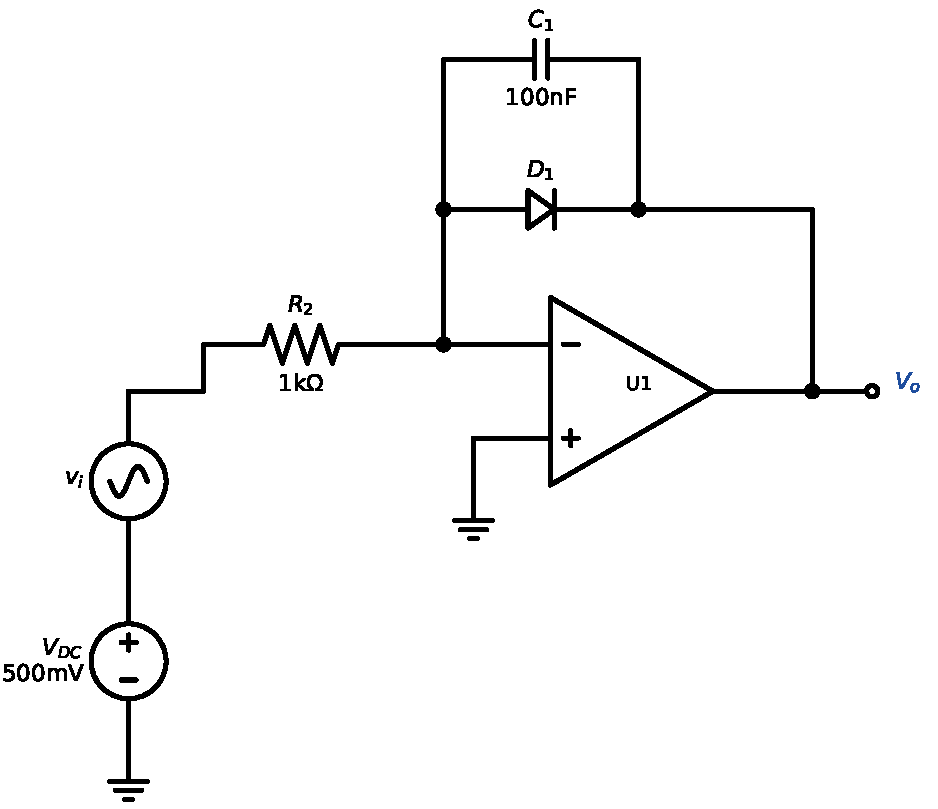
\includegraphics[width=\linewidth,height=5.6cm,keepaspectratio]{p09_circuit}\end{center}
\end{probbox}

\begin{probbox}{Problem 3D.10 \hfill Medium}
In the circuit below the op-amp is ideal and the input is $V_{DC} + v_i(t)$ with $V_{DC} = 0.6$\,V and $v_i(t) = 0.003\sin\left(2\pi\cdot 1000\,t\right)$. (a) Using the exponential model of the diode ($I_S = 2.6\times 10^{-9}$\,A, $n = 1.8$, $V_T = 25$\,mV), find the DC diode current $I_D$ and the DC output voltage $V_{o,dc}$. (b) Find the small-signal transfer function $\frac{V_o(s)}{V_i(s)}$ (use $n=1.8$, $V_T = 25$\,mV for $r_d$) and sketch its magnitude Bode plot. (c) Find the total output $V_o(t)$.
\begin{center}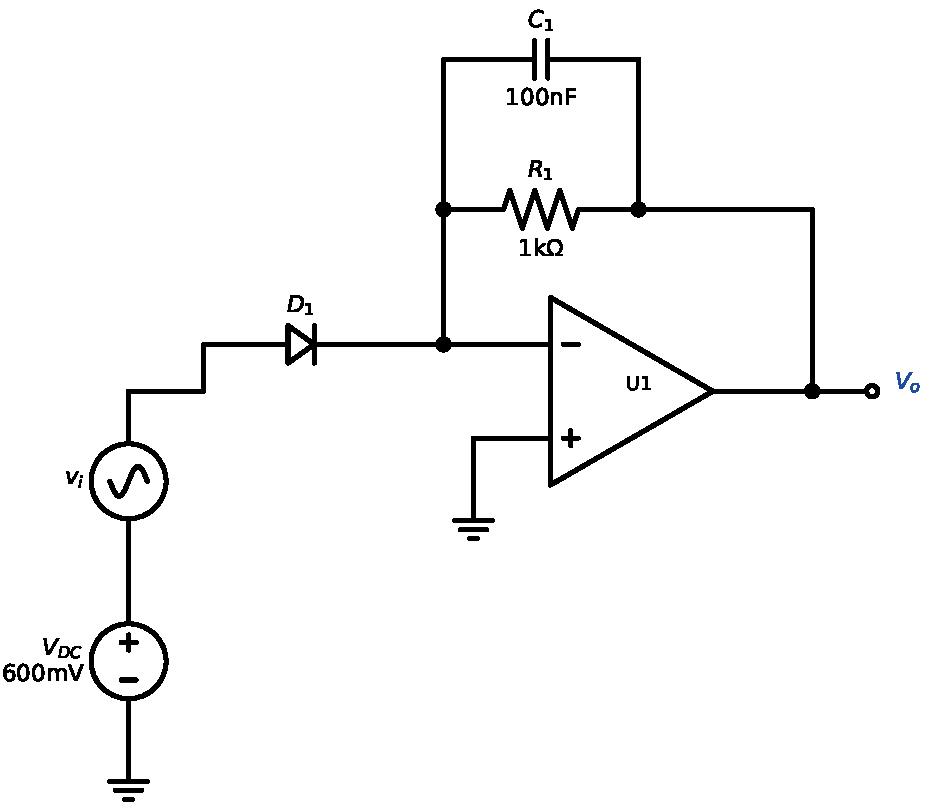
\includegraphics[width=\linewidth,height=5.6cm,keepaspectratio]{p10_circuit}\end{center}
\end{probbox}

\begin{probbox}{Problem 3D.11 \hfill Medium}
In the circuit below the op-amp is ideal and the input is $V_{DC} + v_i(t)$ with $V_{DC} = 1$\,V and $v_i(t) = 0.05\sin\left(2\pi\cdot 2000\,t\right)$. (a) Using the constant-voltage-drop model of the diode ($0.7$\,V), find the DC diode current $I_D$ and the DC output voltage $V_{o,dc}$. (b) Find the small-signal transfer function $\frac{V_o(s)}{V_i(s)}$ (use $n=1.8$, $V_T = 25$\,mV for $r_d$) and sketch its magnitude Bode plot. (c) Find the total output $V_o(t)$.
\begin{center}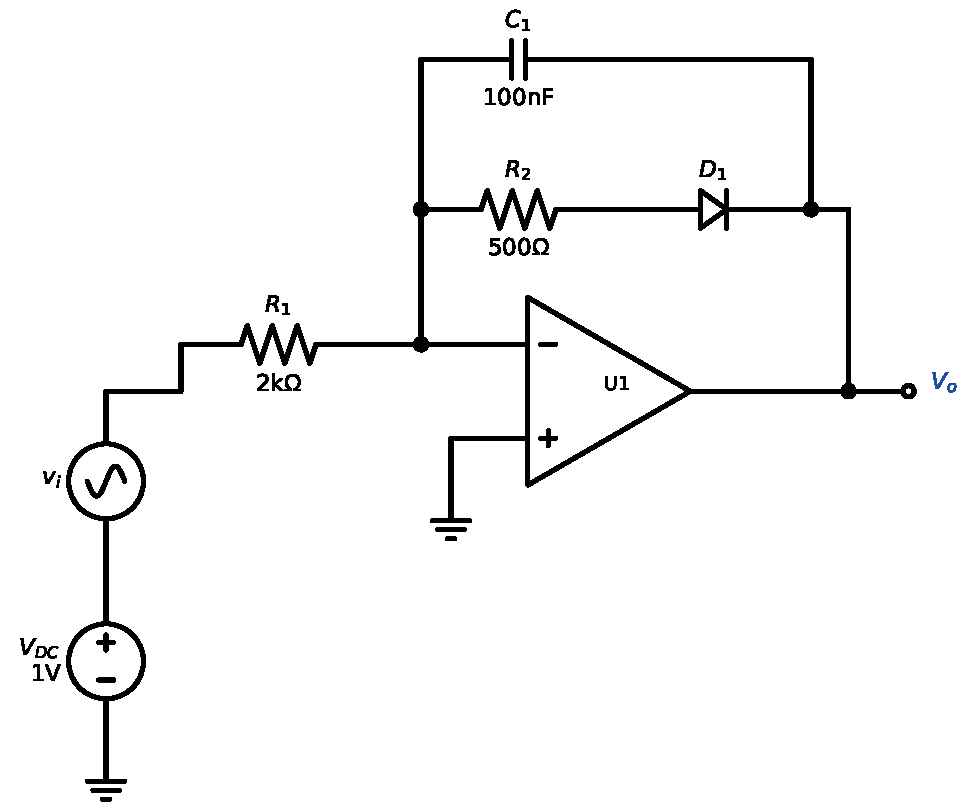
\includegraphics[width=\linewidth,height=5.6cm,keepaspectratio]{p11_circuit}\end{center}
\end{probbox}

\begin{probbox}{Problem 3D.12 \hfill Medium}
In the circuit below, $V_i(t) = 0.002\sin\left(2\pi\cdot 1000\,t\right)$. (a) Using the constant-voltage-drop model of the diode ($0.7$\,V), find the DC diode current $I_D$ and the DC output voltage $V_{o,dc}$. (b) Find the small-signal transfer function $\frac{V_o(s)}{V_i(s)}$ (use $n=1.8$, $V_T = 25$\,mV for $r_d$) and sketch its magnitude Bode plot. (c) Find the total output $V_o(t)$.
\begin{center}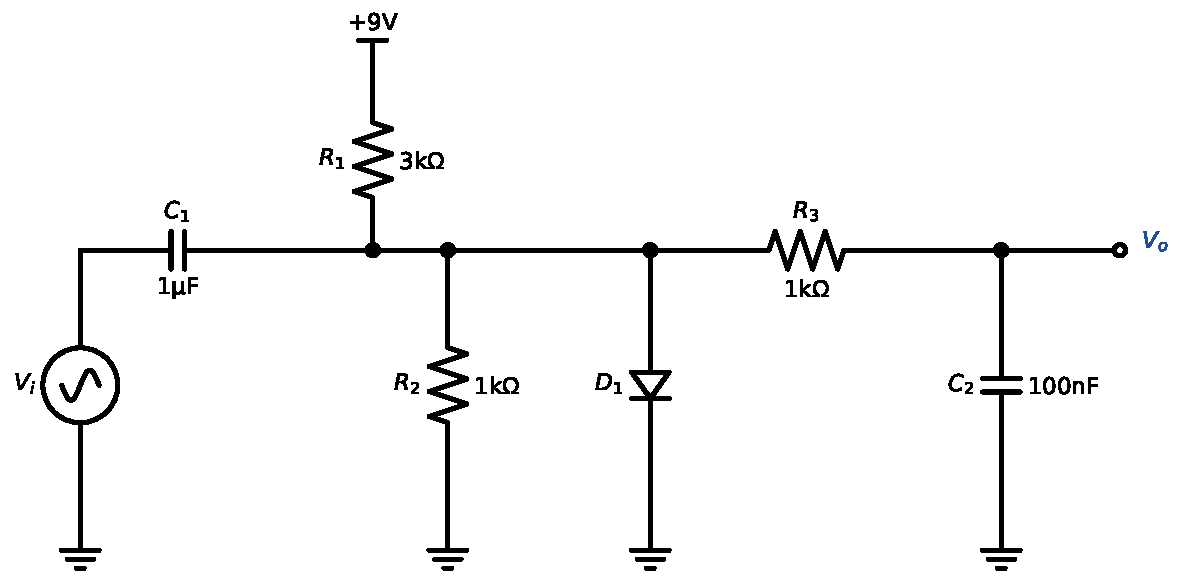
\includegraphics[width=\linewidth,height=5.6cm,keepaspectratio]{p12_circuit}\end{center}
\end{probbox}

\subsection*{Hard problems}
\begin{probbox}{Problem 3D.13 \hfill Hard}
In the circuit below, $V_i(t) = 0.003\sin\left(2\pi\cdot 2000\,t\right)$. (a) Using the exponential model of the diode ($I_S = 10^{-12}$\,A, $n = 1$, $V_T = 25$\,mV), find the DC diode current $I_D$ and the DC output voltage $V_{o,dc}$. (b) Find the small-signal transfer function $\frac{V_o(s)}{V_i(s)}$ (use $n=1$, $V_T = 25$\,mV for $r_d$) and sketch its magnitude Bode plot. (c) Find the total output $V_o(t)$.
\begin{center}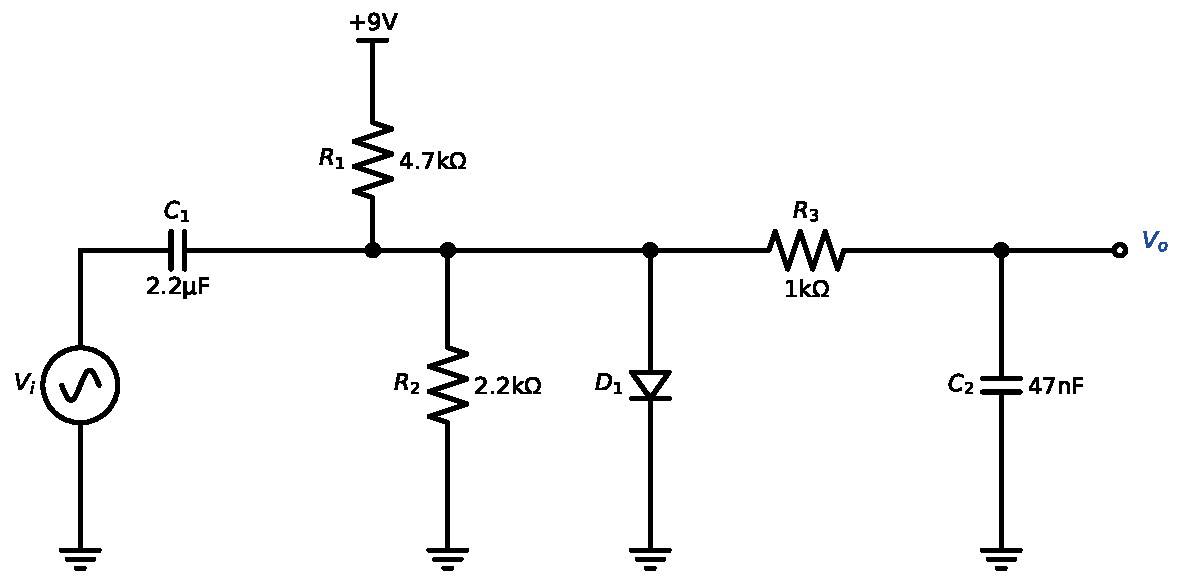
\includegraphics[width=\linewidth,height=5.6cm,keepaspectratio]{p13_circuit}\end{center}
\end{probbox}

\begin{probbox}{Problem 3D.14 \hfill Hard}
In the circuit below the op-amp is ideal and the input is $V_{DC} + v_i(t)$ with $V_{DC} = 1$\,V and $v_i(t) = 0.01\sin\left(2\pi\cdot 3000\,t+\frac{\pi}{4}\right)$. (a) Using the exponential model of the diode ($I_S = 2.6\times 10^{-9}$\,A, $n = 1.8$, $V_T = 25$\,mV), find the DC diode current $I_D$ and the DC output voltage $V_{o,dc}$. (b) Find the small-signal transfer function $\frac{V_o(s)}{V_i(s)}$ (use $n=1.8$, $V_T = 25$\,mV for $r_d$) and sketch its magnitude Bode plot. (c) Find the total output $V_o(t)$.
\begin{center}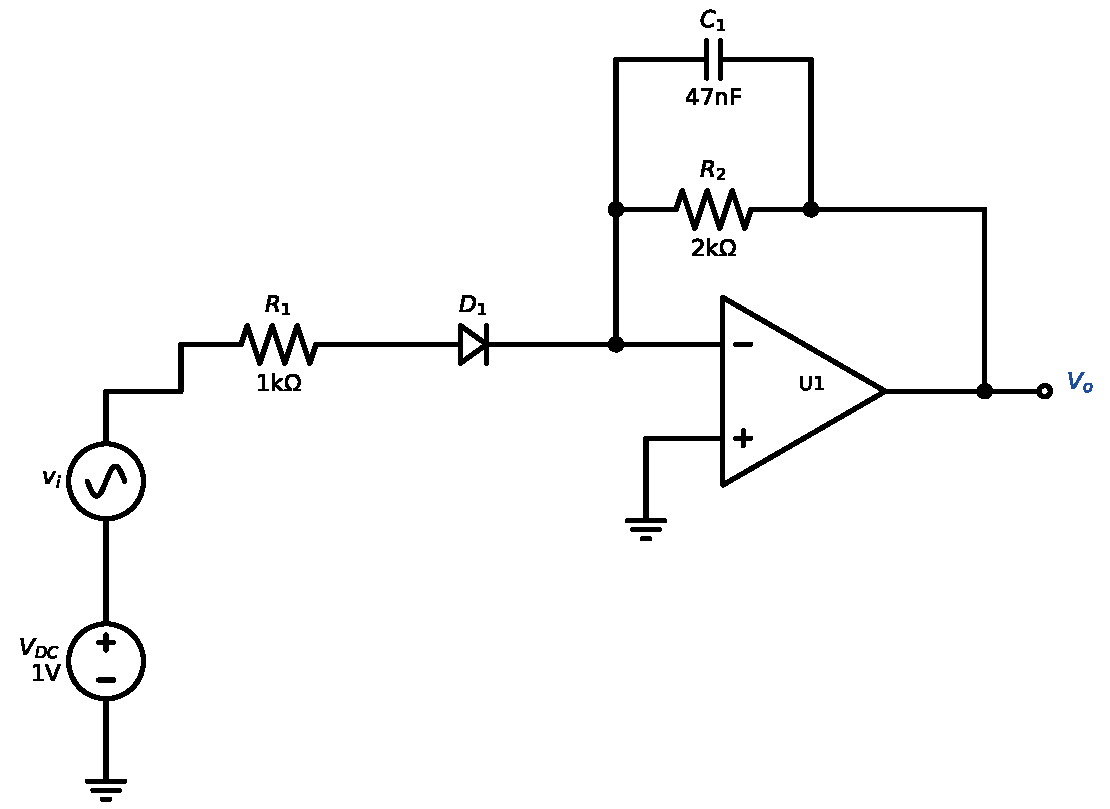
\includegraphics[width=\linewidth,height=5.6cm,keepaspectratio]{p14_circuit}\end{center}
\end{probbox}

\begin{probbox}{Problem 3D.15 \hfill Hard}
In the circuit below, $V_i(t) = 0.002\sin\left(2\pi\cdot 1000\,t\right)$. (a) Using the constant-voltage-drop model of the diode ($0.7$\,V), find the DC diode current $I_D$ and the DC output voltage $V_{o,dc}$. (b) Find the small-signal transfer function $\frac{V_o(s)}{V_i(s)}$ (use $n=1.8$, $V_T = 25$\,mV for $r_d$) and sketch its magnitude Bode plot. (c) Find the total output $V_o(t)$.
\begin{center}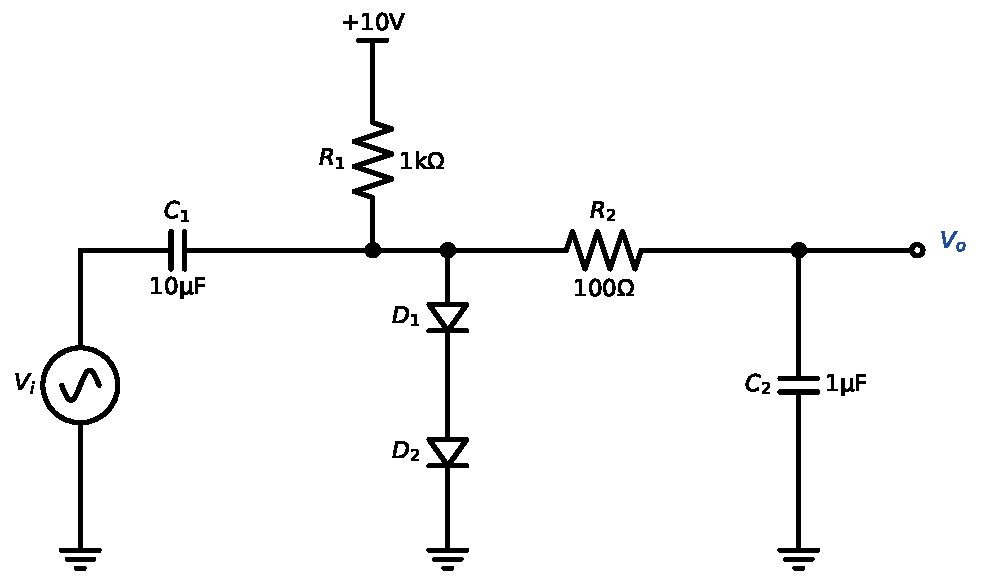
\includegraphics[width=\linewidth,height=5.6cm,keepaspectratio]{p15_circuit}\end{center}
\end{probbox}

\begin{probbox}{Problem 3D.16 \hfill Hard}
In the circuit below the op-amp is ideal and the input is $V_{DC} + v_i(t)$ with $V_{DC} = 1$\,V and $v_i(t) = 0.02\sin\left(2\pi\cdot 2000\,t\right)$. (a) Using the exponential model of the diode ($I_S = 2.6\times 10^{-9}$\,A, $n = 1.8$, $V_T = 25$\,mV), find the DC diode current $I_D$ and the DC output voltage $V_{o,dc}$. (b) Find the small-signal transfer function $\frac{V_o(s)}{V_i(s)}$ (use $n=1.8$, $V_T = 25$\,mV for $r_d$) and sketch its magnitude Bode plot. (c) Find the total output $V_o(t)$.
\begin{center}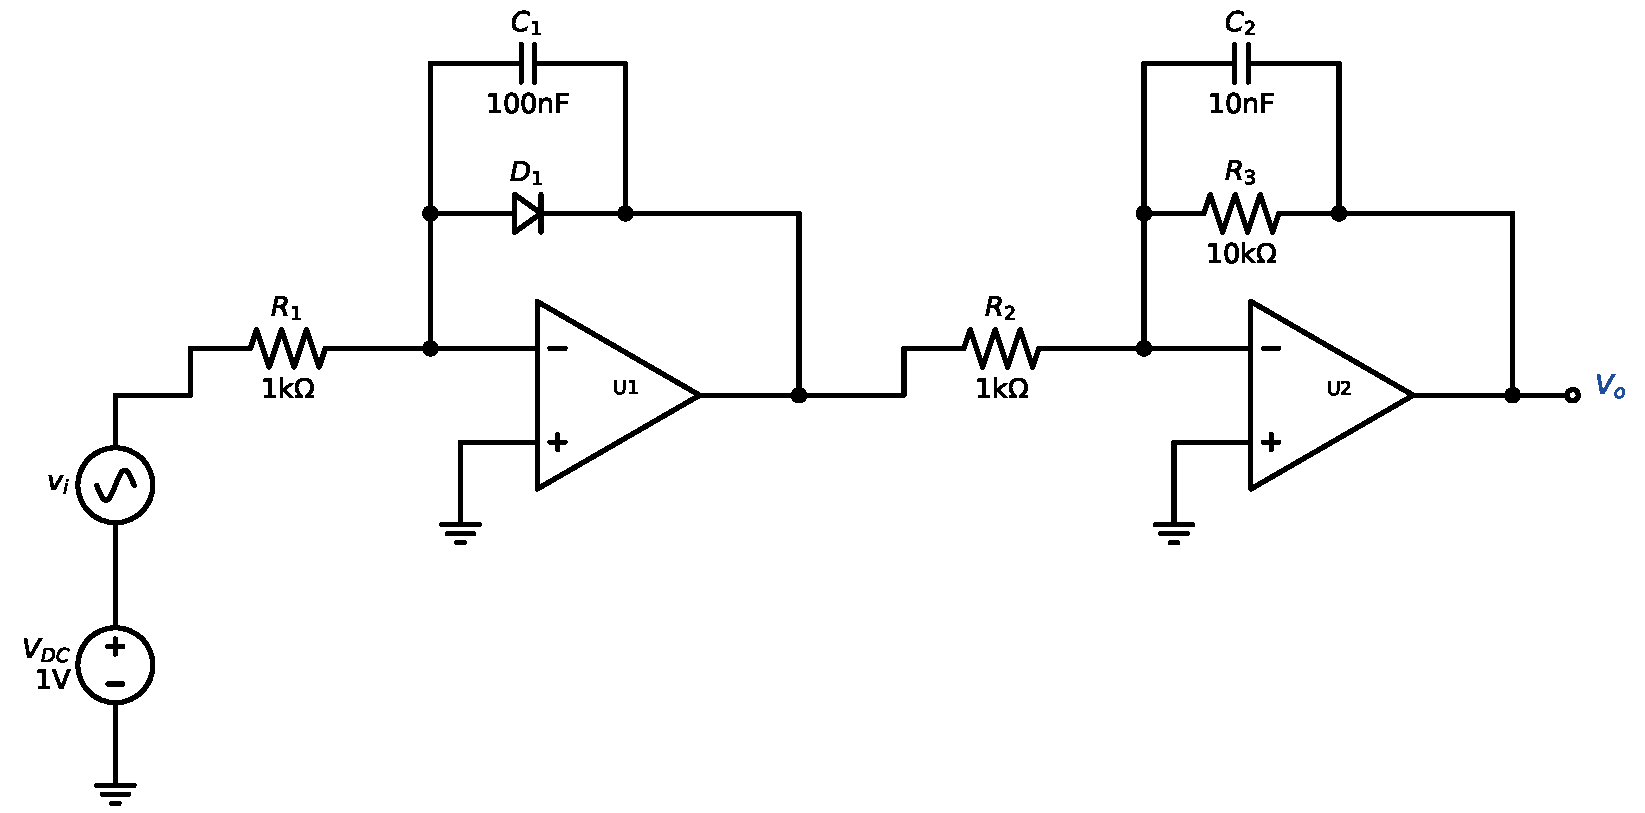
\includegraphics[width=\linewidth,height=5.6cm,keepaspectratio]{p16_circuit}\end{center}
\end{probbox}

\begin{probbox}{Problem 3D.17 \hfill Hard}
In the circuit below, $V_i(t) = 0.005\sin\left(2\pi\cdot 500\,t\right)$. (a) Using the exponential model of the diode ($I_S = 2.6\times 10^{-9}$\,A, $n = 1.8$, $V_T = 25$\,mV), find the DC diode current $I_D$ and the DC output voltage $V_{o,dc}$. (b) Find the small-signal transfer function $\frac{V_o(s)}{V_i(s)}$ (use $n=1.8$, $V_T = 25$\,mV for $r_d$) and sketch its magnitude Bode plot. (c) Find the total output $V_o(t)$.
\begin{center}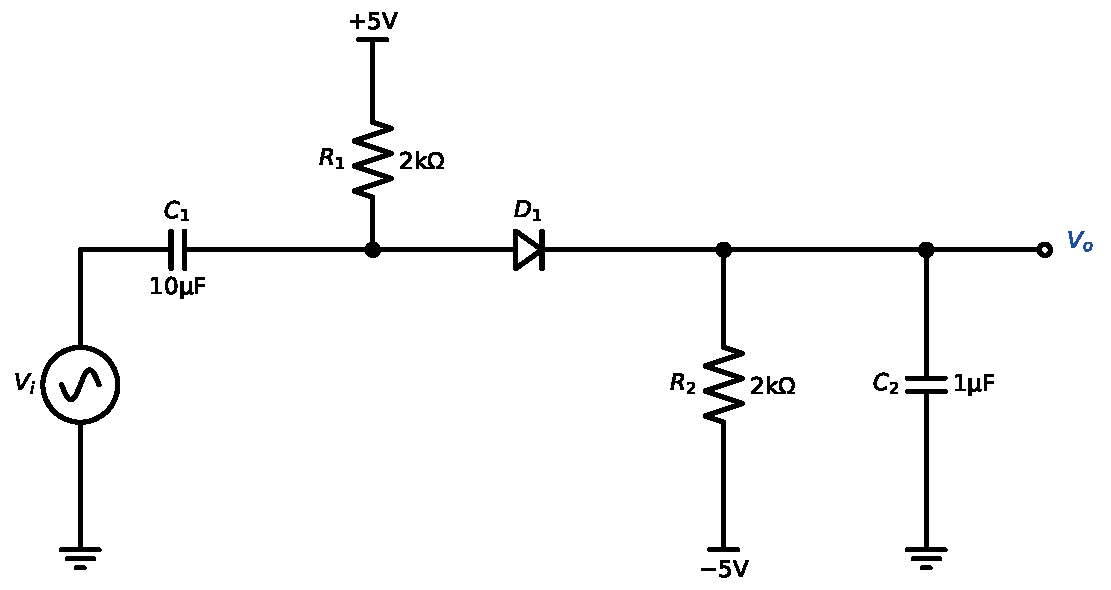
\includegraphics[width=\linewidth,height=5.6cm,keepaspectratio]{p17_circuit}\end{center}
\end{probbox}

\begin{probbox}{Problem 3D.18 \hfill Hard}
In the circuit below the op-amp is ideal and the input is $V_{DC} + v_i(t)$ with $V_{DC} = 0.8$\,V and $v_i(t) = 0.005\cos\left(2\pi\cdot 500\,t-\frac{\pi}{3}\right)$. (a) Using the exponential model of the diode ($I_S = 10^{-12}$\,A, $n = 1$, $V_T = 25$\,mV), find the DC diode current $I_D$ and the DC output voltage $V_{o,dc}$. (b) Find the small-signal transfer function $\frac{V_o(s)}{V_i(s)}$ (use $n=1$, $V_T = 25$\,mV for $r_d$) and sketch its magnitude Bode plot. (c) Find the total output $V_o(t)$.
\begin{center}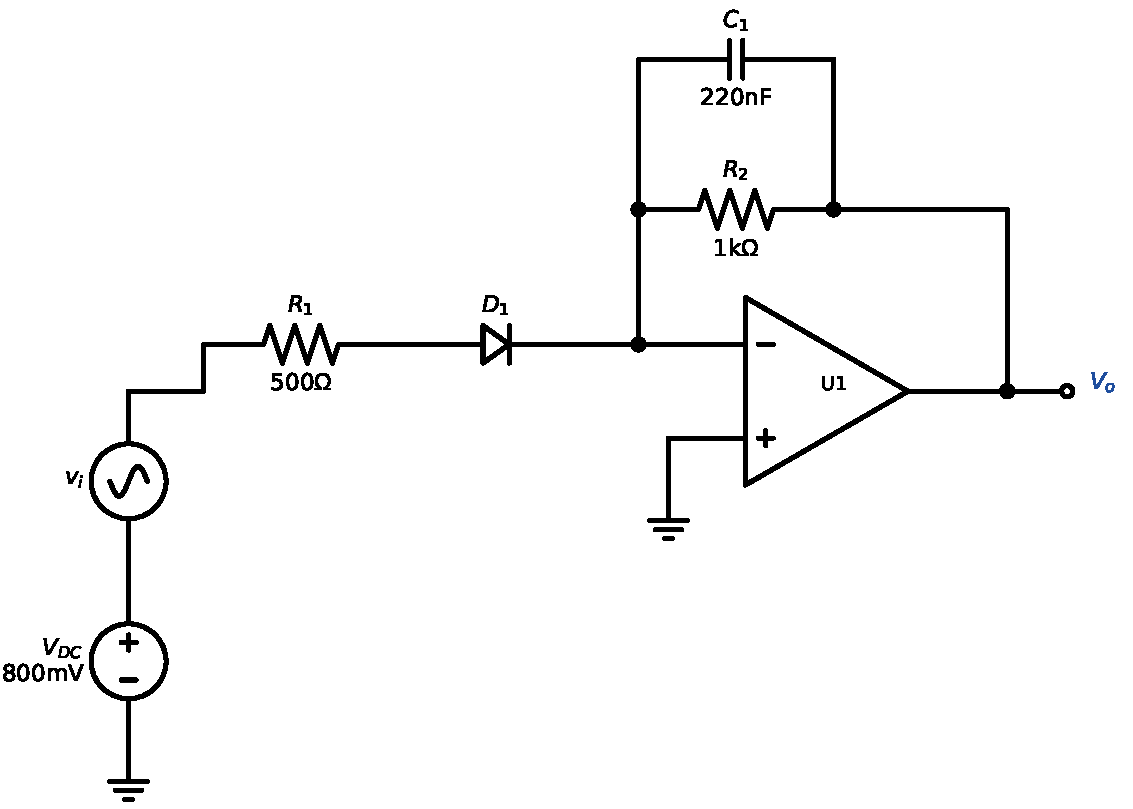
\includegraphics[width=\linewidth,height=5.6cm,keepaspectratio]{p18_circuit}\end{center}
\end{probbox}

\newpage
\section*{Solutions}
Every solution follows the steps of the Lecture-3 pipeline card.
\newpage
\subsection*{Solution 3D.1 \hfill Easy}
\begin{center}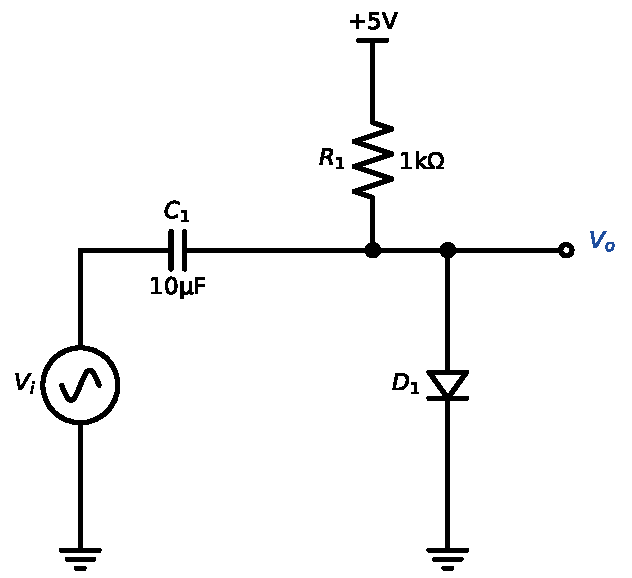
\includegraphics[width=0.9\linewidth,height=5cm,keepaspectratio]{p01_circuit}\end{center}
\solstep{1}{DC operating point}DC rules (tool T3): $v_i = 0$ and every capacitor is open ($C_{1}$). Assume the diode is ON (constant-voltage-drop model, $0.7$\,V) and solve the DC circuit:

Replace $D_{1}$ ON: a $0.7$\,V source ($V_{o} - 0 = 0.7$) carrying an unknown current $I_{D_{1}}$ from anode to cathode.

Equations (KCL at every node that is not an op-amp output, plus the diode voltages):\begin{align*}
&\text{KCL at }V_{o}: && \frac{V_{o} - 5}{R_{1}} + I_{D_{1}} = 0 \\
&\text{D1 ON}: && V_{o} - 0 = 0.7
\end{align*}


Solving these linear equations (substitute one into the other, as in Lecture 2) gives, with $V_i$ kept as a symbol:\begin{align*}
V_{o} &= 0.7 \\
I_{D_{1}} &= 4.3\ \mathrm{mA}
\end{align*}


 $I_{D_{1}} = 4.3\,\mathrm{m}\mathrm{A} > 0$ \checkmark, so the assumption holds.\[
\boxed{V_{o,dc} = 700\,\mathrm{m}\mathrm{V}}
\]

\solstep{2}{Small-signal resistance}$r_{d} = \frac{nV_T}{I_D} = \frac{1.8\times 25\,\mathrm{mV}}{4.3\,\mathrm{m}\mathrm{A}} = 10.5\,\Omega$ (tool T3). For the AC analysis the diode is just this resistor.
\solstep{3}{AC circuit}Set every DC supply to zero: each supply rail becomes AC ground. Replace every capacitor by $\frac{1}{sC}$ and every inductor by $sL$.
AC equivalent circuit (nodes named for the next step):
\begin{center}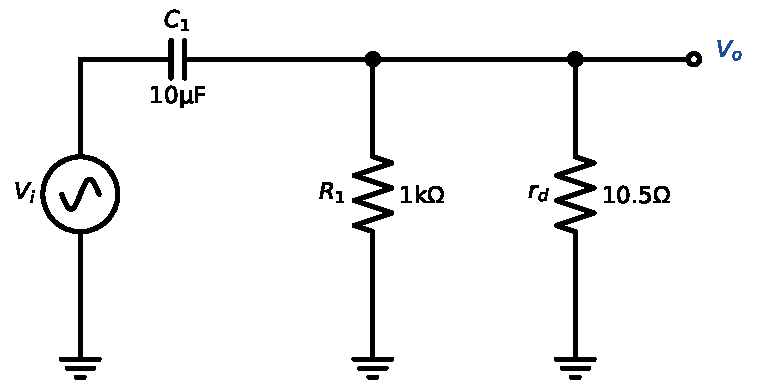
\includegraphics[width=0.95\linewidth,height=5.2cm,keepaspectratio]{p01_ac}\end{center}

\solstep{4}{Transfer function by a chain of dividers}Walk from the input to the output through the named nodes: $V_{i} \to V_{o}$. There is a single link, so $H(s)$ is just one voltage divider (tool T2).
Impedances seen \emph{looking right} from a node (everything from that node to ground, excluding what is on its left). Compute them from the far right toward the input:
\begin{align*}
Z_{o} &= R_{1} \parallel r_d = 10.4
\end{align*}

Now each link. {\small (Algebra tip: to simplify a fraction that contains fractions, multiply its top and bottom by every inner denominator; then divide top and bottom by the leading coefficient of the denominator so that it starts with a plain $s^n$.)}
\begin{align*}
\frac{V_{o}}{V_{i}} &= \frac{Z_{o}}{\frac{1}{sC_{1}} + Z_{o}} = \dfrac{s}{s + 9660}
\end{align*}
So:\[
H(s) = \dfrac{s}{s + 9660}
\]

\solstep{5}{Standard (Bode-ready) form}Find the roots. Every root $s=-p$ of the denominator is a \emph{pole}, every root $s=-z$ of the numerator is a \emph{zero}; $|p|$ and $|z|$ are the corner frequencies (rad/s).
\begin{itemize}[leftmargin=*,itemsep=2pt]
\item Numerator: it has the factor $s$ $\Rightarrow$ 1 zero at $s=0$.
\item Denominator: $s + 9660$; $s + 9660 = 0 \Rightarrow s = -9660$.
\end{itemize}

Factored form (leading coefficient in front):
\[
H(s) = 1\,\dfrac{s}{(s+9660)}
\]

Bode-ready form: rewrite every $(s+p) = p\left(1+\frac{s}{p}\right)$ and $(s+z) = z\left(1+\frac{s}{z}\right)$, and collect all constants into $K$. Each $s$ in the numerator is paired with one of the \emph{lowest} poles as $\frac{s}{s+p}$ (that factor is $\approx 1$ above $p$). Then every factor except $K$ is $\approx 1$ inside the pass-band:
\[
H(s) = 1\,\dfrac{s}{s+2\pi\cdot 1.54\mathrm{k}},\qquad K = 1
\]

\begin{center}\renewcommand{\arraystretch}{1.35}
\begin{tabular}{cccc}
\toprule
type & $\omega_c$ (rad/s) & $f_c=\omega_c/2\pi$ & slope change \\
\midrule
pole & $9660$ & 1.54 kHz & $-20$ dB/dec \\
\bottomrule
\end{tabular}\end{center}

\solstep{6}{Magnitude Bode plot}Below every corner $|H(s)|\approx 1.04\times 10^{-4}\,s$, so the plot starts with a slope of $+20$\,dB/dec. Then, moving right, each pole bends the line down by 20\,dB/dec and each zero bends it up by 20\,dB/dec (tool T6):
\begin{center}\renewcommand{\arraystretch}{1.35}
\begin{tabular}{lcl}
\toprule
frequency range & slope & asymptote level \\
\midrule
$f<$ 1.54 kHz & $+20$ dB/dec & 0 dB at end \\
$f>$ 1.54 kHz & $0$ dB/dec (flat) & 0 dB at start \\
\bottomrule
\end{tabular}\end{center}

The flat (pass-band) level is $20\log_{10}|K| = 20\log_{10}1 = 0$\,dB.
\begin{center}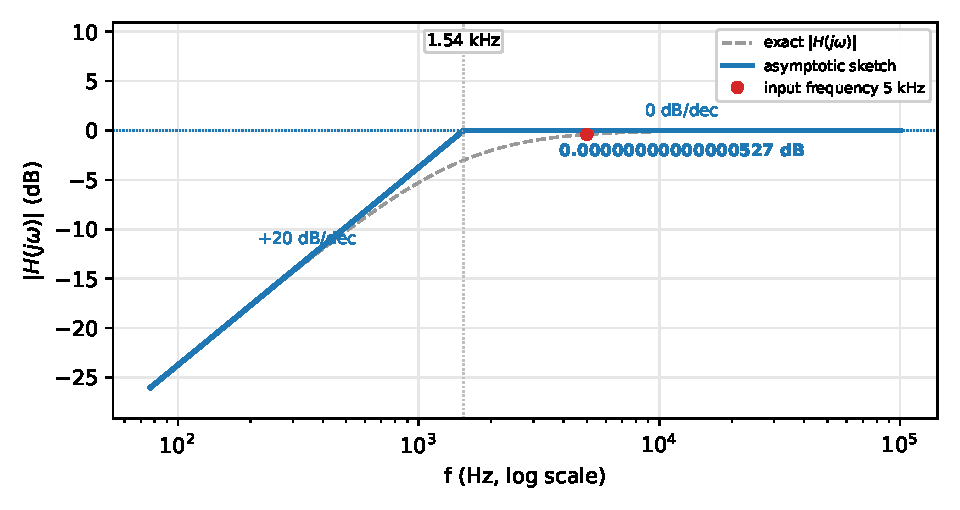
\includegraphics[width=0.78\linewidth,height=6.5cm,keepaspectratio]{p01_bode}\end{center}

{\small Blue: the straight-line sketch you are expected to draw. Dashed grey: the exact curve (about 3\,dB below the corner of an isolated pole). Red dot: the input frequency of Step 7.}
\solstep{7}{Total output (DC + AC)}The input is $V_i(t) = 0.002\sin\left(2\pi\cdot 5000\,t\right)$, so $\omega_{in} = 2\pi\cdot 5000 = 31400$\,rad/s. Put $s=j\omega_{in}$ in each factor (tool T5): magnitudes multiply, angles add.
{\small Rules: $\left|\frac{s}{s+p}\right| = \frac{\omega}{\sqrt{\omega^2+p^2}}$, $\angle = \frac{\pi}{2}-\tan^{-1}\frac{\omega}{p}$;\quad $\left|\frac{1}{1+s/p}\right| = \frac{1}{\sqrt{1+(\omega/p)^2}}$, $\angle = -\tan^{-1}\frac{\omega}{p}$;\quad $\left|1+\frac{s}{z}\right| = \sqrt{1+(\omega/z)^2}$, $\angle = \tan^{-1}\frac{\omega}{z}$;\quad a negative $K$ adds $-\pi$.}
\begin{center}\renewcommand{\arraystretch}{1.35}
\begin{tabular}{ccc}
\toprule
factor & magnitude & angle (rad) \\
\midrule
$1$ & $1$ & $0$ \\
$\rule[-1.1em]{0pt}{2.8em}\dfrac{s}{s+2\pi\cdot 1.54\mathrm{k}}$ & $0.9559$ & $0.298$ \\
\textbf{total} & $\mathbf{0.9559}$ (product) & $\mathbf{0.298}$ (sum) \\
\bottomrule
\end{tabular}\end{center}

\begin{align*}
|H(j\omega_{in})| &= 0.956, \qquad \angle H(j\omega_{in}) = 0.298\ \mathrm{rad} \\
v_{o,ac}(t) &= 0.956\times 0.002\,\sin\left(2\pi\cdot 5000\,t + 0.298\right) = 0.00191\,\sin\left(2\pi\cdot 5000\,t + 0.298\right)
\end{align*}

Add the DC part from Step 2 (superposition):
\[
\boxed{V_o(t) = 0.7 + 0.00191\,\sin\left(2\pi\cdot 5000\,t + 0.298\right)\ \mathrm{V}}
\]
 Check the small-signal assumption: the AC voltage across the diode has amplitude about $1.91\,\mathrm{m}\mathrm{V}$, well below $nV_T = 45\,\mathrm{m}\mathrm{V}$ \checkmark.
\begin{ansbox}
$H(s) = 1\,\dfrac{s}{s+2\pi\cdot 1.54\mathrm{k}}$\quad (corners: 1.54 kHz)\\[4pt]
$V_o(t) = 0.7 + 0.00191\,\sin\left(2\pi\cdot 5000\,t + 0.298\right)\ \mathrm{V}$
\end{ansbox}

\newpage
\subsection*{Solution 3D.2 \hfill Easy}
\begin{center}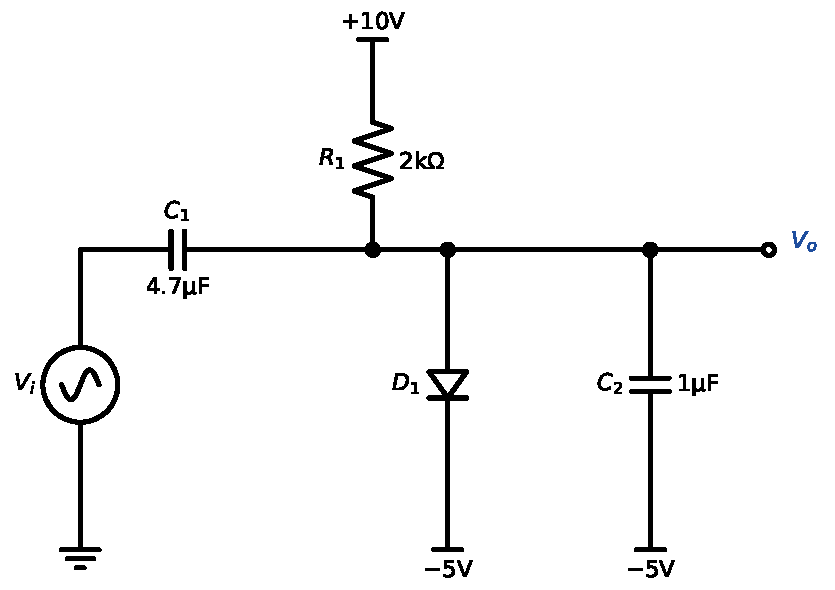
\includegraphics[width=0.9\linewidth,height=5cm,keepaspectratio]{p02_circuit}\end{center}
\solstep{1}{DC operating point}DC rules (tool T3): $v_i = 0$ and every capacitor is open ($C_{1}, C_{2}$). Assume the diode is ON (constant-voltage-drop model, $0.7$\,V) and solve the DC circuit:

Replace $D_{1}$ ON: a $0.7$\,V source ($V_{o} - -5 = 0.7$) carrying an unknown current $I_{D_{1}}$ from anode to cathode.

Equations (KCL at every node that is not an op-amp output, plus the diode voltages):\begin{align*}
&\text{KCL at }V_{o}: && \frac{V_{o} - 10}{R_{1}} + I_{D_{1}} = 0 \\
&\text{D1 ON}: && V_{o} - -5 = 0.7
\end{align*}


Solving these linear equations (substitute one into the other, as in Lecture 2) gives, with $V_i$ kept as a symbol:\begin{align*}
V_{o} &= -4.3 \\
I_{D_{1}} &= 7.15\ \mathrm{mA}
\end{align*}


 $I_{D_{1}} = 7.15\,\mathrm{m}\mathrm{A} > 0$ \checkmark, so the assumption holds.\[
\boxed{V_{o,dc} = -4.3\,\mathrm{V}}
\]

\solstep{2}{Small-signal resistance}$r_{d} = \frac{nV_T}{I_D} = \frac{1.8\times 25\,\mathrm{mV}}{7.15\,\mathrm{m}\mathrm{A}} = 6.29\,\Omega$ (tool T3). For the AC analysis the diode is just this resistor.
\solstep{3}{AC circuit}Set every DC supply to zero: each supply rail becomes AC ground. Replace every capacitor by $\frac{1}{sC}$ and every inductor by $sL$.
AC equivalent circuit (nodes named for the next step):
\begin{center}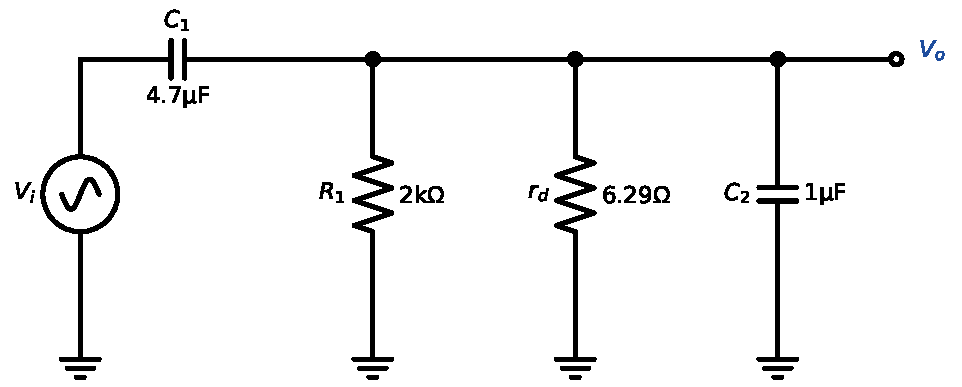
\includegraphics[width=0.95\linewidth,height=5.2cm,keepaspectratio]{p02_ac}\end{center}

\solstep{4}{Transfer function by a chain of dividers}Walk from the input to the output through the named nodes: $V_{i} \to V_{o}$. There is a single link, so $H(s)$ is just one voltage divider (tool T2).
Impedances seen \emph{looking right} from a node (everything from that node to ground, excluding what is on its left). Compute them from the far right toward the input:
\begin{align*}
Z_{o} &= R_{1} \parallel r_d \parallel \frac{1}{sC_{2}} = \dfrac{10^{6}}{s + 1.59\times 10^{5}}
\end{align*}

Now each link. {\small (Algebra tip: to simplify a fraction that contains fractions, multiply its top and bottom by every inner denominator; then divide top and bottom by the leading coefficient of the denominator so that it starts with a plain $s^n$.)}
\begin{align*}
\frac{V_{o}}{V_{i}} &= \frac{Z_{o}}{\frac{1}{sC_{1}} + Z_{o}} = \dfrac{0.825\,s}{s + 28000}
\end{align*}
So:\[
H(s) = \dfrac{0.825\,s}{s + 28000}
\]

\solstep{5}{Standard (Bode-ready) form}Find the roots. Every root $s=-p$ of the denominator is a \emph{pole}, every root $s=-z$ of the numerator is a \emph{zero}; $|p|$ and $|z|$ are the corner frequencies (rad/s).
\begin{itemize}[leftmargin=*,itemsep=2pt]
\item Numerator: it has the factor $s$ $\Rightarrow$ 1 zero at $s=0$.
\item Denominator: $s + 28000$; $s + 28000 = 0 \Rightarrow s = -28000$.
\end{itemize}

Factored form (leading coefficient in front):
\[
H(s) = 0.825\,\dfrac{s}{(s+28000)}
\]

Bode-ready form: rewrite every $(s+p) = p\left(1+\frac{s}{p}\right)$ and $(s+z) = z\left(1+\frac{s}{z}\right)$, and collect all constants into $K$. Each $s$ in the numerator is paired with one of the \emph{lowest} poles as $\frac{s}{s+p}$ (that factor is $\approx 1$ above $p$). Then every factor except $K$ is $\approx 1$ inside the pass-band:
\[
H(s) = 0.825\,\dfrac{s}{s+2\pi\cdot 4.45\mathrm{k}},\qquad K = 0.825
\]

\begin{center}\renewcommand{\arraystretch}{1.35}
\begin{tabular}{cccc}
\toprule
type & $\omega_c$ (rad/s) & $f_c=\omega_c/2\pi$ & slope change \\
\midrule
pole & $28000$ & 4.45 kHz & $-20$ dB/dec \\
\bottomrule
\end{tabular}\end{center}

\solstep{6}{Magnitude Bode plot}Below every corner $|H(s)|\approx 2.95\times 10^{-5}\,s$, so the plot starts with a slope of $+20$\,dB/dec. Then, moving right, each pole bends the line down by 20\,dB/dec and each zero bends it up by 20\,dB/dec (tool T6):
\begin{center}\renewcommand{\arraystretch}{1.35}
\begin{tabular}{lcl}
\toprule
frequency range & slope & asymptote level \\
\midrule
$f<$ 4.45 kHz & $+20$ dB/dec & -1.68 dB at end \\
$f>$ 4.45 kHz & $0$ dB/dec (flat) & -1.68 dB at start \\
\bottomrule
\end{tabular}\end{center}

The flat (pass-band) level is $20\log_{10}|K| = 20\log_{10}0.825 = -1.68$\,dB.
\begin{center}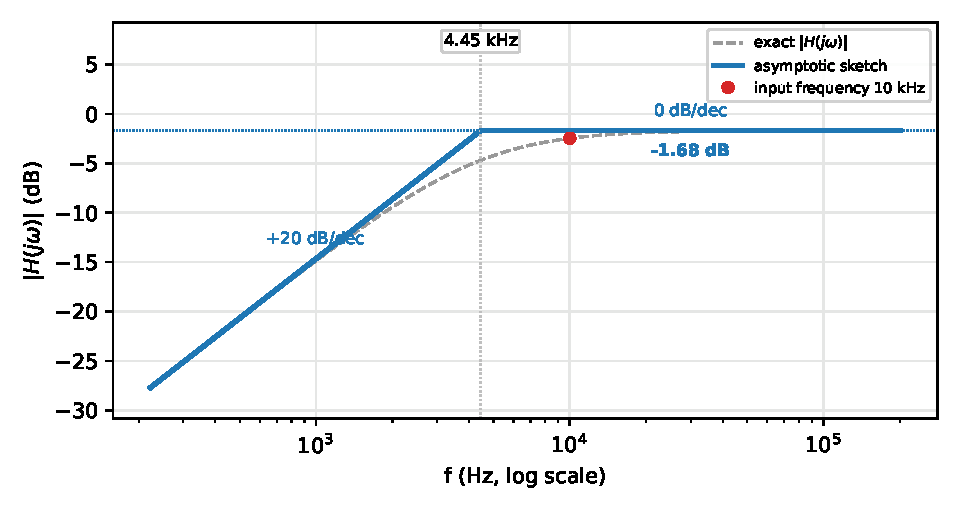
\includegraphics[width=0.78\linewidth,height=6.5cm,keepaspectratio]{p02_bode}\end{center}

{\small Blue: the straight-line sketch you are expected to draw. Dashed grey: the exact curve (about 3\,dB below the corner of an isolated pole). Red dot: the input frequency of Step 7.}
\solstep{7}{Total output (DC + AC)}The input is $V_i(t) = 0.002\sin\left(2\pi\cdot 10000\,t\right)$, so $\omega_{in} = 2\pi\cdot 10000 = 62800$\,rad/s. Put $s=j\omega_{in}$ in each factor (tool T5): magnitudes multiply, angles add.
{\small Rules: $\left|\frac{s}{s+p}\right| = \frac{\omega}{\sqrt{\omega^2+p^2}}$, $\angle = \frac{\pi}{2}-\tan^{-1}\frac{\omega}{p}$;\quad $\left|\frac{1}{1+s/p}\right| = \frac{1}{\sqrt{1+(\omega/p)^2}}$, $\angle = -\tan^{-1}\frac{\omega}{p}$;\quad $\left|1+\frac{s}{z}\right| = \sqrt{1+(\omega/z)^2}$, $\angle = \tan^{-1}\frac{\omega}{z}$;\quad a negative $K$ adds $-\pi$.}
\begin{center}\renewcommand{\arraystretch}{1.35}
\begin{tabular}{ccc}
\toprule
factor & magnitude & angle (rad) \\
\midrule
$0.825$ & $0.8246$ & $0$ \\
$\rule[-1.1em]{0pt}{2.8em}\dfrac{s}{s+2\pi\cdot 4.45\mathrm{k}}$ & $0.9136$ & $0.419$ \\
\textbf{total} & $\mathbf{0.7533}$ (product) & $\mathbf{0.419}$ (sum) \\
\bottomrule
\end{tabular}\end{center}

\begin{align*}
|H(j\omega_{in})| &= 0.753, \qquad \angle H(j\omega_{in}) = 0.419\ \mathrm{rad} \\
v_{o,ac}(t) &= 0.753\times 0.002\,\sin\left(2\pi\cdot 10000\,t + 0.419\right) = 0.00151\,\sin\left(2\pi\cdot 10000\,t + 0.419\right)
\end{align*}

Add the DC part from Step 2 (superposition):
\[
\boxed{V_o(t) = -4.3 + 0.00151\,\sin\left(2\pi\cdot 10000\,t + 0.419\right)\ \mathrm{V}}
\]
 Check the small-signal assumption: the AC voltage across the diode has amplitude about $1.51\,\mathrm{m}\mathrm{V}$, well below $nV_T = 45\,\mathrm{m}\mathrm{V}$ \checkmark.
\begin{ansbox}
$H(s) = 0.825\,\dfrac{s}{s+2\pi\cdot 4.45\mathrm{k}}$\quad (corners: 4.45 kHz)\\[4pt]
$V_o(t) = -4.3 + 0.00151\,\sin\left(2\pi\cdot 10000\,t + 0.419\right)\ \mathrm{V}$
\end{ansbox}

\newpage
\subsection*{Solution 3D.3 \hfill Easy}
\begin{center}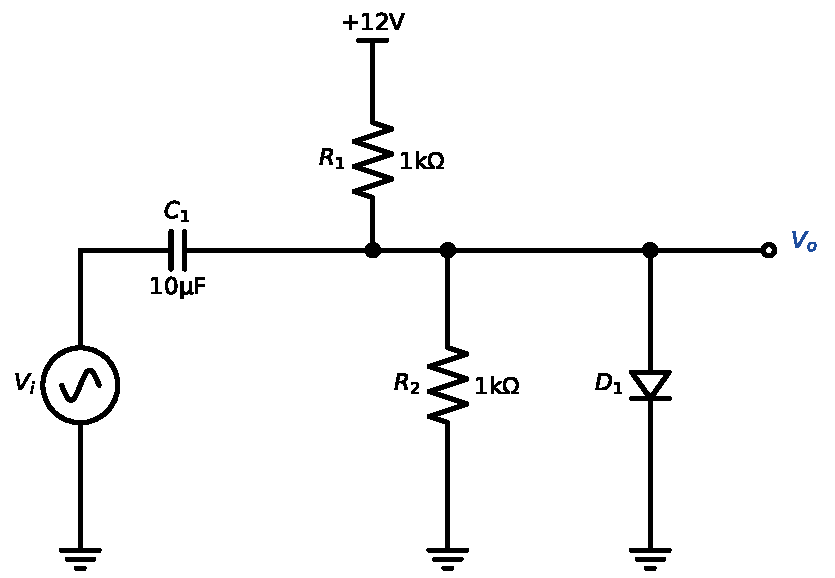
\includegraphics[width=0.9\linewidth,height=5cm,keepaspectratio]{p03_circuit}\end{center}
\solstep{1}{DC operating point}DC rules (tool T3): $v_i = 0$ and every capacitor is open ($C_{1}$). Assume the diode is ON (constant-voltage-drop model, $0.7$\,V) and solve the DC circuit:

Replace $D_{1}$ ON: a $0.7$\,V source ($V_{o} - 0 = 0.7$) carrying an unknown current $I_{D_{1}}$ from anode to cathode.

Equations (KCL at every node that is not an op-amp output, plus the diode voltages):\begin{align*}
&\text{KCL at }V_{o}: && \frac{V_{o} - 12}{R_{1}} + \frac{V_{o}}{R_{2}} + I_{D_{1}} = 0 \\
&\text{D1 ON}: && V_{o} - 0 = 0.7
\end{align*}


Solving these linear equations (substitute one into the other, as in Lecture 2) gives, with $V_i$ kept as a symbol:\begin{align*}
V_{o} &= 0.7 \\
I_{D_{1}} &= 10.6\ \mathrm{mA}
\end{align*}


 $I_{D_{1}} = 10.6\,\mathrm{m}\mathrm{A} > 0$ \checkmark, so the assumption holds.\[
\boxed{V_{o,dc} = 700\,\mathrm{m}\mathrm{V}}
\]

\solstep{2}{Small-signal resistance}$r_{d} = \frac{nV_T}{I_D} = \frac{1.8\times 25\,\mathrm{mV}}{10.6\,\mathrm{m}\mathrm{A}} = 4.25\,\Omega$ (tool T3). For the AC analysis the diode is just this resistor.
\solstep{3}{AC circuit}Set every DC supply to zero: each supply rail becomes AC ground. Replace every capacitor by $\frac{1}{sC}$ and every inductor by $sL$.
\begin{itemize}[leftmargin=*,itemsep=2pt]
\item $R_{1}$, $R_{2}$ both go from the same node to (AC) ground, so they are in parallel: $R_{12} = R_{1} \parallel R_{2} = 1\,\mathrm{k} \parallel 1\,\mathrm{k} = 500\,\Omega$.
\end{itemize}

AC equivalent circuit (nodes named for the next step):
\begin{center}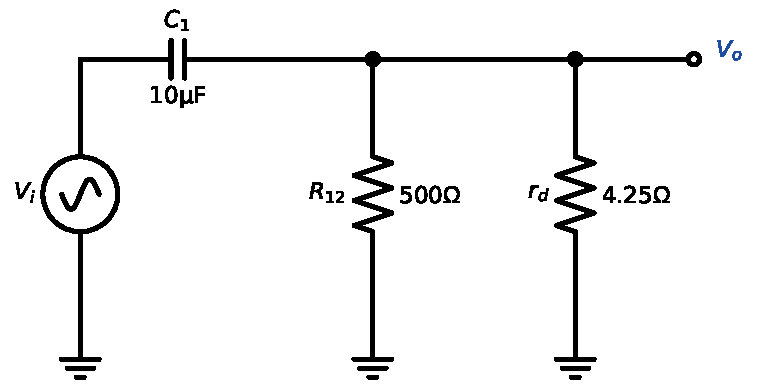
\includegraphics[width=0.95\linewidth,height=5.2cm,keepaspectratio]{p03_ac}\end{center}

\solstep{4}{Transfer function by a chain of dividers}Walk from the input to the output through the named nodes: $V_{i} \to V_{o}$. There is a single link, so $H(s)$ is just one voltage divider (tool T2).
Impedances seen \emph{looking right} from a node (everything from that node to ground, excluding what is on its left). Compute them from the far right toward the input:
\begin{align*}
Z_{o} &= R_{12} \parallel r_d = 4.21
\end{align*}

Now each link. {\small (Algebra tip: to simplify a fraction that contains fractions, multiply its top and bottom by every inner denominator; then divide top and bottom by the leading coefficient of the denominator so that it starts with a plain $s^n$.)}
\begin{align*}
\frac{V_{o}}{V_{i}} &= \frac{Z_{o}}{\frac{1}{sC_{1}} + Z_{o}} = \dfrac{s}{s + 23800}
\end{align*}
So:\[
H(s) = \dfrac{s}{s + 23800}
\]

\solstep{5}{Standard (Bode-ready) form}Find the roots. Every root $s=-p$ of the denominator is a \emph{pole}, every root $s=-z$ of the numerator is a \emph{zero}; $|p|$ and $|z|$ are the corner frequencies (rad/s).
\begin{itemize}[leftmargin=*,itemsep=2pt]
\item Numerator: it has the factor $s$ $\Rightarrow$ 1 zero at $s=0$.
\item Denominator: $s + 23800$; $s + 23800 = 0 \Rightarrow s = -23800$.
\end{itemize}

Factored form (leading coefficient in front):
\[
H(s) = 1\,\dfrac{s}{(s+23800)}
\]

Bode-ready form: rewrite every $(s+p) = p\left(1+\frac{s}{p}\right)$ and $(s+z) = z\left(1+\frac{s}{z}\right)$, and collect all constants into $K$. Each $s$ in the numerator is paired with one of the \emph{lowest} poles as $\frac{s}{s+p}$ (that factor is $\approx 1$ above $p$). Then every factor except $K$ is $\approx 1$ inside the pass-band:
\[
H(s) = 1\,\dfrac{s}{s+2\pi\cdot 3.78\mathrm{k}},\qquad K = 1
\]

\begin{center}\renewcommand{\arraystretch}{1.35}
\begin{tabular}{cccc}
\toprule
type & $\omega_c$ (rad/s) & $f_c=\omega_c/2\pi$ & slope change \\
\midrule
pole & $23800$ & 3.78 kHz & $-20$ dB/dec \\
\bottomrule
\end{tabular}\end{center}

\solstep{6}{Magnitude Bode plot}Below every corner $|H(s)|\approx 4.21\times 10^{-5}\,s$, so the plot starts with a slope of $+20$\,dB/dec. Then, moving right, each pole bends the line down by 20\,dB/dec and each zero bends it up by 20\,dB/dec (tool T6):
\begin{center}\renewcommand{\arraystretch}{1.35}
\begin{tabular}{lcl}
\toprule
frequency range & slope & asymptote level \\
\midrule
$f<$ 3.78 kHz & $+20$ dB/dec & 0 dB at end \\
$f>$ 3.78 kHz & $0$ dB/dec (flat) & 0 dB at start \\
\bottomrule
\end{tabular}\end{center}

The flat (pass-band) level is $20\log_{10}|K| = 20\log_{10}1 = 0$\,dB.
\begin{center}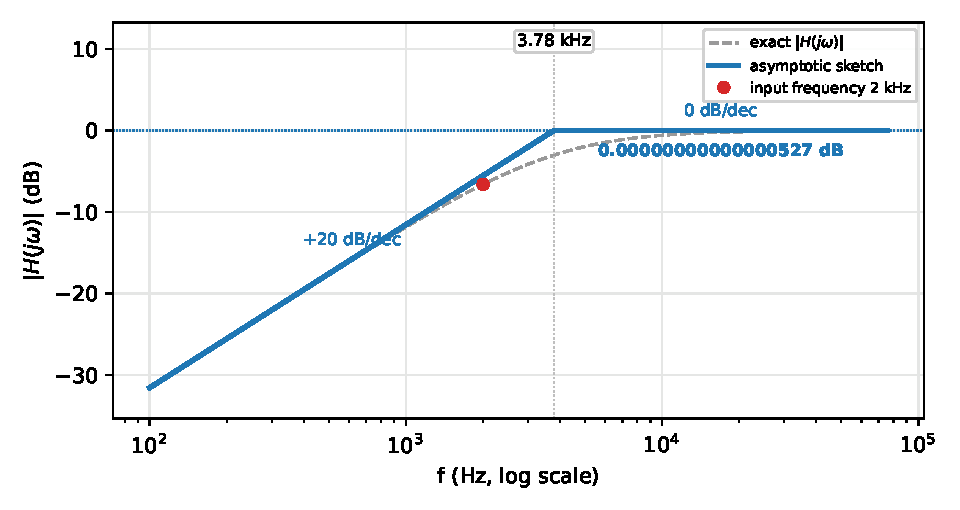
\includegraphics[width=0.78\linewidth,height=6.5cm,keepaspectratio]{p03_bode}\end{center}

{\small Blue: the straight-line sketch you are expected to draw. Dashed grey: the exact curve (about 3\,dB below the corner of an isolated pole). Red dot: the input frequency of Step 7.}
\solstep{7}{Total output (DC + AC)}The input is $V_i(t) = 0.001\sin\left(2\pi\cdot 2000\,t\right)$, so $\omega_{in} = 2\pi\cdot 2000 = 12600$\,rad/s. Put $s=j\omega_{in}$ in each factor (tool T5): magnitudes multiply, angles add.
{\small Rules: $\left|\frac{s}{s+p}\right| = \frac{\omega}{\sqrt{\omega^2+p^2}}$, $\angle = \frac{\pi}{2}-\tan^{-1}\frac{\omega}{p}$;\quad $\left|\frac{1}{1+s/p}\right| = \frac{1}{\sqrt{1+(\omega/p)^2}}$, $\angle = -\tan^{-1}\frac{\omega}{p}$;\quad $\left|1+\frac{s}{z}\right| = \sqrt{1+(\omega/z)^2}$, $\angle = \tan^{-1}\frac{\omega}{z}$;\quad a negative $K$ adds $-\pi$.}
\begin{center}\renewcommand{\arraystretch}{1.35}
\begin{tabular}{ccc}
\toprule
factor & magnitude & angle (rad) \\
\midrule
$1$ & $1$ & $0$ \\
$\rule[-1.1em]{0pt}{2.8em}\dfrac{s}{s+2\pi\cdot 3.78\mathrm{k}}$ & $0.4676$ & $1.08$ \\
\textbf{total} & $\mathbf{0.4676}$ (product) & $\mathbf{1.08}$ (sum) \\
\bottomrule
\end{tabular}\end{center}

\begin{align*}
|H(j\omega_{in})| &= 0.468, \qquad \angle H(j\omega_{in}) = 1.08\ \mathrm{rad} \\
v_{o,ac}(t) &= 0.468\times 0.001\,\sin\left(2\pi\cdot 2000\,t + 1.08\right) = 4.68\times 10^{-4}\,\sin\left(2\pi\cdot 2000\,t + 1.08\right)
\end{align*}

Add the DC part from Step 2 (superposition):
\[
\boxed{V_o(t) = 0.7 + 4.68\times 10^{-4}\,\sin\left(2\pi\cdot 2000\,t + 1.08\right)\ \mathrm{V}}
\]
 Check the small-signal assumption: the AC voltage across the diode has amplitude about $468\,\mu \mathrm{V}$, well below $nV_T = 45\,\mathrm{m}\mathrm{V}$ \checkmark.
\begin{ansbox}
$H(s) = 1\,\dfrac{s}{s+2\pi\cdot 3.78\mathrm{k}}$\quad (corners: 3.78 kHz)\\[4pt]
$V_o(t) = 0.7 + 4.68\times 10^{-4}\,\sin\left(2\pi\cdot 2000\,t + 1.08\right)\ \mathrm{V}$
\end{ansbox}

\newpage
\subsection*{Solution 3D.4 \hfill Easy}
\begin{center}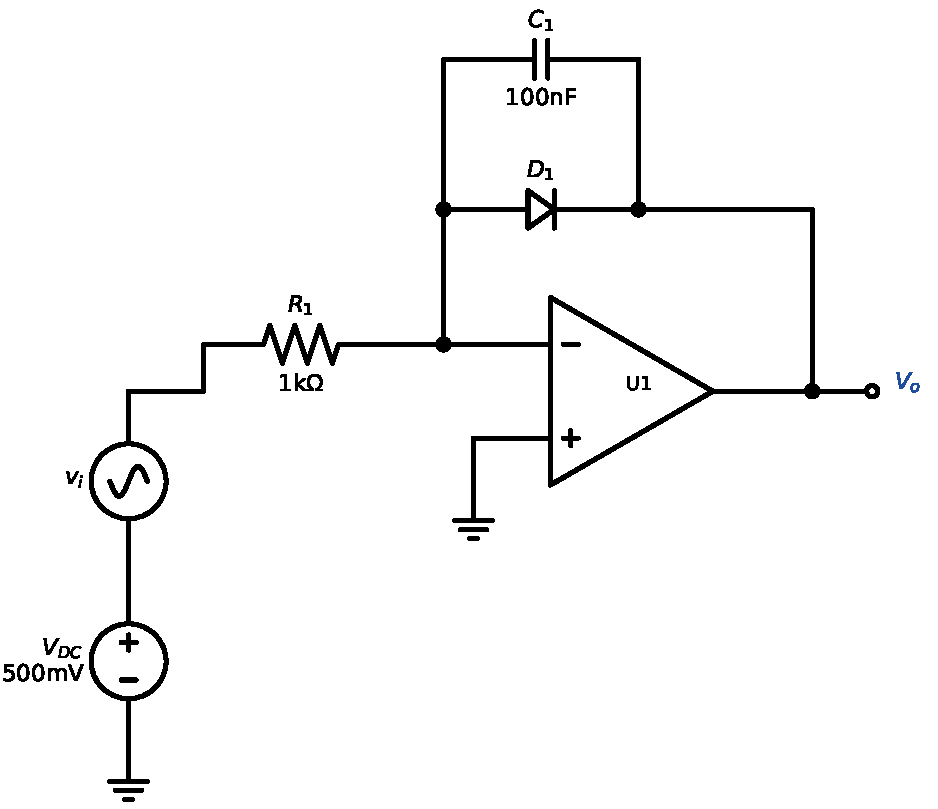
\includegraphics[width=0.9\linewidth,height=5cm,keepaspectratio]{p04_circuit}\end{center}
\solstep{1}{DC operating point}DC rules (tool T3): $v_i = 0$, so the input is just $V_{DC} = 500\,\mathrm{m}\mathrm{V}$; capacitors are open. The op-amp has negative feedback, so $V_- = V_+ = 0$ (virtual ground) and no current enters its inputs. The input current $\frac{V_{DC} - 0}{R_{1}} = 500\,\mu \mathrm{A}$ cannot enter the op-amp: all of it flows through the diode, $I_D = 500\,\mu \mathrm{A}$. Constant-voltage-drop model: $V_D = 0.7$\,V. The diode current flows from the $-$ input (at 0\,V) toward the output, so the output sits $V_D$ below it:\[
V_{o,dc} = -(V_D) = -700\,\mathrm{m}\mathrm{V}
\]
\[
\boxed{V_{o,dc} = -700\,\mathrm{m}\mathrm{V}}
\]

\solstep{2}{Small-signal resistance}$r_d = \frac{nV_T}{I_D} = \frac{1.8\times 25\,\mathrm{mV}}{500\,\mu \mathrm{A}} = 90\,\Omega$ (tool T3). For the AC analysis the diode is just this resistor, and $V_{DC}$ is replaced by a short (AC ground).
\solstep{3}{AC circuit}\begin{center}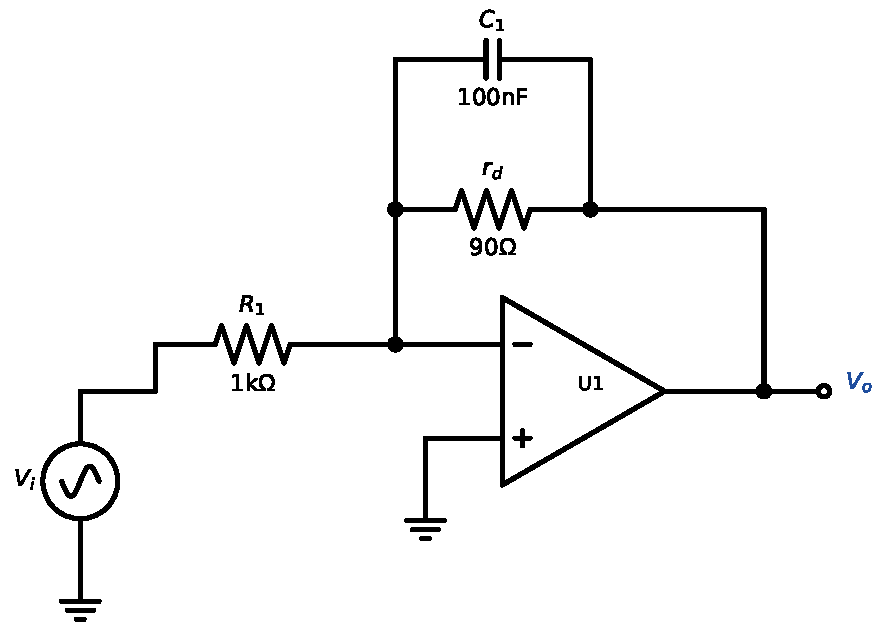
\includegraphics[width=0.9\linewidth,height=5cm,keepaspectratio]{p04_ac}\end{center}

\solstep{4}{Transfer function}\textbf{Block 1 (U1).} Inverting block: the $+$ input is grounded, so $V_- = V_+ = 0$ (virtual ground). The current $\frac{V_{i} - 0}{R_{1}}$ through $R_{1}$ cannot enter the op-amp, so all of it flows through $Z_{f1}$: $V_{o} = 0 - Z_{f1}\cdot\frac{V_{i}}{R_{1}}$.\begin{align*}
Z_{f1} &= r_d \parallel \frac{1}{sC_{1}} = \dfrac{10^{7}}{s + 1.11\times 10^{5}}
\end{align*}
\[
\frac{V_{o}}{V_{i}} = -\frac{Z_{f1}}{R_{1}} = \dfrac{-10000}{s + 1.11\times 10^{5}}
\]
So:\[
H(s) = \dfrac{-10000}{s + 1.11\times 10^{5}}
\]

\solstep{5}{Standard (Bode-ready) form}Find the roots. Every root $s=-p$ of the denominator is a \emph{pole}, every root $s=-z$ of the numerator is a \emph{zero}; $|p|$ and $|z|$ are the corner frequencies (rad/s).
\begin{itemize}[leftmargin=*,itemsep=2pt]
\item Denominator: $s + 1.11\times 10^{5}$; $s + 1.11\times 10^{5} = 0 \Rightarrow s = -1.11\times 10^{5}$.
\end{itemize}

Factored form (leading coefficient in front):
\[
H(s) = -10000\,\dfrac{1}{(s+1.11\times 10^{5})}
\]

Bode-ready form: rewrite every $(s+p) = p\left(1+\frac{s}{p}\right)$ and $(s+z) = z\left(1+\frac{s}{z}\right)$, and collect all constants into $K$. Then every factor except $K$ is $\approx 1$ inside the pass-band:
\[
H(s) = -0.09\,\dfrac{1}{1+\dfrac{s}{2\pi\cdot 17.7\mathrm{k}}},\qquad K = -0.09
\]

\begin{center}\renewcommand{\arraystretch}{1.35}
\begin{tabular}{cccc}
\toprule
type & $\omega_c$ (rad/s) & $f_c=\omega_c/2\pi$ & slope change \\
\midrule
pole & $1.11\times 10^{5}$ & 17.7 kHz & $-20$ dB/dec \\
\bottomrule
\end{tabular}\end{center}

\solstep{6}{Magnitude Bode plot}Below every corner, all factors are $\approx$ constant: $|H| \approx 0.09$ $= -20.9$\,dB (flat, 0 dB/dec). Then, moving right, each pole bends the line down by 20\,dB/dec and each zero bends it up by 20\,dB/dec (tool T6):
\begin{center}\renewcommand{\arraystretch}{1.35}
\begin{tabular}{lcl}
\toprule
frequency range & slope & asymptote level \\
\midrule
$f<$ 17.7 kHz & $0$ dB/dec (flat) & -20.9 dB at end \\
$f>$ 17.7 kHz & $-20$ dB/dec & -20.9 dB at start \\
\bottomrule
\end{tabular}\end{center}

The flat (pass-band) level is $20\log_{10}|K| = 20\log_{10}0.09 = -20.9$\,dB.
\begin{center}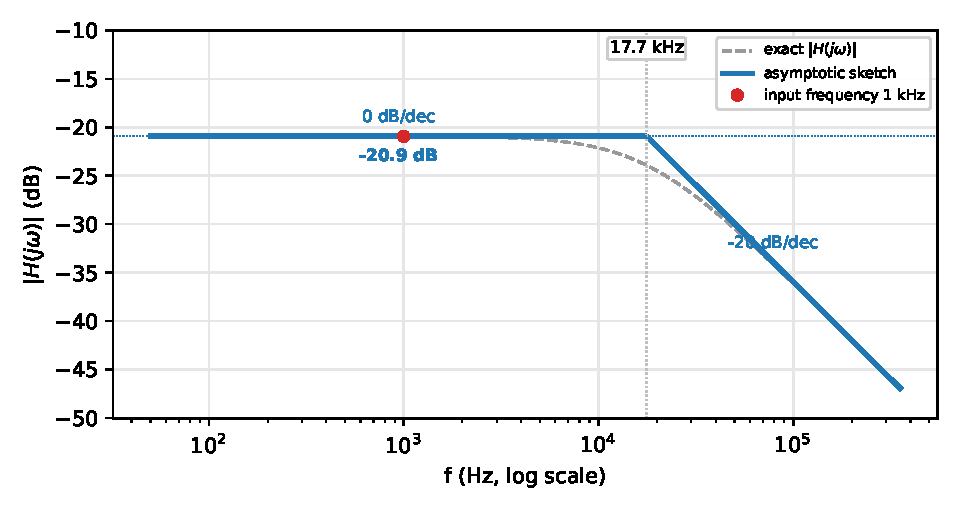
\includegraphics[width=0.78\linewidth,height=6.5cm,keepaspectratio]{p04_bode}\end{center}

{\small Blue: the straight-line sketch you are expected to draw. Dashed grey: the exact curve (about 3\,dB below the corner of an isolated pole). Red dot: the input frequency of Step 7.}
\solstep{7}{Total output (DC + AC)}The input is $V_i(t) = 0.02\sin\left(2\pi\cdot 1000\,t\right)$, so $\omega_{in} = 2\pi\cdot 1000 = 6280$\,rad/s. Put $s=j\omega_{in}$ in each factor (tool T5): magnitudes multiply, angles add.
{\small Rules: $\left|\frac{s}{s+p}\right| = \frac{\omega}{\sqrt{\omega^2+p^2}}$, $\angle = \frac{\pi}{2}-\tan^{-1}\frac{\omega}{p}$;\quad $\left|\frac{1}{1+s/p}\right| = \frac{1}{\sqrt{1+(\omega/p)^2}}$, $\angle = -\tan^{-1}\frac{\omega}{p}$;\quad $\left|1+\frac{s}{z}\right| = \sqrt{1+(\omega/z)^2}$, $\angle = \tan^{-1}\frac{\omega}{z}$;\quad a negative $K$ adds $-\pi$.}
\begin{center}\renewcommand{\arraystretch}{1.35}
\begin{tabular}{ccc}
\toprule
factor & magnitude & angle (rad) \\
\midrule
$-0.09$ & $0.09$ & $-3.14$ \\
$\rule[-1.7em]{0pt}{4em}\dfrac{1}{1+\dfrac{s}{2\pi\cdot 17.7\mathrm{k}}}$ & $0.9984$ & $-0.0565$ \\
\textbf{total} & $\mathbf{0.08986}$ (product) & $\mathbf{-3.2}$ (sum) \\
\bottomrule
\end{tabular}\end{center}

\begin{align*}
|H(j\omega_{in})| &= 0.0899, \qquad \angle H(j\omega_{in}) = -3.2\ \mathrm{rad} \\
v_{o,ac}(t) &= 0.0899\times 0.02\,\sin\left(2\pi\cdot 1000\,t - 3.2\right) = 0.0018\,\sin\left(2\pi\cdot 1000\,t - 3.2\right)
\end{align*}

Add the DC part from Step 2 (superposition):
\[
\boxed{V_o(t) = -0.7 + 0.0018\,\sin\left(2\pi\cdot 1000\,t - 3.2\right)\ \mathrm{V}}
\]
 Check the small-signal assumption: the AC voltage across the diode has amplitude about $1.8\,\mathrm{m}\mathrm{V}$, well below $nV_T = 45\,\mathrm{m}\mathrm{V}$ \checkmark.
\begin{ansbox}
$H(s) = -0.09\,\dfrac{1}{1+\dfrac{s}{2\pi\cdot 17.7\mathrm{k}}}$\quad (corners: 17.7 kHz)\\[4pt]
$V_o(t) = -0.7 + 0.0018\,\sin\left(2\pi\cdot 1000\,t - 3.2\right)\ \mathrm{V}$
\end{ansbox}

\newpage
\subsection*{Solution 3D.5 \hfill Easy}
\begin{center}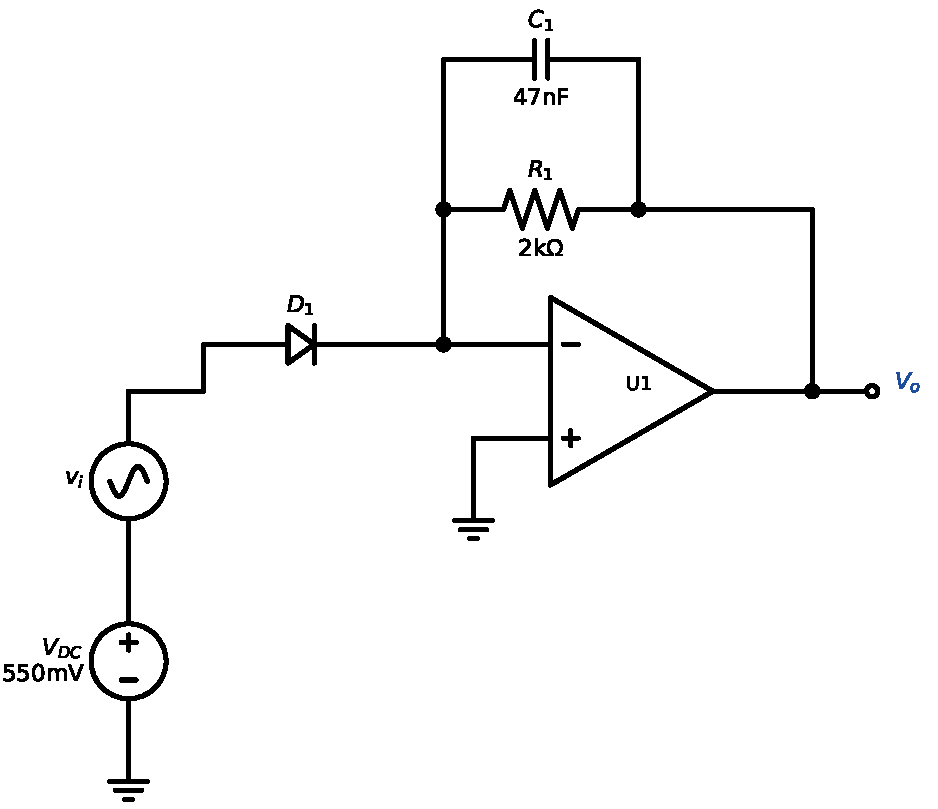
\includegraphics[width=0.9\linewidth,height=5cm,keepaspectratio]{p05_circuit}\end{center}
\solstep{1}{DC operating point}DC rules (tool T3): $v_i = 0$, so the input is just $V_{DC} = 550\,\mathrm{m}\mathrm{V}$; capacitors are open. The op-amp has negative feedback, so $V_- = V_+ = 0$ (virtual ground) and no current enters its inputs. The diode sits between $V_{DC}$ and the virtual ground, so $V_D = V_{DC} = 550\,\mathrm{m}\mathrm{V}$ and the exponential model (tool T1) gives\[
I_D = I_S\,e^{V_D/nV_T} = 2.6\,\mathrm{n}\mathrm{A}\times \exp\left(\frac{0.55}{1.8\times 0.025}\right) = 528\,\mu \mathrm{A}
\]
 All of $I_D$ continues through the feedback resistor $R_{1}$ (the capacitor is open), so\[
V_{o,dc} = 0 - R_{1}I_D = -2000\times5.285\times 10^{-4} = -1.06\,\mathrm{V}
\]
\[
\boxed{V_{o,dc} = -1.06\,\mathrm{V}}
\]

\solstep{2}{Small-signal resistance}$r_d = \frac{nV_T}{I_D} = \frac{1.8\times 25\,\mathrm{mV}}{528\,\mu \mathrm{A}} = 85.2\,\Omega$ (tool T3). For the AC analysis the diode is just this resistor, and $V_{DC}$ is replaced by a short (AC ground).
\solstep{3}{AC circuit}\begin{center}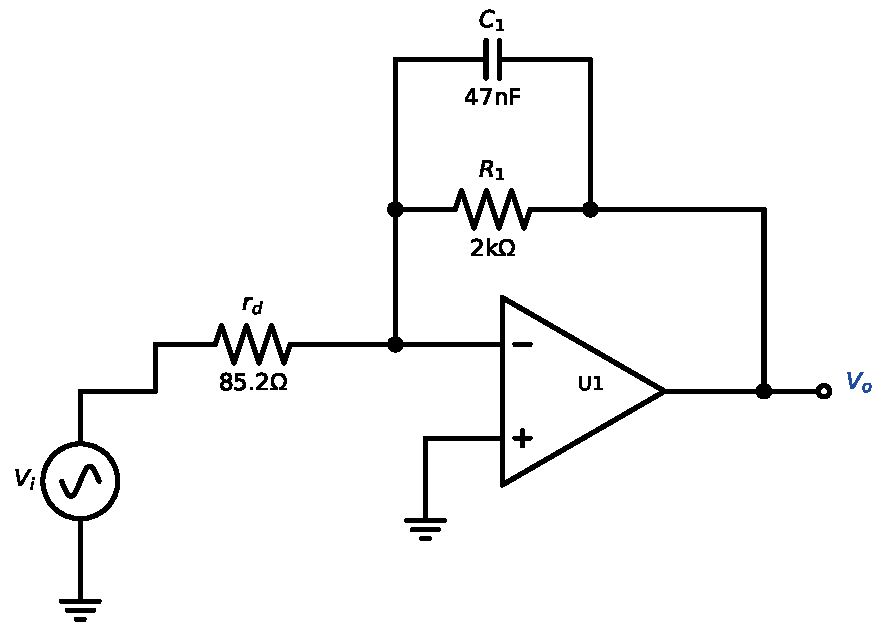
\includegraphics[width=0.9\linewidth,height=5cm,keepaspectratio]{p05_ac}\end{center}

\solstep{4}{Transfer function}\textbf{Block 1 (U1).} Inverting block: the $+$ input is grounded, so $V_- = V_+ = 0$ (virtual ground). The current $\frac{V_{i} - 0}{r_d}$ through $r_d$ cannot enter the op-amp, so all of it flows through $Z_{f1}$: $V_{o} = 0 - Z_{f1}\cdot\frac{V_{i}}{r_d}$.\begin{align*}
Z_{f1} &= R_{1} \parallel \frac{1}{sC_{1}} = \dfrac{2.13\times 10^{7}}{s + 10600}
\end{align*}
\[
\frac{V_{o}}{V_{i}} = -\frac{Z_{f1}}{r_d} = \dfrac{-2.5\times 10^{5}}{s + 10600}
\]
So:\[
H(s) = \dfrac{-2.5\times 10^{5}}{s + 10600}
\]

\solstep{5}{Standard (Bode-ready) form}Find the roots. Every root $s=-p$ of the denominator is a \emph{pole}, every root $s=-z$ of the numerator is a \emph{zero}; $|p|$ and $|z|$ are the corner frequencies (rad/s).
\begin{itemize}[leftmargin=*,itemsep=2pt]
\item Denominator: $s + 10600$; $s + 10600 = 0 \Rightarrow s = -10600$.
\end{itemize}

Factored form (leading coefficient in front):
\[
H(s) = -2.5\times 10^{5}\,\dfrac{1}{(s+10600)}
\]

Bode-ready form: rewrite every $(s+p) = p\left(1+\frac{s}{p}\right)$ and $(s+z) = z\left(1+\frac{s}{z}\right)$, and collect all constants into $K$. Then every factor except $K$ is $\approx 1$ inside the pass-band:
\[
H(s) = -23.5\,\dfrac{1}{1+\dfrac{s}{2\pi\cdot 1.69\mathrm{k}}},\qquad K = -23.5
\]

\begin{center}\renewcommand{\arraystretch}{1.35}
\begin{tabular}{cccc}
\toprule
type & $\omega_c$ (rad/s) & $f_c=\omega_c/2\pi$ & slope change \\
\midrule
pole & $10600$ & 1.69 kHz & $-20$ dB/dec \\
\bottomrule
\end{tabular}\end{center}

\solstep{6}{Magnitude Bode plot}Below every corner, all factors are $\approx$ constant: $|H| \approx 23.5$ $= 27.4$\,dB (flat, 0 dB/dec). Then, moving right, each pole bends the line down by 20\,dB/dec and each zero bends it up by 20\,dB/dec (tool T6):
\begin{center}\renewcommand{\arraystretch}{1.35}
\begin{tabular}{lcl}
\toprule
frequency range & slope & asymptote level \\
\midrule
$f<$ 1.69 kHz & $0$ dB/dec (flat) & 27.4 dB at end \\
$f>$ 1.69 kHz & $-20$ dB/dec & 27.4 dB at start \\
\bottomrule
\end{tabular}\end{center}

The flat (pass-band) level is $20\log_{10}|K| = 20\log_{10}23.5 = 27.4$\,dB.
\begin{center}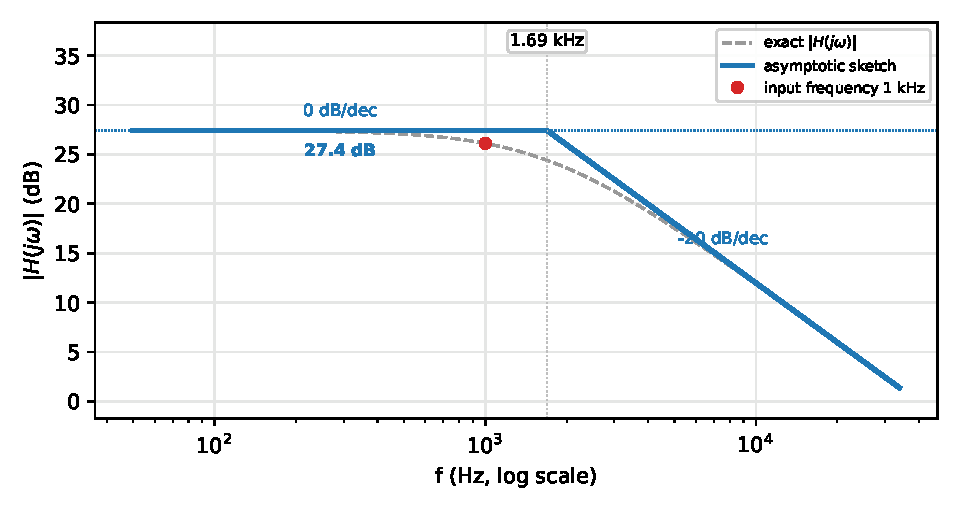
\includegraphics[width=0.78\linewidth,height=6.5cm,keepaspectratio]{p05_bode}\end{center}

{\small Blue: the straight-line sketch you are expected to draw. Dashed grey: the exact curve (about 3\,dB below the corner of an isolated pole). Red dot: the input frequency of Step 7.}
\solstep{7}{Total output (DC + AC)}The input is $V_i(t) = 0.002\sin\left(2\pi\cdot 1000\,t\right)$, so $\omega_{in} = 2\pi\cdot 1000 = 6280$\,rad/s. Put $s=j\omega_{in}$ in each factor (tool T5): magnitudes multiply, angles add.
{\small Rules: $\left|\frac{s}{s+p}\right| = \frac{\omega}{\sqrt{\omega^2+p^2}}$, $\angle = \frac{\pi}{2}-\tan^{-1}\frac{\omega}{p}$;\quad $\left|\frac{1}{1+s/p}\right| = \frac{1}{\sqrt{1+(\omega/p)^2}}$, $\angle = -\tan^{-1}\frac{\omega}{p}$;\quad $\left|1+\frac{s}{z}\right| = \sqrt{1+(\omega/z)^2}$, $\angle = \tan^{-1}\frac{\omega}{z}$;\quad a negative $K$ adds $-\pi$.}
\begin{center}\renewcommand{\arraystretch}{1.35}
\begin{tabular}{ccc}
\toprule
factor & magnitude & angle (rad) \\
\midrule
$-23.5$ & $23.49$ & $-3.14$ \\
$\rule[-1.7em]{0pt}{4em}\dfrac{1}{1+\dfrac{s}{2\pi\cdot 1.69\mathrm{k}}}$ & $0.861$ & $-0.533$ \\
\textbf{total} & $\mathbf{20.22}$ (product) & $\mathbf{-3.68}$ (sum) \\
\bottomrule
\end{tabular}\end{center}

\begin{align*}
|H(j\omega_{in})| &= 20.2, \qquad \angle H(j\omega_{in}) = -3.68\ \mathrm{rad} \\
v_{o,ac}(t) &= 20.2\times 0.002\,\sin\left(2\pi\cdot 1000\,t - 3.68\right) = 0.0404\,\sin\left(2\pi\cdot 1000\,t - 3.68\right)
\end{align*}

Add the DC part from Step 2 (superposition):
\[
\boxed{V_o(t) = -1.06 + 0.0404\,\sin\left(2\pi\cdot 1000\,t - 3.68\right)\ \mathrm{V}}
\]
 Check the small-signal assumption: the AC voltage across the diode has amplitude about $2\,\mathrm{m}\mathrm{V}$, well below $nV_T = 45\,\mathrm{m}\mathrm{V}$ \checkmark.
\begin{ansbox}
$H(s) = -23.5\,\dfrac{1}{1+\dfrac{s}{2\pi\cdot 1.69\mathrm{k}}}$\quad (corners: 1.69 kHz)\\[4pt]
$V_o(t) = -1.06 + 0.0404\,\sin\left(2\pi\cdot 1000\,t - 3.68\right)\ \mathrm{V}$
\end{ansbox}

\newpage
\subsection*{Solution 3D.6 \hfill Easy}
\begin{center}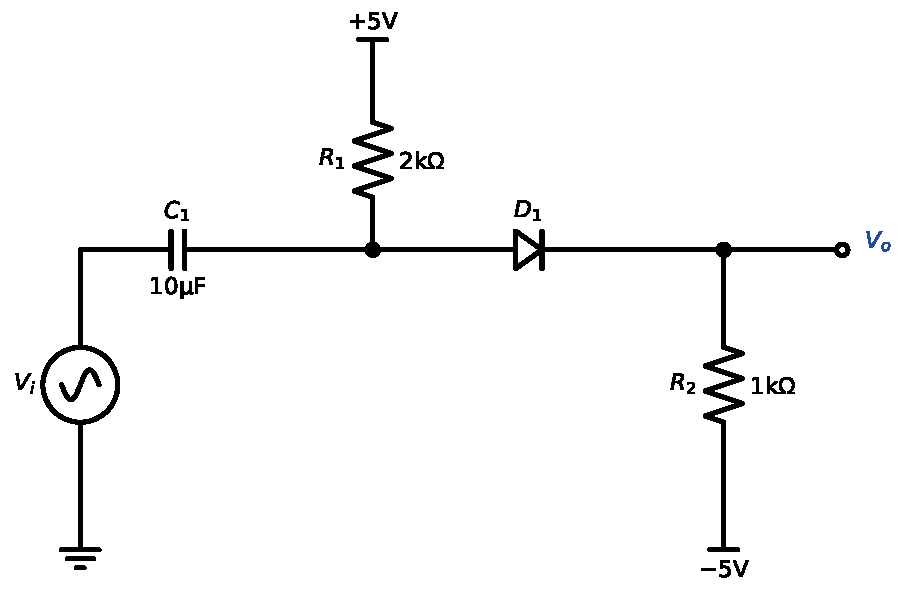
\includegraphics[width=0.9\linewidth,height=5cm,keepaspectratio]{p06_circuit}\end{center}
\solstep{1}{DC operating point}DC rules (tool T3): $v_i = 0$ and every capacitor is open ($C_{1}$). Assume the diode is ON (constant-voltage-drop model, $0.7$\,V) and solve the DC circuit:

Replace $D_{1}$ ON: a $0.7$\,V source ($V_{1} - V_{o} = 0.7$) carrying an unknown current $I_{D_{1}}$ from anode to cathode.

Equations (KCL at every node that is not an op-amp output, plus the diode voltages):\begin{align*}
&\text{KCL at }V_{1}: && \frac{V_{1} - 5}{R_{1}} + I_{D_{1}} = 0 \\
&\text{KCL at }V_{o}: && \frac{V_{o} - -5}{R_{2}} - I_{D_{1}} = 0 \\
&\text{D1 ON}: && V_{1} - V_{o} = 0.7
\end{align*}


Solving these linear equations (substitute one into the other, as in Lecture 2) gives, with $V_i$ kept as a symbol:\begin{align*}
V_{o} &= -1.9 \\
I_{D_{1}} &= 3.1\ \mathrm{mA}
\end{align*}


 $I_{D_{1}} = 3.1\,\mathrm{m}\mathrm{A} > 0$ \checkmark, so the assumption holds.\[
\boxed{V_{o,dc} = -1.9\,\mathrm{V}}
\]

\solstep{2}{Small-signal resistance}$r_{d} = \frac{nV_T}{I_D} = \frac{1.8\times 25\,\mathrm{mV}}{3.1\,\mathrm{m}\mathrm{A}} = 14.5\,\Omega$ (tool T3). For the AC analysis the diode is just this resistor.
\solstep{3}{AC circuit}Set every DC supply to zero: each supply rail becomes AC ground. Replace every capacitor by $\frac{1}{sC}$ and every inductor by $sL$.
AC equivalent circuit (nodes named for the next step):
\begin{center}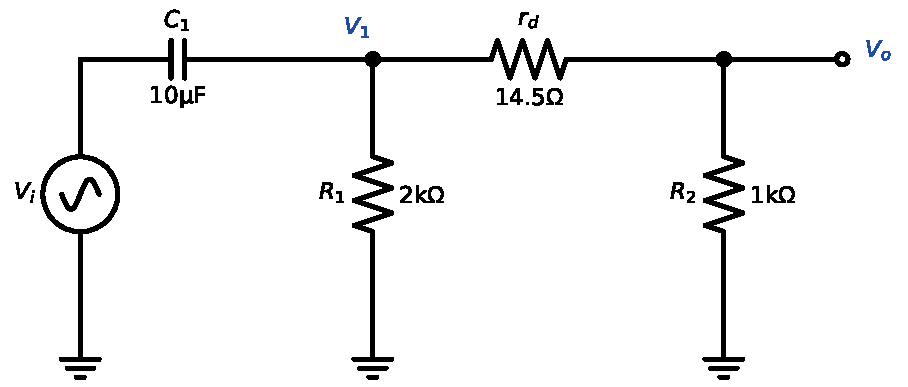
\includegraphics[width=0.95\linewidth,height=5.2cm,keepaspectratio]{p06_ac}\end{center}

\solstep{4}{Transfer function by a chain of dividers}Walk from the input to the output through the named nodes: $V_{i} \to V_{1} \to V_{o}$. The transfer function is the product of the node-to-node ratios (each one is a simple divider, tool T2, or a dependent source, tool T4):
\[
H(s) = \frac{V_o}{V_i} = \frac{V_{1}}{V_{i}}\cdot\frac{V_{o}}{V_{1}}
\]

Impedances seen \emph{looking right} from a node (everything from that node to ground, excluding what is on its left). Compute them from the far right toward the input:
\begin{align*}
Z_{1} &= R_{1} \parallel \left(r_d + R_{2}\right) = 673
\end{align*}

Now each link. {\small (Algebra tip: to simplify a fraction that contains fractions, multiply its top and bottom by every inner denominator; then divide top and bottom by the leading coefficient of the denominator so that it starts with a plain $s^n$.)}
\begin{align*}
\frac{V_{1}}{V_{i}} &= \frac{Z_{1}}{\frac{1}{sC_{1}} + Z_{1}} = \dfrac{s}{s + 149} \\
\frac{V_{o}}{V_{1}} &= \frac{R_{2}}{r_d + R_{2}} = 0.986
\end{align*}
Multiply the links and simplify:\[
H(s) = \dfrac{0.986\,s}{s + 149}
\]

\solstep{5}{Standard (Bode-ready) form}Find the roots. Every root $s=-p$ of the denominator is a \emph{pole}, every root $s=-z$ of the numerator is a \emph{zero}; $|p|$ and $|z|$ are the corner frequencies (rad/s).
\begin{itemize}[leftmargin=*,itemsep=2pt]
\item Numerator: it has the factor $s$ $\Rightarrow$ 1 zero at $s=0$.
\item Denominator: $s + 149$; $s + 149 = 0 \Rightarrow s = -149$.
\end{itemize}

Factored form (leading coefficient in front):
\[
H(s) = 0.986\,\dfrac{s}{(s+149)}
\]

Bode-ready form: rewrite every $(s+p) = p\left(1+\frac{s}{p}\right)$ and $(s+z) = z\left(1+\frac{s}{z}\right)$, and collect all constants into $K$. Each $s$ in the numerator is paired with one of the \emph{lowest} poles as $\frac{s}{s+p}$ (that factor is $\approx 1$ above $p$). Then every factor except $K$ is $\approx 1$ inside the pass-band:
\[
H(s) = 0.986\,\dfrac{s}{s+2\pi\cdot 23.6},\qquad K = 0.986
\]

\begin{center}\renewcommand{\arraystretch}{1.35}
\begin{tabular}{cccc}
\toprule
type & $\omega_c$ (rad/s) & $f_c=\omega_c/2\pi$ & slope change \\
\midrule
pole & $149$ & 23.6 Hz & $-20$ dB/dec \\
\bottomrule
\end{tabular}\end{center}

\solstep{6}{Magnitude Bode plot}Below every corner $|H(s)|\approx 0.00663\,s$, so the plot starts with a slope of $+20$\,dB/dec. Then, moving right, each pole bends the line down by 20\,dB/dec and each zero bends it up by 20\,dB/dec (tool T6):
\begin{center}\renewcommand{\arraystretch}{1.35}
\begin{tabular}{lcl}
\toprule
frequency range & slope & asymptote level \\
\midrule
$f<$ 23.6 Hz & $+20$ dB/dec & -0.125 dB at end \\
$f>$ 23.6 Hz & $0$ dB/dec (flat) & -0.125 dB at start \\
\bottomrule
\end{tabular}\end{center}

The flat (pass-band) level is $20\log_{10}|K| = 20\log_{10}0.986 = -0.125$\,dB.
\begin{center}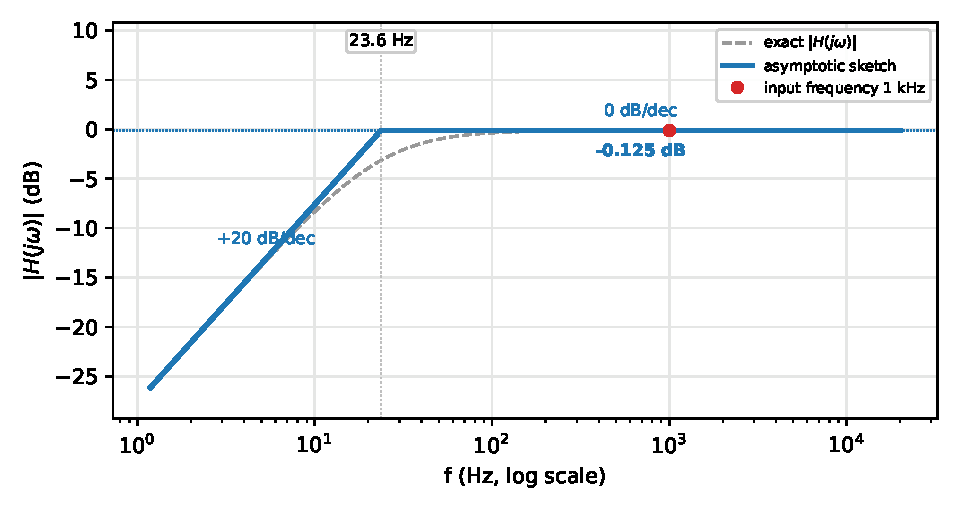
\includegraphics[width=0.78\linewidth,height=6.5cm,keepaspectratio]{p06_bode}\end{center}

{\small Blue: the straight-line sketch you are expected to draw. Dashed grey: the exact curve (about 3\,dB below the corner of an isolated pole). Red dot: the input frequency of Step 7.}
\solstep{7}{Total output (DC + AC)}The input is $V_i(t) = 0.005\sin\left(2\pi\cdot 1000\,t\right)$, so $\omega_{in} = 2\pi\cdot 1000 = 6280$\,rad/s. Put $s=j\omega_{in}$ in each factor (tool T5): magnitudes multiply, angles add.
{\small Rules: $\left|\frac{s}{s+p}\right| = \frac{\omega}{\sqrt{\omega^2+p^2}}$, $\angle = \frac{\pi}{2}-\tan^{-1}\frac{\omega}{p}$;\quad $\left|\frac{1}{1+s/p}\right| = \frac{1}{\sqrt{1+(\omega/p)^2}}$, $\angle = -\tan^{-1}\frac{\omega}{p}$;\quad $\left|1+\frac{s}{z}\right| = \sqrt{1+(\omega/z)^2}$, $\angle = \tan^{-1}\frac{\omega}{z}$;\quad a negative $K$ adds $-\pi$.}
\begin{center}\renewcommand{\arraystretch}{1.35}
\begin{tabular}{ccc}
\toprule
factor & magnitude & angle (rad) \\
\midrule
$0.986$ & $0.9857$ & $0$ \\
$\rule[-1.1em]{0pt}{2.8em}\dfrac{s}{s+2\pi\cdot 23.6}$ & $0.9997$ & $0.0236$ \\
\textbf{total} & $\mathbf{0.9854}$ (product) & $\mathbf{0.0236}$ (sum) \\
\bottomrule
\end{tabular}\end{center}

\begin{align*}
|H(j\omega_{in})| &= 0.985, \qquad \angle H(j\omega_{in}) = 0.0236\ \mathrm{rad} \\
v_{o,ac}(t) &= 0.985\times 0.005\,\sin\left(2\pi\cdot 1000\,t + 0.0236\right) = 0.00493\,\sin\left(2\pi\cdot 1000\,t + 0.0236\right)
\end{align*}

Add the DC part from Step 2 (superposition):
\[
\boxed{V_o(t) = -1.9 + 0.00493\,\sin\left(2\pi\cdot 1000\,t + 0.0236\right)\ \mathrm{V}}
\]
 Check the small-signal assumption: the AC voltage across the diode has amplitude about $71.5\,\mu \mathrm{V}$, well below $nV_T = 45\,\mathrm{m}\mathrm{V}$ \checkmark.
\begin{ansbox}
$H(s) = 0.986\,\dfrac{s}{s+2\pi\cdot 23.6}$\quad (corners: 23.6 Hz)\\[4pt]
$V_o(t) = -1.9 + 0.00493\,\sin\left(2\pi\cdot 1000\,t + 0.0236\right)\ \mathrm{V}$
\end{ansbox}

\newpage
\subsection*{Solution 3D.7 \hfill Medium}
\begin{center}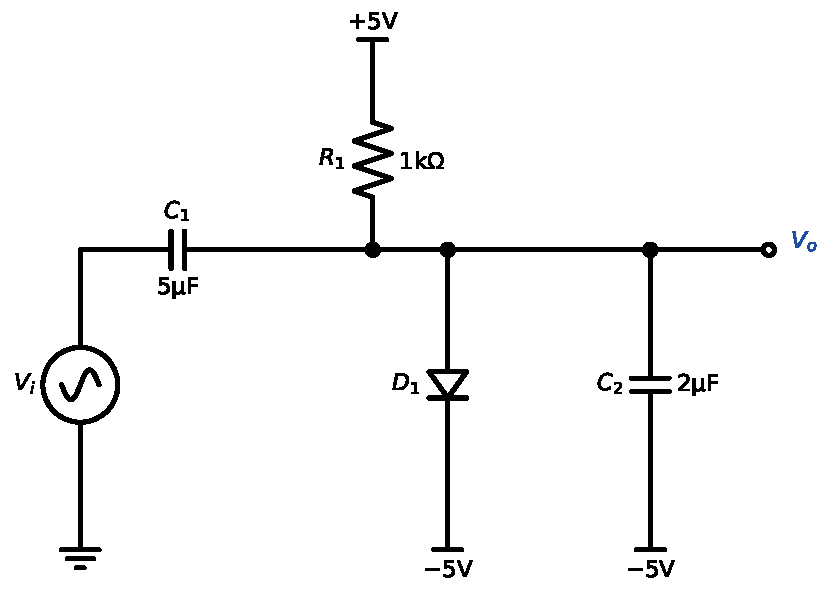
\includegraphics[width=0.9\linewidth,height=5cm,keepaspectratio]{p07_circuit}\end{center}
\solstep{1}{DC operating point}DC rules (tool T3): $v_i = 0$ and every capacitor is open ($C_{1}, C_{2}$). Assume the diode is ON (constant-voltage-drop model, $0.7$\,V) and solve the DC circuit:

Replace $D_{1}$ ON: a $0.7$\,V source ($V_{o} - -5 = 0.7$) carrying an unknown current $I_{D_{1}}$ from anode to cathode.

Equations (KCL at every node that is not an op-amp output, plus the diode voltages):\begin{align*}
&\text{KCL at }V_{o}: && \frac{V_{o} - 5}{R_{1}} + I_{D_{1}} = 0 \\
&\text{D1 ON}: && V_{o} - -5 = 0.7
\end{align*}


Solving these linear equations (substitute one into the other, as in Lecture 2) gives, with $V_i$ kept as a symbol:\begin{align*}
V_{o} &= -4.3 \\
I_{D_{1}} &= 9.3\ \mathrm{mA}
\end{align*}


 $I_{D_{1}} = 9.3\,\mathrm{m}\mathrm{A} > 0$ \checkmark, so the assumption holds.\[
\boxed{V_{o,dc} = -4.3\,\mathrm{V}}
\]

\solstep{2}{Small-signal resistance}$r_{d} = \frac{nV_T}{I_D} = \frac{1.8\times 25\,\mathrm{mV}}{9.3\,\mathrm{m}\mathrm{A}} = 4.84\,\Omega$ (tool T3). For the AC analysis the diode is just this resistor.
\solstep{3}{AC circuit}Set every DC supply to zero: each supply rail becomes AC ground. Replace every capacitor by $\frac{1}{sC}$ and every inductor by $sL$.
AC equivalent circuit (nodes named for the next step):
\begin{center}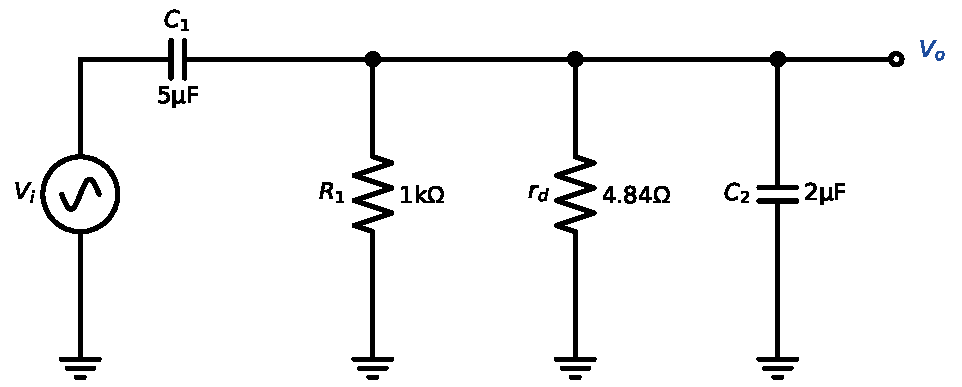
\includegraphics[width=0.95\linewidth,height=5.2cm,keepaspectratio]{p07_ac}\end{center}

\solstep{4}{Transfer function by a chain of dividers}Walk from the input to the output through the named nodes: $V_{i} \to V_{o}$. There is a single link, so $H(s)$ is just one voltage divider (tool T2).
Impedances seen \emph{looking right} from a node (everything from that node to ground, excluding what is on its left). Compute them from the far right toward the input:
\begin{align*}
Z_{o} &= R_{1} \parallel r_d \parallel \frac{1}{sC_{2}} = \dfrac{5\times 10^{5}}{s + 1.04\times 10^{5}}
\end{align*}

Now each link. {\small (Algebra tip: to simplify a fraction that contains fractions, multiply its top and bottom by every inner denominator; then divide top and bottom by the leading coefficient of the denominator so that it starts with a plain $s^n$.)}
\begin{align*}
\frac{V_{o}}{V_{i}} &= \frac{Z_{o}}{\frac{1}{sC_{1}} + Z_{o}} = \dfrac{0.714\,s}{s + 29700}
\end{align*}
So:\[
H(s) = \dfrac{0.714\,s}{s + 29700}
\]

\solstep{5}{Standard (Bode-ready) form}Find the roots. Every root $s=-p$ of the denominator is a \emph{pole}, every root $s=-z$ of the numerator is a \emph{zero}; $|p|$ and $|z|$ are the corner frequencies (rad/s).
\begin{itemize}[leftmargin=*,itemsep=2pt]
\item Numerator: it has the factor $s$ $\Rightarrow$ 1 zero at $s=0$.
\item Denominator: $s + 29700$; $s + 29700 = 0 \Rightarrow s = -29700$.
\end{itemize}

Factored form (leading coefficient in front):
\[
H(s) = 0.714\,\dfrac{s}{(s+29700)}
\]

Bode-ready form: rewrite every $(s+p) = p\left(1+\frac{s}{p}\right)$ and $(s+z) = z\left(1+\frac{s}{z}\right)$, and collect all constants into $K$. Each $s$ in the numerator is paired with one of the \emph{lowest} poles as $\frac{s}{s+p}$ (that factor is $\approx 1$ above $p$). Then every factor except $K$ is $\approx 1$ inside the pass-band:
\[
H(s) = 0.714\,\dfrac{s}{s+2\pi\cdot 4.72\mathrm{k}},\qquad K = 0.714
\]

\begin{center}\renewcommand{\arraystretch}{1.35}
\begin{tabular}{cccc}
\toprule
type & $\omega_c$ (rad/s) & $f_c=\omega_c/2\pi$ & slope change \\
\midrule
pole & $29700$ & 4.72 kHz & $-20$ dB/dec \\
\bottomrule
\end{tabular}\end{center}

\solstep{6}{Magnitude Bode plot}Below every corner $|H(s)|\approx 2.41\times 10^{-5}\,s$, so the plot starts with a slope of $+20$\,dB/dec. Then, moving right, each pole bends the line down by 20\,dB/dec and each zero bends it up by 20\,dB/dec (tool T6):
\begin{center}\renewcommand{\arraystretch}{1.35}
\begin{tabular}{lcl}
\toprule
frequency range & slope & asymptote level \\
\midrule
$f<$ 4.72 kHz & $+20$ dB/dec & -2.92 dB at end \\
$f>$ 4.72 kHz & $0$ dB/dec (flat) & -2.92 dB at start \\
\bottomrule
\end{tabular}\end{center}

The flat (pass-band) level is $20\log_{10}|K| = 20\log_{10}0.714 = -2.92$\,dB.
\begin{center}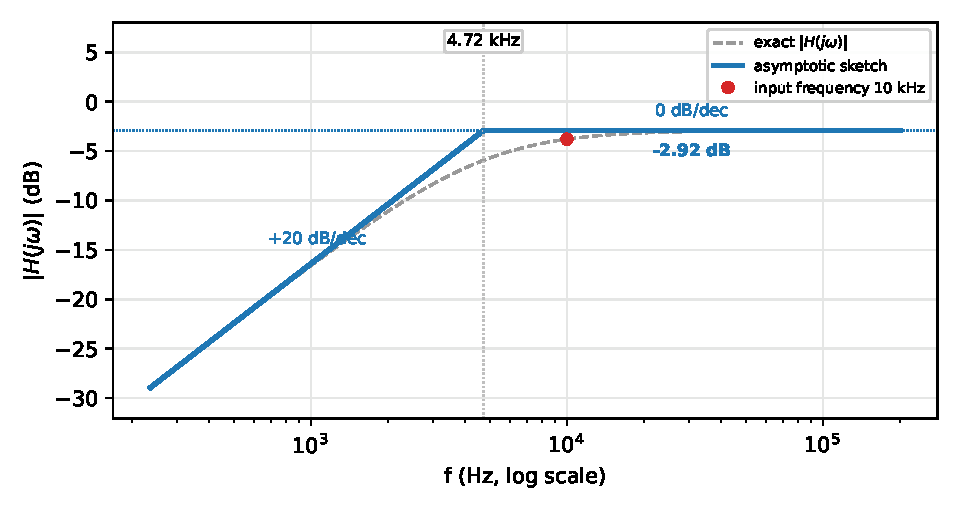
\includegraphics[width=0.78\linewidth,height=6.5cm,keepaspectratio]{p07_bode}\end{center}

{\small Blue: the straight-line sketch you are expected to draw. Dashed grey: the exact curve (about 3\,dB below the corner of an isolated pole). Red dot: the input frequency of Step 7.}
\solstep{7}{Total output (DC + AC)}The input is $V_i(t) = 0.002\sin\left(2\pi\cdot 10000\,t\right)$, so $\omega_{in} = 2\pi\cdot 10000 = 62800$\,rad/s. Put $s=j\omega_{in}$ in each factor (tool T5): magnitudes multiply, angles add.
{\small Rules: $\left|\frac{s}{s+p}\right| = \frac{\omega}{\sqrt{\omega^2+p^2}}$, $\angle = \frac{\pi}{2}-\tan^{-1}\frac{\omega}{p}$;\quad $\left|\frac{1}{1+s/p}\right| = \frac{1}{\sqrt{1+(\omega/p)^2}}$, $\angle = -\tan^{-1}\frac{\omega}{p}$;\quad $\left|1+\frac{s}{z}\right| = \sqrt{1+(\omega/z)^2}$, $\angle = \tan^{-1}\frac{\omega}{z}$;\quad a negative $K$ adds $-\pi$.}
\begin{center}\renewcommand{\arraystretch}{1.35}
\begin{tabular}{ccc}
\toprule
factor & magnitude & angle (rad) \\
\midrule
$0.714$ & $0.7143$ & $0$ \\
$\rule[-1.1em]{0pt}{2.8em}\dfrac{s}{s+2\pi\cdot 4.72\mathrm{k}}$ & $0.9043$ & $0.441$ \\
\textbf{total} & $\mathbf{0.6459}$ (product) & $\mathbf{0.441}$ (sum) \\
\bottomrule
\end{tabular}\end{center}

\begin{align*}
|H(j\omega_{in})| &= 0.646, \qquad \angle H(j\omega_{in}) = 0.441\ \mathrm{rad} \\
v_{o,ac}(t) &= 0.646\times 0.002\,\sin\left(2\pi\cdot 10000\,t + 0.441\right) = 0.00129\,\sin\left(2\pi\cdot 10000\,t + 0.441\right)
\end{align*}

Add the DC part from Step 2 (superposition):
\[
\boxed{V_o(t) = -4.3 + 0.00129\,\sin\left(2\pi\cdot 10000\,t + 0.441\right)\ \mathrm{V}}
\]
 Check the small-signal assumption: the AC voltage across the diode has amplitude about $1.29\,\mathrm{m}\mathrm{V}$, well below $nV_T = 45\,\mathrm{m}\mathrm{V}$ \checkmark.
\begin{ansbox}
$H(s) = 0.714\,\dfrac{s}{s+2\pi\cdot 4.72\mathrm{k}}$\quad (corners: 4.72 kHz)\\[4pt]
$V_o(t) = -4.3 + 0.00129\,\sin\left(2\pi\cdot 10000\,t + 0.441\right)\ \mathrm{V}$
\end{ansbox}

\newpage
\subsection*{Solution 3D.8 \hfill Medium}
\begin{center}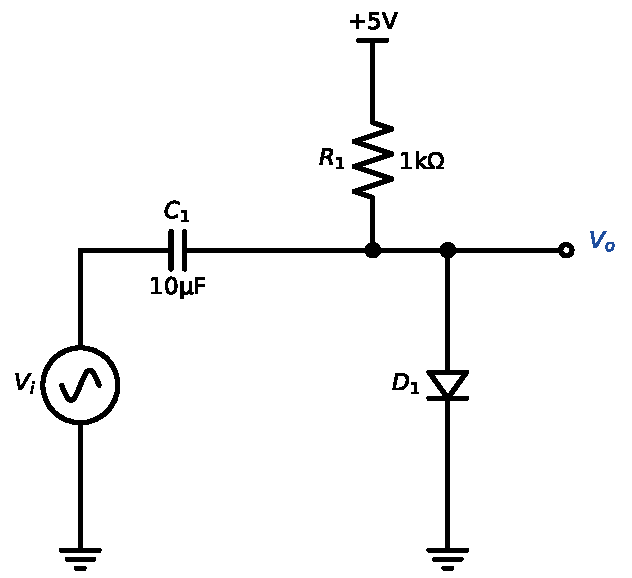
\includegraphics[width=0.9\linewidth,height=5cm,keepaspectratio]{p08_circuit}\end{center}
\solstep{1}{DC operating point}DC rules (tool T3): $v_i = 0$ and every capacitor is open ($C_{1}$). With the exponential model the diode voltage is unknown, so first reduce the rest of the circuit to what the diode sees: a Thevenin source. Remove the diode and solve the circuit (Lecture 2 KCL): the open-circuit voltage across it is $V_{th} = 5\,\mathrm{V}$. Short the diode instead: the current is $I_{sc} = 5\,\mathrm{m}\mathrm{A}$. So $R_{th} = \frac{V_{th}}{I_{sc}} = 1\,\mathrm{k}\Omega$.

Two equations, two unknowns: the circuit gives $I_D = \frac{V_{th}-V_D}{R_{th}}$ and the diode gives $V_D = nV_T\ln\frac{I_D}{I_S}$ (tool T1, $n=1.8$, $V_T = 25$\,mV, $I_S = 2.6\,\mathrm{n}\mathrm{A}$). Solve by iteration: guess $V_D = 0.7$\,V, compute $I_D$, update $V_D$, repeat until nothing changes:\begin{center}\renewcommand{\arraystretch}{1.35}
\begin{tabular}{cccc}
\toprule
step & $V_D$ used (V) & circuit $\Rightarrow I_D$ & diode $\Rightarrow$ new $V_D$ (V) \\
\midrule
1 & $0.7$ & $I_D = \frac{5 - 0.7}{1000} = 4.3\,\mathrm{m}\mathrm{A}$ & $0.6443$ \\
2 & $0.6443$ & $I_D = \frac{5 - 0.6443}{1000} = 4.36\,\mathrm{m}\mathrm{A}$ & $0.6449$ \\
3 & $0.6449$ & $I_D = \frac{5 - 0.6449}{1000} = 4.36\,\mathrm{m}\mathrm{A}$ & $0.6449$ \\
4 & $0.6449$ & $I_D = \frac{5 - 0.6449}{1000} = 4.36\,\mathrm{m}\mathrm{A}$ & $0.6449$ \\
5 & $0.6449$ & $I_D = \frac{5 - 0.6449}{1000} = 4.36\,\mathrm{m}\mathrm{A}$ & $0.6449$ \\
\bottomrule
\end{tabular}\end{center}
Converged: $V_D = 0.6449$\,V, $I_D = 4.36\,\mathrm{m}\mathrm{A}$. With this $V_D$ the rest of the DC circuit gives $V_{o,dc} = 645\,\mathrm{m}\mathrm{V}$.\[
\boxed{V_{o,dc} = 645\,\mathrm{m}\mathrm{V}}
\]

\solstep{2}{Small-signal resistance}$r_{d} = \frac{nV_T}{I_D} = \frac{1.8\times 25\,\mathrm{mV}}{4.36\,\mathrm{m}\mathrm{A}} = 10.3\,\Omega$ (tool T3). For the AC analysis the diode is just this resistor.
\solstep{3}{AC circuit}Set every DC supply to zero: each supply rail becomes AC ground. Replace every capacitor by $\frac{1}{sC}$ and every inductor by $sL$.
AC equivalent circuit (nodes named for the next step):
\begin{center}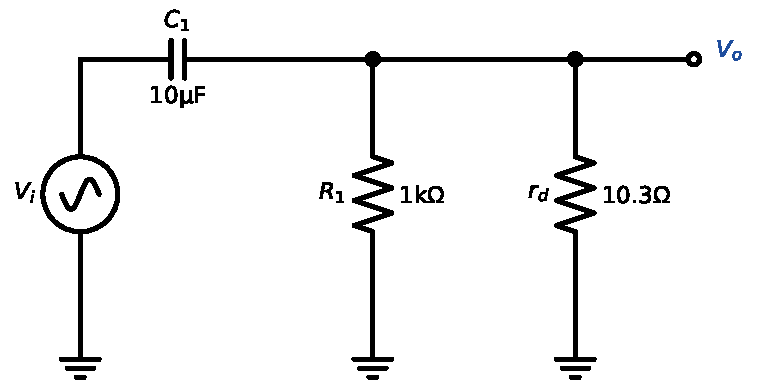
\includegraphics[width=0.95\linewidth,height=5.2cm,keepaspectratio]{p08_ac}\end{center}

\solstep{4}{Transfer function by a chain of dividers}Walk from the input to the output through the named nodes: $V_{i} \to V_{o}$. There is a single link, so $H(s)$ is just one voltage divider (tool T2).
Impedances seen \emph{looking right} from a node (everything from that node to ground, excluding what is on its left). Compute them from the far right toward the input:
\begin{align*}
Z_{o} &= R_{1} \parallel r_d = 10.2
\end{align*}

Now each link. {\small (Algebra tip: to simplify a fraction that contains fractions, multiply its top and bottom by every inner denominator; then divide top and bottom by the leading coefficient of the denominator so that it starts with a plain $s^n$.)}
\begin{align*}
\frac{V_{o}}{V_{i}} &= \frac{Z_{o}}{\frac{1}{sC_{1}} + Z_{o}} = \dfrac{s}{s + 9780}
\end{align*}
So:\[
H(s) = \dfrac{s}{s + 9780}
\]

\solstep{5}{Standard (Bode-ready) form}Find the roots. Every root $s=-p$ of the denominator is a \emph{pole}, every root $s=-z$ of the numerator is a \emph{zero}; $|p|$ and $|z|$ are the corner frequencies (rad/s).
\begin{itemize}[leftmargin=*,itemsep=2pt]
\item Numerator: it has the factor $s$ $\Rightarrow$ 1 zero at $s=0$.
\item Denominator: $s + 9780$; $s + 9780 = 0 \Rightarrow s = -9780$.
\end{itemize}

Factored form (leading coefficient in front):
\[
H(s) = 1\,\dfrac{s}{(s+9780)}
\]

Bode-ready form: rewrite every $(s+p) = p\left(1+\frac{s}{p}\right)$ and $(s+z) = z\left(1+\frac{s}{z}\right)$, and collect all constants into $K$. Each $s$ in the numerator is paired with one of the \emph{lowest} poles as $\frac{s}{s+p}$ (that factor is $\approx 1$ above $p$). Then every factor except $K$ is $\approx 1$ inside the pass-band:
\[
H(s) = 1\,\dfrac{s}{s+2\pi\cdot 1.56\mathrm{k}},\qquad K = 1
\]

\begin{center}\renewcommand{\arraystretch}{1.35}
\begin{tabular}{cccc}
\toprule
type & $\omega_c$ (rad/s) & $f_c=\omega_c/2\pi$ & slope change \\
\midrule
pole & $9780$ & 1.56 kHz & $-20$ dB/dec \\
\bottomrule
\end{tabular}\end{center}

\solstep{6}{Magnitude Bode plot}Below every corner $|H(s)|\approx 1.02\times 10^{-4}\,s$, so the plot starts with a slope of $+20$\,dB/dec. Then, moving right, each pole bends the line down by 20\,dB/dec and each zero bends it up by 20\,dB/dec (tool T6):
\begin{center}\renewcommand{\arraystretch}{1.35}
\begin{tabular}{lcl}
\toprule
frequency range & slope & asymptote level \\
\midrule
$f<$ 1.56 kHz & $+20$ dB/dec & 0 dB at end \\
$f>$ 1.56 kHz & $0$ dB/dec (flat) & 0 dB at start \\
\bottomrule
\end{tabular}\end{center}

The flat (pass-band) level is $20\log_{10}|K| = 20\log_{10}1 = 0$\,dB.
\begin{center}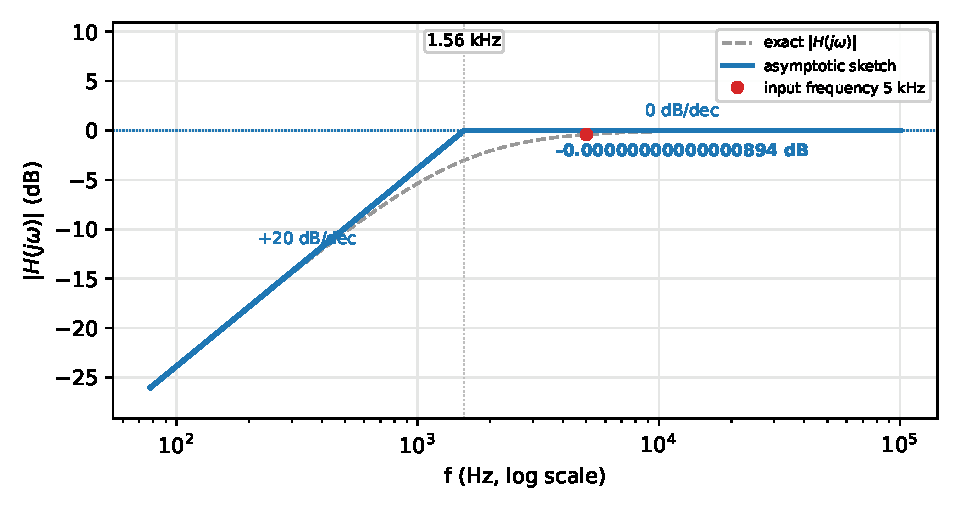
\includegraphics[width=0.78\linewidth,height=6.5cm,keepaspectratio]{p08_bode}\end{center}

{\small Blue: the straight-line sketch you are expected to draw. Dashed grey: the exact curve (about 3\,dB below the corner of an isolated pole). Red dot: the input frequency of Step 7.}
\solstep{7}{Total output (DC + AC)}The input is $V_i(t) = 0.002\sin\left(2\pi\cdot 5000\,t\right)$, so $\omega_{in} = 2\pi\cdot 5000 = 31400$\,rad/s. Put $s=j\omega_{in}$ in each factor (tool T5): magnitudes multiply, angles add.
{\small Rules: $\left|\frac{s}{s+p}\right| = \frac{\omega}{\sqrt{\omega^2+p^2}}$, $\angle = \frac{\pi}{2}-\tan^{-1}\frac{\omega}{p}$;\quad $\left|\frac{1}{1+s/p}\right| = \frac{1}{\sqrt{1+(\omega/p)^2}}$, $\angle = -\tan^{-1}\frac{\omega}{p}$;\quad $\left|1+\frac{s}{z}\right| = \sqrt{1+(\omega/z)^2}$, $\angle = \tan^{-1}\frac{\omega}{z}$;\quad a negative $K$ adds $-\pi$.}
\begin{center}\renewcommand{\arraystretch}{1.35}
\begin{tabular}{ccc}
\toprule
factor & magnitude & angle (rad) \\
\midrule
$1$ & $1$ & $0$ \\
$\rule[-1.1em]{0pt}{2.8em}\dfrac{s}{s+2\pi\cdot 1.56\mathrm{k}}$ & $0.9548$ & $0.302$ \\
\textbf{total} & $\mathbf{0.9548}$ (product) & $\mathbf{0.302}$ (sum) \\
\bottomrule
\end{tabular}\end{center}

\begin{align*}
|H(j\omega_{in})| &= 0.955, \qquad \angle H(j\omega_{in}) = 0.302\ \mathrm{rad} \\
v_{o,ac}(t) &= 0.955\times 0.002\,\sin\left(2\pi\cdot 5000\,t + 0.302\right) = 0.00191\,\sin\left(2\pi\cdot 5000\,t + 0.302\right)
\end{align*}

Add the DC part from Step 2 (superposition):
\[
\boxed{V_o(t) = 0.645 + 0.00191\,\sin\left(2\pi\cdot 5000\,t + 0.302\right)\ \mathrm{V}}
\]
 Check the small-signal assumption: the AC voltage across the diode has amplitude about $1.91\,\mathrm{m}\mathrm{V}$, well below $nV_T = 45\,\mathrm{m}\mathrm{V}$ \checkmark.
\begin{ansbox}
$H(s) = 1\,\dfrac{s}{s+2\pi\cdot 1.56\mathrm{k}}$\quad (corners: 1.56 kHz)\\[4pt]
$V_o(t) = 0.645 + 0.00191\,\sin\left(2\pi\cdot 5000\,t + 0.302\right)\ \mathrm{V}$
\end{ansbox}

\newpage
\subsection*{Solution 3D.9 \hfill Medium}
\begin{center}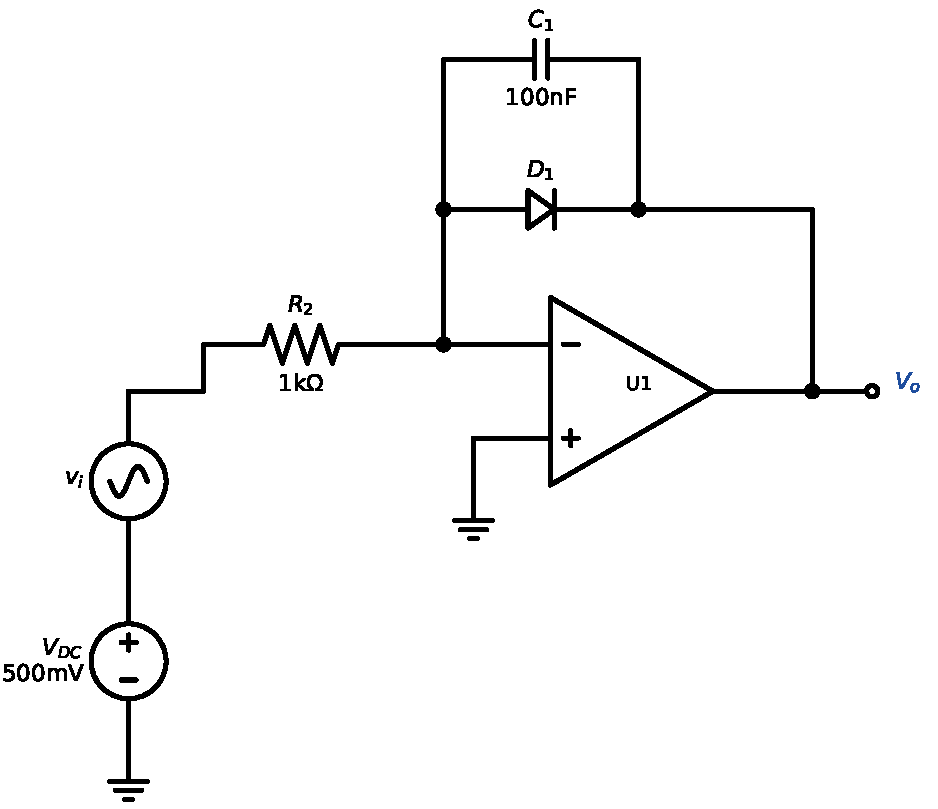
\includegraphics[width=0.9\linewidth,height=5cm,keepaspectratio]{p09_circuit}\end{center}
\solstep{1}{DC operating point}DC rules (tool T3): $v_i = 0$, so the input is just $V_{DC} = 500\,\mathrm{m}\mathrm{V}$; capacitors are open. The op-amp has negative feedback, so $V_- = V_+ = 0$ (virtual ground) and no current enters its inputs. The input current $\frac{V_{DC} - 0}{R_{2}} = 500\,\mu \mathrm{A}$ cannot enter the op-amp: all of it flows through the diode, $I_D = 500\,\mu \mathrm{A}$. Exponential model (tool T1):\[
V_D = nV_T\ln\frac{I_D}{I_S} = 1.8\times 0.025\times\ln\frac{5\times 10^{-4}}{2.6\times 10^{-9}} = 548\,\mathrm{m}\mathrm{V}
\]
 The diode current flows from the $-$ input (at 0\,V) toward the output, so the output sits $V_D$ below it:\[
V_{o,dc} = -(V_D) = -548\,\mathrm{m}\mathrm{V}
\]
\[
\boxed{V_{o,dc} = -548\,\mathrm{m}\mathrm{V}}
\]

\solstep{2}{Small-signal resistance}$r_d = \frac{nV_T}{I_D} = \frac{1.8\times 25\,\mathrm{mV}}{500\,\mu \mathrm{A}} = 90\,\Omega$ (tool T3). For the AC analysis the diode is just this resistor, and $V_{DC}$ is replaced by a short (AC ground).
\solstep{3}{AC circuit}\begin{center}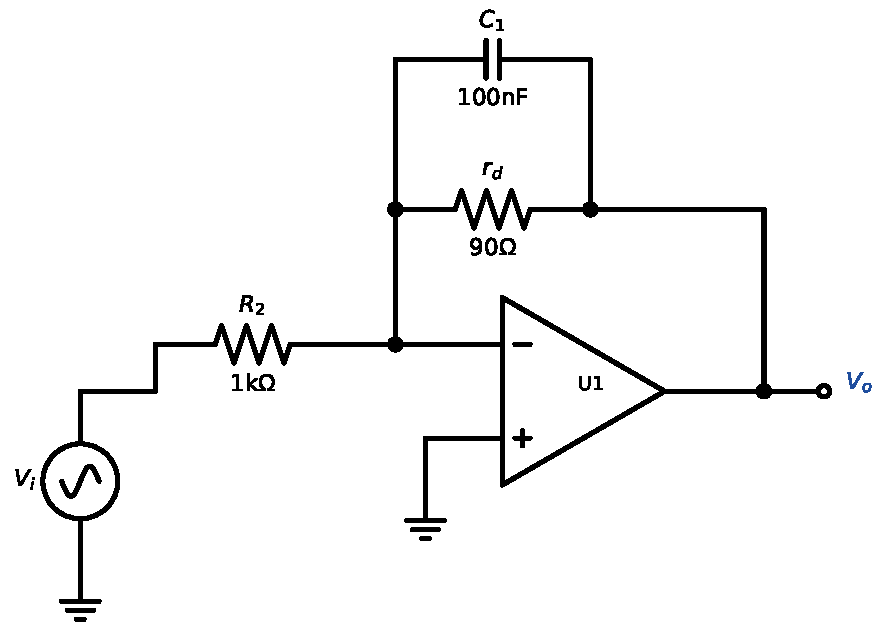
\includegraphics[width=0.9\linewidth,height=5cm,keepaspectratio]{p09_ac}\end{center}

\solstep{4}{Transfer function}\textbf{Block 1 (U1).} Inverting block: the $+$ input is grounded, so $V_- = V_+ = 0$ (virtual ground). The current $\frac{V_{i} - 0}{R_{2}}$ through $R_{2}$ cannot enter the op-amp, so all of it flows through $Z_{f1}$: $V_{o} = 0 - Z_{f1}\cdot\frac{V_{i}}{R_{2}}$.\begin{align*}
Z_{f1} &= r_d \parallel \frac{1}{sC_{1}} = \dfrac{10^{7}}{s + 1.11\times 10^{5}}
\end{align*}
\[
\frac{V_{o}}{V_{i}} = -\frac{Z_{f1}}{R_{2}} = \dfrac{-10000}{s + 1.11\times 10^{5}}
\]
So:\[
H(s) = \dfrac{-10000}{s + 1.11\times 10^{5}}
\]

\solstep{5}{Standard (Bode-ready) form}Find the roots. Every root $s=-p$ of the denominator is a \emph{pole}, every root $s=-z$ of the numerator is a \emph{zero}; $|p|$ and $|z|$ are the corner frequencies (rad/s).
\begin{itemize}[leftmargin=*,itemsep=2pt]
\item Denominator: $s + 1.11\times 10^{5}$; $s + 1.11\times 10^{5} = 0 \Rightarrow s = -1.11\times 10^{5}$.
\end{itemize}

Factored form (leading coefficient in front):
\[
H(s) = -10000\,\dfrac{1}{(s+1.11\times 10^{5})}
\]

Bode-ready form: rewrite every $(s+p) = p\left(1+\frac{s}{p}\right)$ and $(s+z) = z\left(1+\frac{s}{z}\right)$, and collect all constants into $K$. Then every factor except $K$ is $\approx 1$ inside the pass-band:
\[
H(s) = -0.09\,\dfrac{1}{1+\dfrac{s}{2\pi\cdot 17.7\mathrm{k}}},\qquad K = -0.09
\]

\begin{center}\renewcommand{\arraystretch}{1.35}
\begin{tabular}{cccc}
\toprule
type & $\omega_c$ (rad/s) & $f_c=\omega_c/2\pi$ & slope change \\
\midrule
pole & $1.11\times 10^{5}$ & 17.7 kHz & $-20$ dB/dec \\
\bottomrule
\end{tabular}\end{center}

\solstep{6}{Magnitude Bode plot}Below every corner, all factors are $\approx$ constant: $|H| \approx 0.09$ $= -20.9$\,dB (flat, 0 dB/dec). Then, moving right, each pole bends the line down by 20\,dB/dec and each zero bends it up by 20\,dB/dec (tool T6):
\begin{center}\renewcommand{\arraystretch}{1.35}
\begin{tabular}{lcl}
\toprule
frequency range & slope & asymptote level \\
\midrule
$f<$ 17.7 kHz & $0$ dB/dec (flat) & -20.9 dB at end \\
$f>$ 17.7 kHz & $-20$ dB/dec & -20.9 dB at start \\
\bottomrule
\end{tabular}\end{center}

The flat (pass-band) level is $20\log_{10}|K| = 20\log_{10}0.09 = -20.9$\,dB.
\begin{center}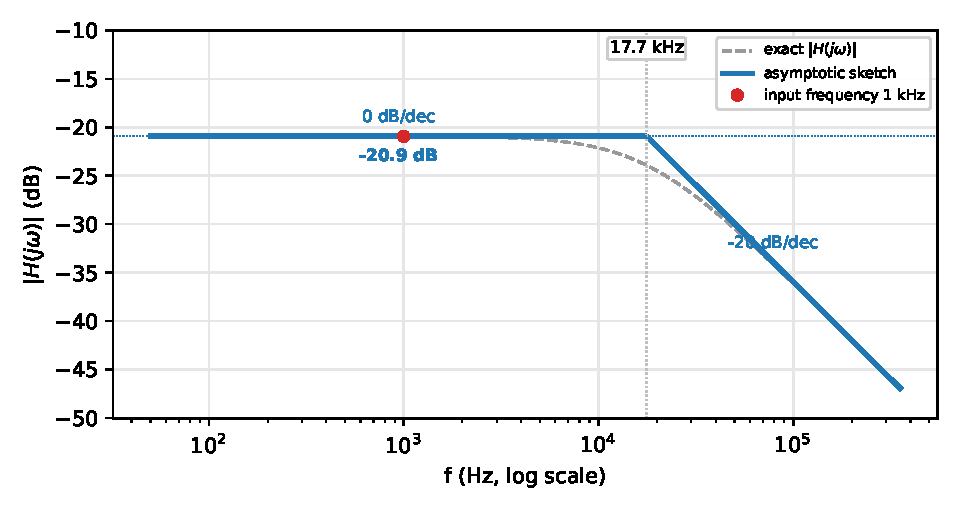
\includegraphics[width=0.78\linewidth,height=6.5cm,keepaspectratio]{p09_bode}\end{center}

{\small Blue: the straight-line sketch you are expected to draw. Dashed grey: the exact curve (about 3\,dB below the corner of an isolated pole). Red dot: the input frequency of Step 7.}
\solstep{7}{Total output (DC + AC)}The input is $V_i(t) = 0.05\sin\left(2\pi\cdot 1000\,t\right)$, so $\omega_{in} = 2\pi\cdot 1000 = 6280$\,rad/s. Put $s=j\omega_{in}$ in each factor (tool T5): magnitudes multiply, angles add.
{\small Rules: $\left|\frac{s}{s+p}\right| = \frac{\omega}{\sqrt{\omega^2+p^2}}$, $\angle = \frac{\pi}{2}-\tan^{-1}\frac{\omega}{p}$;\quad $\left|\frac{1}{1+s/p}\right| = \frac{1}{\sqrt{1+(\omega/p)^2}}$, $\angle = -\tan^{-1}\frac{\omega}{p}$;\quad $\left|1+\frac{s}{z}\right| = \sqrt{1+(\omega/z)^2}$, $\angle = \tan^{-1}\frac{\omega}{z}$;\quad a negative $K$ adds $-\pi$.}
\begin{center}\renewcommand{\arraystretch}{1.35}
\begin{tabular}{ccc}
\toprule
factor & magnitude & angle (rad) \\
\midrule
$-0.09$ & $0.09$ & $-3.14$ \\
$\rule[-1.7em]{0pt}{4em}\dfrac{1}{1+\dfrac{s}{2\pi\cdot 17.7\mathrm{k}}}$ & $0.9984$ & $-0.0565$ \\
\textbf{total} & $\mathbf{0.08986}$ (product) & $\mathbf{-3.2}$ (sum) \\
\bottomrule
\end{tabular}\end{center}

\begin{align*}
|H(j\omega_{in})| &= 0.0899, \qquad \angle H(j\omega_{in}) = -3.2\ \mathrm{rad} \\
v_{o,ac}(t) &= 0.0899\times 0.05\,\sin\left(2\pi\cdot 1000\,t - 3.2\right) = 0.00449\,\sin\left(2\pi\cdot 1000\,t - 3.2\right)
\end{align*}

Add the DC part from Step 2 (superposition):
\[
\boxed{V_o(t) = -0.548 + 0.00449\,\sin\left(2\pi\cdot 1000\,t - 3.2\right)\ \mathrm{V}}
\]
 Check the small-signal assumption: the AC voltage across the diode has amplitude about $4.49\,\mathrm{m}\mathrm{V}$, well below $nV_T = 45\,\mathrm{m}\mathrm{V}$ \checkmark.
\begin{ansbox}
$H(s) = -0.09\,\dfrac{1}{1+\dfrac{s}{2\pi\cdot 17.7\mathrm{k}}}$\quad (corners: 17.7 kHz)\\[4pt]
$V_o(t) = -0.548 + 0.00449\,\sin\left(2\pi\cdot 1000\,t - 3.2\right)\ \mathrm{V}$
\end{ansbox}

\newpage
\subsection*{Solution 3D.10 \hfill Medium}
\begin{center}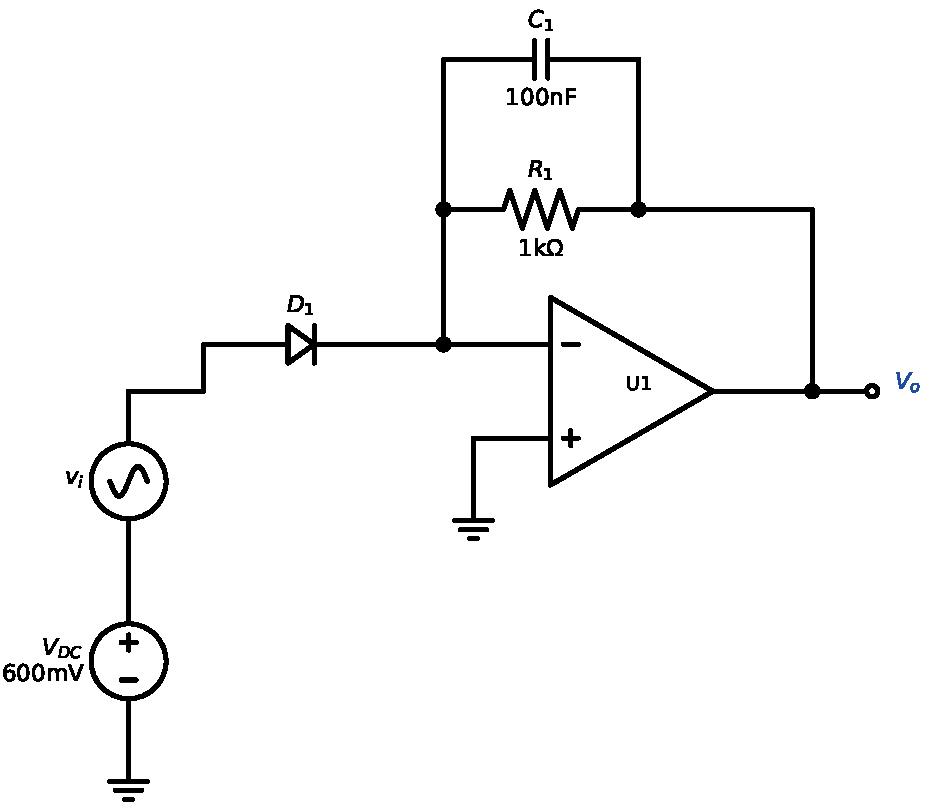
\includegraphics[width=0.9\linewidth,height=5cm,keepaspectratio]{p10_circuit}\end{center}
\solstep{1}{DC operating point}DC rules (tool T3): $v_i = 0$, so the input is just $V_{DC} = 600\,\mathrm{m}\mathrm{V}$; capacitors are open. The op-amp has negative feedback, so $V_- = V_+ = 0$ (virtual ground) and no current enters its inputs. The diode sits between $V_{DC}$ and the virtual ground, so $V_D = V_{DC} = 600\,\mathrm{m}\mathrm{V}$ and the exponential model (tool T1) gives\[
I_D = I_S\,e^{V_D/nV_T} = 2.6\,\mathrm{n}\mathrm{A}\times \exp\left(\frac{0.6}{1.8\times 0.025}\right) = 1.61\,\mathrm{m}\mathrm{A}
\]
 All of $I_D$ continues through the feedback resistor $R_{1}$ (the capacitor is open), so\[
V_{o,dc} = 0 - R_{1}I_D = -1000\times0.001605 = -1.61\,\mathrm{V}
\]
\[
\boxed{V_{o,dc} = -1.61\,\mathrm{V}}
\]

\solstep{2}{Small-signal resistance}$r_d = \frac{nV_T}{I_D} = \frac{1.8\times 25\,\mathrm{mV}}{1.61\,\mathrm{m}\mathrm{A}} = 28\,\Omega$ (tool T3). For the AC analysis the diode is just this resistor, and $V_{DC}$ is replaced by a short (AC ground).
\solstep{3}{AC circuit}\begin{center}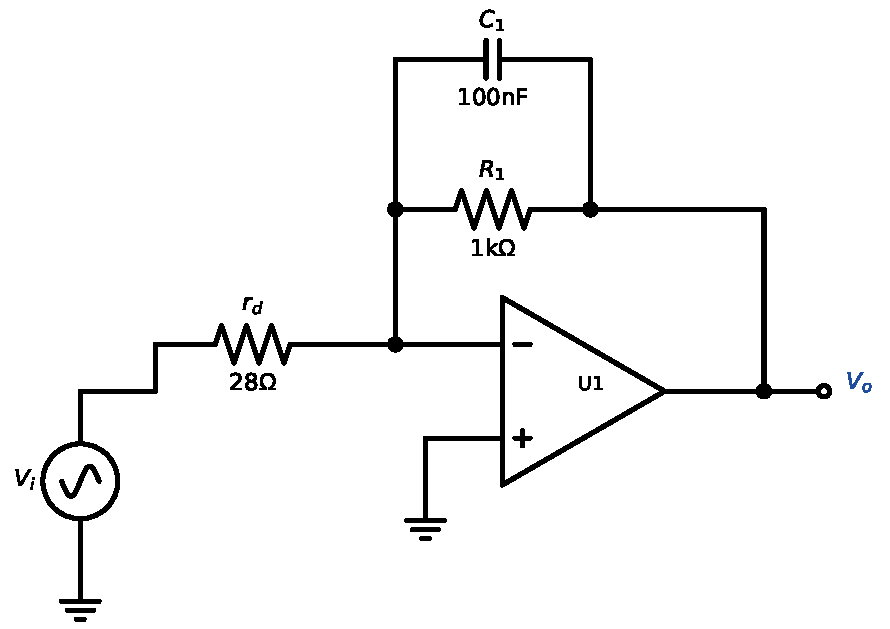
\includegraphics[width=0.9\linewidth,height=5cm,keepaspectratio]{p10_ac}\end{center}

\solstep{4}{Transfer function}\textbf{Block 1 (U1).} Inverting block: the $+$ input is grounded, so $V_- = V_+ = 0$ (virtual ground). The current $\frac{V_{i} - 0}{r_d}$ through $r_d$ cannot enter the op-amp, so all of it flows through $Z_{f1}$: $V_{o} = 0 - Z_{f1}\cdot\frac{V_{i}}{r_d}$.\begin{align*}
Z_{f1} &= R_{1} \parallel \frac{1}{sC_{1}} = \dfrac{10^{7}}{s + 10000}
\end{align*}
\[
\frac{V_{o}}{V_{i}} = -\frac{Z_{f1}}{r_d} = \dfrac{-3.57\times 10^{5}}{s + 10000}
\]
So:\[
H(s) = \dfrac{-3.57\times 10^{5}}{s + 10000}
\]

\solstep{5}{Standard (Bode-ready) form}Find the roots. Every root $s=-p$ of the denominator is a \emph{pole}, every root $s=-z$ of the numerator is a \emph{zero}; $|p|$ and $|z|$ are the corner frequencies (rad/s).
\begin{itemize}[leftmargin=*,itemsep=2pt]
\item Denominator: $s + 10000$; $s + 10000 = 0 \Rightarrow s = -10000$.
\end{itemize}

Factored form (leading coefficient in front):
\[
H(s) = -3.57\times 10^{5}\,\dfrac{1}{(s+10000)}
\]

Bode-ready form: rewrite every $(s+p) = p\left(1+\frac{s}{p}\right)$ and $(s+z) = z\left(1+\frac{s}{z}\right)$, and collect all constants into $K$. Then every factor except $K$ is $\approx 1$ inside the pass-band:
\[
H(s) = -35.7\,\dfrac{1}{1+\dfrac{s}{2\pi\cdot 1.59\mathrm{k}}},\qquad K = -35.7
\]

\begin{center}\renewcommand{\arraystretch}{1.35}
\begin{tabular}{cccc}
\toprule
type & $\omega_c$ (rad/s) & $f_c=\omega_c/2\pi$ & slope change \\
\midrule
pole & $10000$ & 1.59 kHz & $-20$ dB/dec \\
\bottomrule
\end{tabular}\end{center}

\solstep{6}{Magnitude Bode plot}Below every corner, all factors are $\approx$ constant: $|H| \approx 35.7$ $= 31$\,dB (flat, 0 dB/dec). Then, moving right, each pole bends the line down by 20\,dB/dec and each zero bends it up by 20\,dB/dec (tool T6):
\begin{center}\renewcommand{\arraystretch}{1.35}
\begin{tabular}{lcl}
\toprule
frequency range & slope & asymptote level \\
\midrule
$f<$ 1.59 kHz & $0$ dB/dec (flat) & 31 dB at end \\
$f>$ 1.59 kHz & $-20$ dB/dec & 31 dB at start \\
\bottomrule
\end{tabular}\end{center}

The flat (pass-band) level is $20\log_{10}|K| = 20\log_{10}35.7 = 31$\,dB.
\begin{center}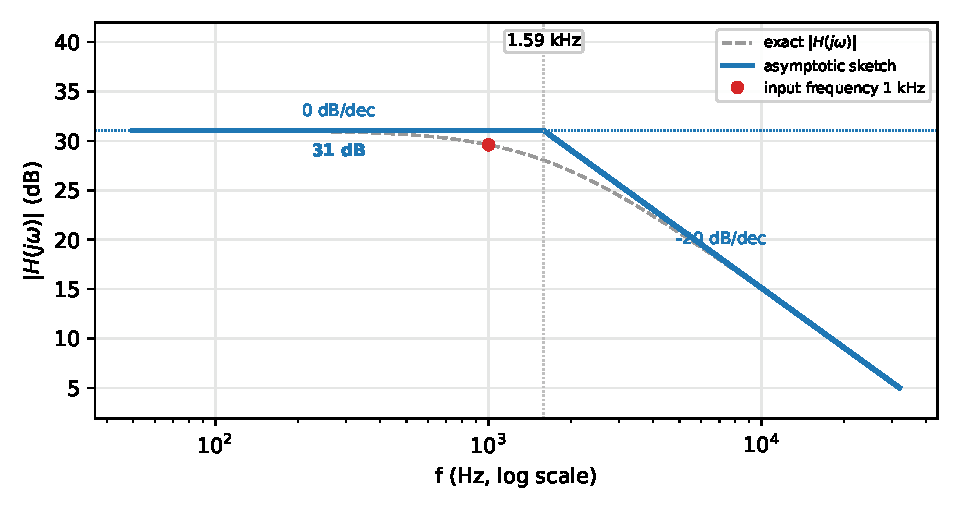
\includegraphics[width=0.78\linewidth,height=6.5cm,keepaspectratio]{p10_bode}\end{center}

{\small Blue: the straight-line sketch you are expected to draw. Dashed grey: the exact curve (about 3\,dB below the corner of an isolated pole). Red dot: the input frequency of Step 7.}
\solstep{7}{Total output (DC + AC)}The input is $V_i(t) = 0.003\sin\left(2\pi\cdot 1000\,t\right)$, so $\omega_{in} = 2\pi\cdot 1000 = 6280$\,rad/s. Put $s=j\omega_{in}$ in each factor (tool T5): magnitudes multiply, angles add.
{\small Rules: $\left|\frac{s}{s+p}\right| = \frac{\omega}{\sqrt{\omega^2+p^2}}$, $\angle = \frac{\pi}{2}-\tan^{-1}\frac{\omega}{p}$;\quad $\left|\frac{1}{1+s/p}\right| = \frac{1}{\sqrt{1+(\omega/p)^2}}$, $\angle = -\tan^{-1}\frac{\omega}{p}$;\quad $\left|1+\frac{s}{z}\right| = \sqrt{1+(\omega/z)^2}$, $\angle = \tan^{-1}\frac{\omega}{z}$;\quad a negative $K$ adds $-\pi$.}
\begin{center}\renewcommand{\arraystretch}{1.35}
\begin{tabular}{ccc}
\toprule
factor & magnitude & angle (rad) \\
\midrule
$-35.7$ & $35.67$ & $-3.14$ \\
$\rule[-1.7em]{0pt}{4em}\dfrac{1}{1+\dfrac{s}{2\pi\cdot 1.59\mathrm{k}}}$ & $0.8467$ & $-0.561$ \\
\textbf{total} & $\mathbf{30.21}$ (product) & $\mathbf{-3.7}$ (sum) \\
\bottomrule
\end{tabular}\end{center}

\begin{align*}
|H(j\omega_{in})| &= 30.2, \qquad \angle H(j\omega_{in}) = -3.7\ \mathrm{rad} \\
v_{o,ac}(t) &= 30.2\times 0.003\,\sin\left(2\pi\cdot 1000\,t - 3.7\right) = 0.0906\,\sin\left(2\pi\cdot 1000\,t - 3.7\right)
\end{align*}

Add the DC part from Step 2 (superposition):
\[
\boxed{V_o(t) = -1.61 + 0.0906\,\sin\left(2\pi\cdot 1000\,t - 3.7\right)\ \mathrm{V}}
\]
 Check the small-signal assumption: the AC voltage across the diode has amplitude about $3\,\mathrm{m}\mathrm{V}$, well below $nV_T = 45\,\mathrm{m}\mathrm{V}$ \checkmark.
\begin{ansbox}
$H(s) = -35.7\,\dfrac{1}{1+\dfrac{s}{2\pi\cdot 1.59\mathrm{k}}}$\quad (corners: 1.59 kHz)\\[4pt]
$V_o(t) = -1.61 + 0.0906\,\sin\left(2\pi\cdot 1000\,t - 3.7\right)\ \mathrm{V}$
\end{ansbox}

\newpage
\subsection*{Solution 3D.11 \hfill Medium}
\begin{center}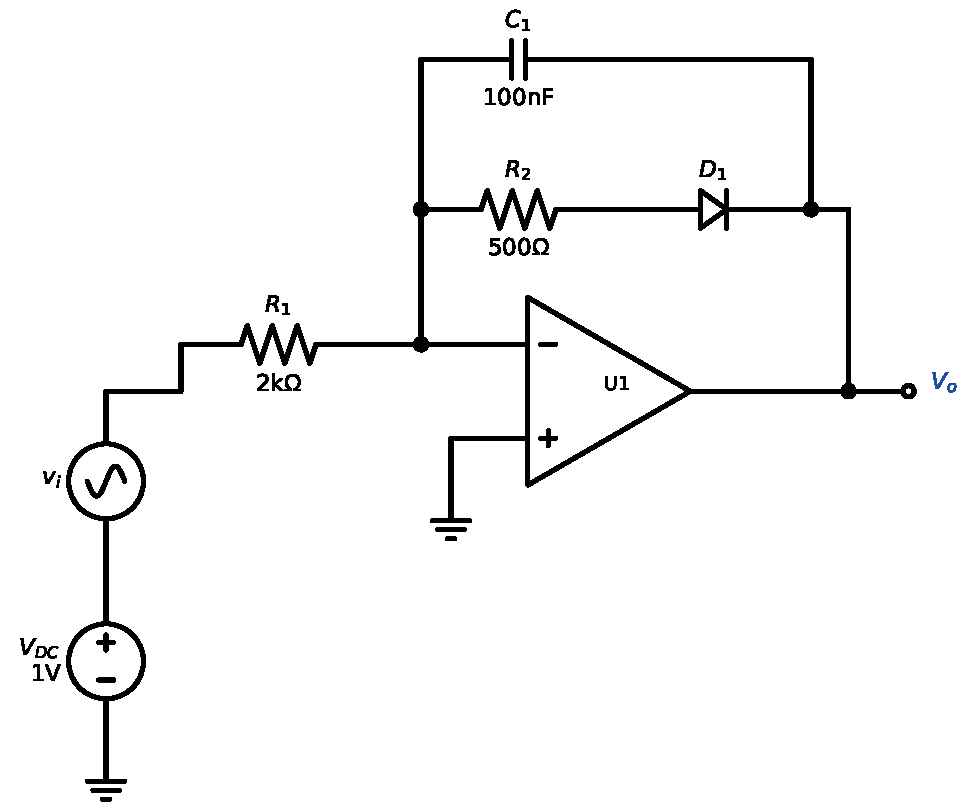
\includegraphics[width=0.9\linewidth,height=5cm,keepaspectratio]{p11_circuit}\end{center}
\solstep{1}{DC operating point}DC rules (tool T3): $v_i = 0$, so the input is just $V_{DC} = 1\,\mathrm{V}$; capacitors are open. The op-amp has negative feedback, so $V_- = V_+ = 0$ (virtual ground) and no current enters its inputs. The input current $\frac{V_{DC} - 0}{R_{1}} = 500\,\mu \mathrm{A}$ cannot enter the op-amp: all of it flows through the diode, $I_D = 500\,\mu \mathrm{A}$. Constant-voltage-drop model: $V_D = 0.7$\,V. The diode current flows from the $-$ input (at 0\,V) toward the output, so the output sits $V_D + R_{2}I_D$ below it:\[
V_{o,dc} = -(V_D + R_{2}I_D) = -950\,\mathrm{m}\mathrm{V}
\]
\[
\boxed{V_{o,dc} = -950\,\mathrm{m}\mathrm{V}}
\]

\solstep{2}{Small-signal resistance}$r_d = \frac{nV_T}{I_D} = \frac{1.8\times 25\,\mathrm{mV}}{500\,\mu \mathrm{A}} = 90\,\Omega$ (tool T3). For the AC analysis the diode is just this resistor, and $V_{DC}$ is replaced by a short (AC ground).
\solstep{3}{AC circuit}\begin{center}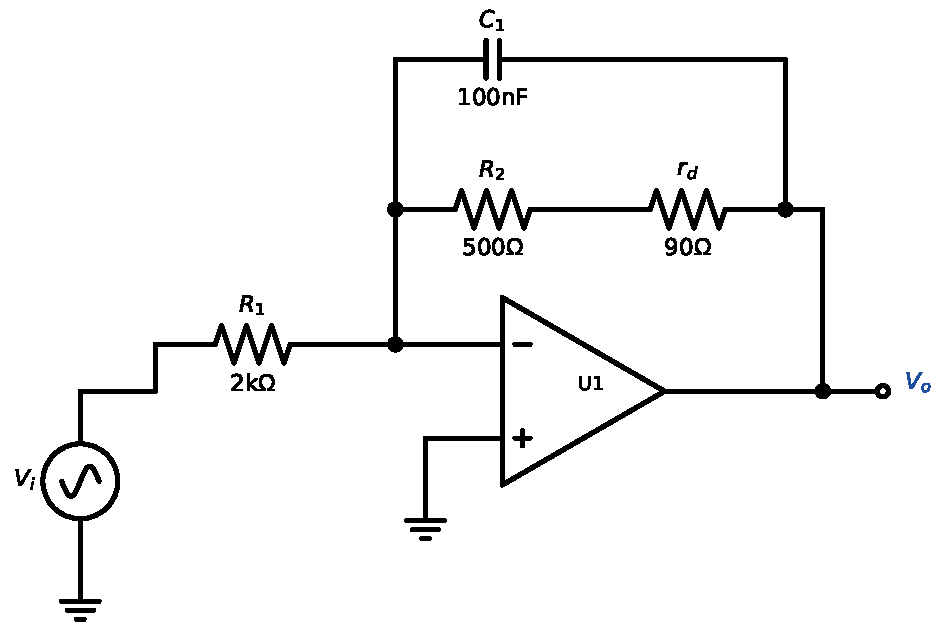
\includegraphics[width=0.9\linewidth,height=5cm,keepaspectratio]{p11_ac}\end{center}

\solstep{4}{Transfer function}\textbf{Block 1 (U1).} Inverting block: the $+$ input is grounded, so $V_- = V_+ = 0$ (virtual ground). The current $\frac{V_{i} - 0}{R_{1}}$ through $R_{1}$ cannot enter the op-amp, so all of it flows through $Z_{f1}$: $V_{o} = 0 - Z_{f1}\cdot\frac{V_{i}}{R_{1}}$.\begin{align*}
Z_{f1} &= \left(R_{2} + r_d\right) \parallel \frac{1}{sC_{1}} = \dfrac{10^{7}}{s + 16900}
\end{align*}
\[
\frac{V_{o}}{V_{i}} = -\frac{Z_{f1}}{R_{1}} = \dfrac{-5000}{s + 16900}
\]
So:\[
H(s) = \dfrac{-5000}{s + 16900}
\]

\solstep{5}{Standard (Bode-ready) form}Find the roots. Every root $s=-p$ of the denominator is a \emph{pole}, every root $s=-z$ of the numerator is a \emph{zero}; $|p|$ and $|z|$ are the corner frequencies (rad/s).
\begin{itemize}[leftmargin=*,itemsep=2pt]
\item Denominator: $s + 16900$; $s + 16900 = 0 \Rightarrow s = -16900$.
\end{itemize}

Factored form (leading coefficient in front):
\[
H(s) = -5000\,\dfrac{1}{(s+16900)}
\]

Bode-ready form: rewrite every $(s+p) = p\left(1+\frac{s}{p}\right)$ and $(s+z) = z\left(1+\frac{s}{z}\right)$, and collect all constants into $K$. Then every factor except $K$ is $\approx 1$ inside the pass-band:
\[
H(s) = -0.295\,\dfrac{1}{1+\dfrac{s}{2\pi\cdot 2.7\mathrm{k}}},\qquad K = -0.295
\]

\begin{center}\renewcommand{\arraystretch}{1.35}
\begin{tabular}{cccc}
\toprule
type & $\omega_c$ (rad/s) & $f_c=\omega_c/2\pi$ & slope change \\
\midrule
pole & $16900$ & 2.7 kHz & $-20$ dB/dec \\
\bottomrule
\end{tabular}\end{center}

\solstep{6}{Magnitude Bode plot}Below every corner, all factors are $\approx$ constant: $|H| \approx 0.295$ $= -10.6$\,dB (flat, 0 dB/dec). Then, moving right, each pole bends the line down by 20\,dB/dec and each zero bends it up by 20\,dB/dec (tool T6):
\begin{center}\renewcommand{\arraystretch}{1.35}
\begin{tabular}{lcl}
\toprule
frequency range & slope & asymptote level \\
\midrule
$f<$ 2.7 kHz & $0$ dB/dec (flat) & -10.6 dB at end \\
$f>$ 2.7 kHz & $-20$ dB/dec & -10.6 dB at start \\
\bottomrule
\end{tabular}\end{center}

The flat (pass-band) level is $20\log_{10}|K| = 20\log_{10}0.295 = -10.6$\,dB.
\begin{center}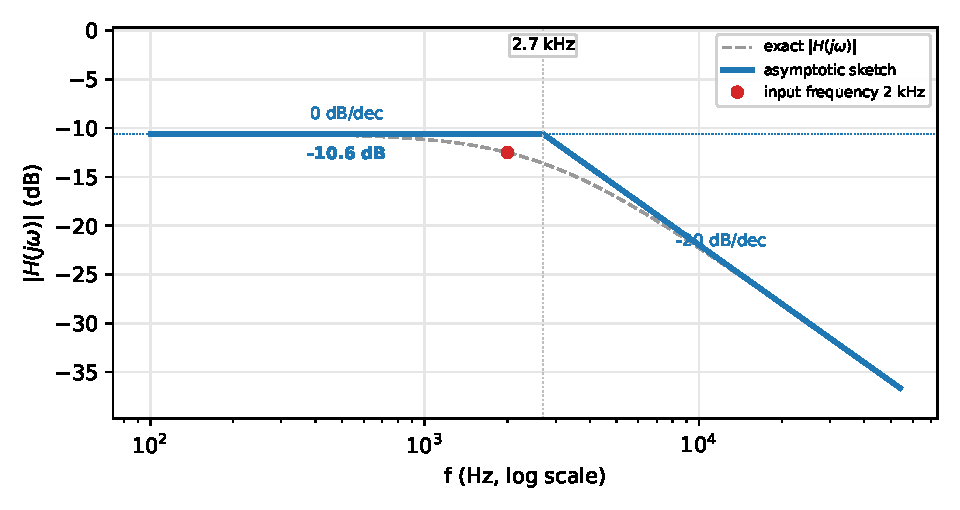
\includegraphics[width=0.78\linewidth,height=6.5cm,keepaspectratio]{p11_bode}\end{center}

{\small Blue: the straight-line sketch you are expected to draw. Dashed grey: the exact curve (about 3\,dB below the corner of an isolated pole). Red dot: the input frequency of Step 7.}
\solstep{7}{Total output (DC + AC)}The input is $V_i(t) = 0.05\sin\left(2\pi\cdot 2000\,t\right)$, so $\omega_{in} = 2\pi\cdot 2000 = 12600$\,rad/s. Put $s=j\omega_{in}$ in each factor (tool T5): magnitudes multiply, angles add.
{\small Rules: $\left|\frac{s}{s+p}\right| = \frac{\omega}{\sqrt{\omega^2+p^2}}$, $\angle = \frac{\pi}{2}-\tan^{-1}\frac{\omega}{p}$;\quad $\left|\frac{1}{1+s/p}\right| = \frac{1}{\sqrt{1+(\omega/p)^2}}$, $\angle = -\tan^{-1}\frac{\omega}{p}$;\quad $\left|1+\frac{s}{z}\right| = \sqrt{1+(\omega/z)^2}$, $\angle = \tan^{-1}\frac{\omega}{z}$;\quad a negative $K$ adds $-\pi$.}
\begin{center}\renewcommand{\arraystretch}{1.35}
\begin{tabular}{ccc}
\toprule
factor & magnitude & angle (rad) \\
\midrule
$-0.295$ & $0.295$ & $-3.14$ \\
$\rule[-1.7em]{0pt}{4em}\dfrac{1}{1+\dfrac{s}{2\pi\cdot 2.7\mathrm{k}}}$ & $0.8033$ & $-0.638$ \\
\textbf{total} & $\mathbf{0.237}$ (product) & $\mathbf{-3.78}$ (sum) \\
\bottomrule
\end{tabular}\end{center}

\begin{align*}
|H(j\omega_{in})| &= 0.237, \qquad \angle H(j\omega_{in}) = -3.78\ \mathrm{rad} \\
v_{o,ac}(t) &= 0.237\times 0.05\,\sin\left(2\pi\cdot 2000\,t - 3.78\right) = 0.0118\,\sin\left(2\pi\cdot 2000\,t - 3.78\right)
\end{align*}

Add the DC part from Step 2 (superposition):
\[
\boxed{V_o(t) = -0.95 + 0.0118\,\sin\left(2\pi\cdot 2000\,t - 3.78\right)\ \mathrm{V}}
\]
 Check the small-signal assumption: the AC voltage across the diode has amplitude about $1.81\,\mathrm{m}\mathrm{V}$, well below $nV_T = 45\,\mathrm{m}\mathrm{V}$ \checkmark.
\begin{ansbox}
$H(s) = -0.295\,\dfrac{1}{1+\dfrac{s}{2\pi\cdot 2.7\mathrm{k}}}$\quad (corners: 2.7 kHz)\\[4pt]
$V_o(t) = -0.95 + 0.0118\,\sin\left(2\pi\cdot 2000\,t - 3.78\right)\ \mathrm{V}$
\end{ansbox}

\newpage
\subsection*{Solution 3D.12 \hfill Medium}
\begin{center}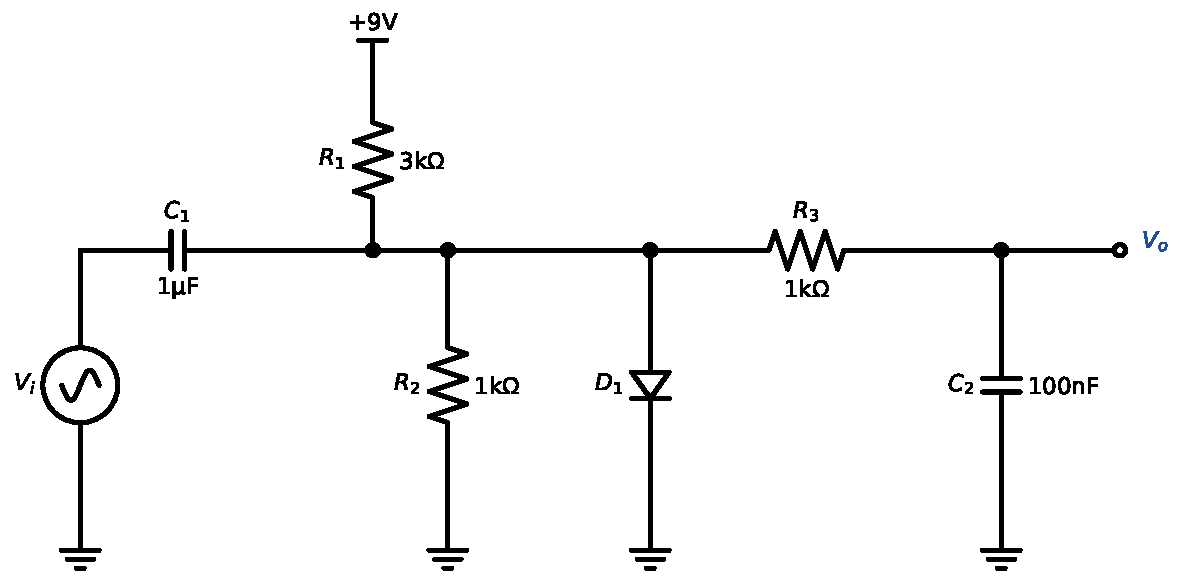
\includegraphics[width=0.9\linewidth,height=5cm,keepaspectratio]{p12_circuit}\end{center}
\solstep{1}{DC operating point}DC rules (tool T3): $v_i = 0$ and every capacitor is open ($C_{1}, C_{2}$). Assume the diode is ON (constant-voltage-drop model, $0.7$\,V) and solve the DC circuit:

Replace $D_{1}$ ON: a $0.7$\,V source ($V_{1} - 0 = 0.7$) carrying an unknown current $I_{D_{1}}$ from anode to cathode.

Equations (KCL at every node that is not an op-amp output, plus the diode voltages):\begin{align*}
&\text{KCL at }V_{1}: && \frac{V_{1} - 9}{R_{1}} + \frac{V_{1}}{R_{2}} + \frac{V_{1} - V_{o}}{R_{3}} + I_{D_{1}} = 0 \\
&\text{KCL at }V_{o}: && \frac{V_{o} - V_{1}}{R_{3}} = 0 \\
&\text{D1 ON}: && V_{1} - 0 = 0.7
\end{align*}


Solving these linear equations (substitute one into the other, as in Lecture 2) gives, with $V_i$ kept as a symbol:\begin{align*}
V_{o} &= 0.7 \\
I_{D_{1}} &= 2.067\ \mathrm{mA}
\end{align*}


 $I_{D_{1}} = 2.07\,\mathrm{m}\mathrm{A} > 0$ \checkmark, so the assumption holds.\[
\boxed{V_{o,dc} = 700\,\mathrm{m}\mathrm{V}}
\]

\solstep{2}{Small-signal resistance}$r_{d} = \frac{nV_T}{I_D} = \frac{1.8\times 25\,\mathrm{mV}}{2.07\,\mathrm{m}\mathrm{A}} = 21.8\,\Omega$ (tool T3). For the AC analysis the diode is just this resistor.
\solstep{3}{AC circuit}Set every DC supply to zero: each supply rail becomes AC ground. Replace every capacitor by $\frac{1}{sC}$ and every inductor by $sL$.
\begin{itemize}[leftmargin=*,itemsep=2pt]
\item $R_{1}$, $R_{2}$ both go from the same node to (AC) ground, so they are in parallel: $R_{12} = R_{1} \parallel R_{2} = 3\,\mathrm{k} \parallel 1\,\mathrm{k} = 750\,\Omega$.
\end{itemize}

AC equivalent circuit (nodes named for the next step):
\begin{center}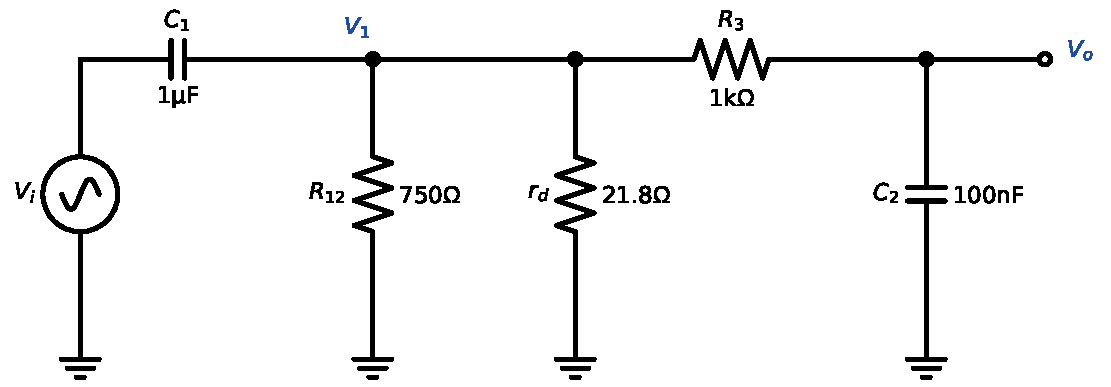
\includegraphics[width=0.95\linewidth,height=5.2cm,keepaspectratio]{p12_ac}\end{center}

\solstep{4}{Transfer function by a chain of dividers}Walk from the input to the output through the named nodes: $V_{i} \to V_{1} \to V_{o}$. The transfer function is the product of the node-to-node ratios (each one is a simple divider, tool T2, or a dependent source, tool T4):
\[
H(s) = \frac{V_o}{V_i} = \frac{V_{1}}{V_{i}}\cdot\frac{V_{o}}{V_{1}}
\]

Impedances seen \emph{looking right} from a node (everything from that node to ground, excluding what is on its left). Compute them from the far right toward the input:
\begin{align*}
Z_{1} &= R_{12} \parallel r_d \parallel \left(R_{3} + \frac{1}{sC_{2}}\right) = \dfrac{20.7\,s + 2.07\times 10^{5}}{s + 9790}
\end{align*}

Now each link. {\small (Algebra tip: to simplify a fraction that contains fractions, multiply its top and bottom by every inner denominator; then divide top and bottom by the leading coefficient of the denominator so that it starts with a plain $s^n$.)}
\begin{align*}
\frac{V_{1}}{V_{i}} &= \frac{Z_{1}}{\frac{1}{sC_{1}} + Z_{1}} = \dfrac{s^{2} + 10000\,s}{s^{2} + 58300\,s + 4.73\times 10^{8}} \\
\frac{V_{o}}{V_{1}} &= \frac{\frac{1}{sC_{2}}}{R_{3} + \frac{1}{sC_{2}}} = \dfrac{10000}{s + 10000}
\end{align*}
Multiply the links and simplify:\[
H(s) = \dfrac{10000\,s}{s^{2} + 58300\,s + 4.73\times 10^{8}}
\]

\solstep{5}{Standard (Bode-ready) form}Find the roots. Every root $s=-p$ of the denominator is a \emph{pole}, every root $s=-z$ of the numerator is a \emph{zero}; $|p|$ and $|z|$ are the corner frequencies (rad/s).
\begin{itemize}[leftmargin=*,itemsep=2pt]
\item Numerator: it has the factor $s$ $\Rightarrow$ 1 zero at $s=0$.
\item Denominator: $s^{2} + 58300\,s + 4.73\times 10^{8}$; quadratic formula:\[
s = \frac{-58300 \pm \sqrt{(58300)^2 - 4(4.73\times 10^{8})}}{2} = \frac{-58300 \pm 38800}{2} \Rightarrow s = -9740,\ -48500
\]

\end{itemize}

Factored form (leading coefficient in front):
\[
H(s) = 10000\,\dfrac{s}{(s+9740)(s+48500)}
\]

Bode-ready form: rewrite every $(s+p) = p\left(1+\frac{s}{p}\right)$ and $(s+z) = z\left(1+\frac{s}{z}\right)$, and collect all constants into $K$. Each $s$ in the numerator is paired with one of the \emph{lowest} poles as $\frac{s}{s+p}$ (that factor is $\approx 1$ above $p$). Then every factor except $K$ is $\approx 1$ inside the pass-band:
\[
H(s) = 0.206\,\dfrac{s}{s+2\pi\cdot 1.55\mathrm{k}}\,\dfrac{1}{1+\dfrac{s}{2\pi\cdot 7.72\mathrm{k}}},\qquad K = 0.206
\]

\begin{center}\renewcommand{\arraystretch}{1.35}
\begin{tabular}{cccc}
\toprule
type & $\omega_c$ (rad/s) & $f_c=\omega_c/2\pi$ & slope change \\
\midrule
pole & $9740$ & 1.55 kHz & $-20$ dB/dec \\
pole & $48500$ & 7.72 kHz & $-20$ dB/dec \\
\bottomrule
\end{tabular}\end{center}

\solstep{6}{Magnitude Bode plot}Below every corner $|H(s)|\approx 2.12\times 10^{-5}\,s$, so the plot starts with a slope of $+20$\,dB/dec. Then, moving right, each pole bends the line down by 20\,dB/dec and each zero bends it up by 20\,dB/dec (tool T6):
\begin{center}\renewcommand{\arraystretch}{1.35}
\begin{tabular}{lcl}
\toprule
frequency range & slope & asymptote level \\
\midrule
$f<$ 1.55 kHz & $+20$ dB/dec & -13.7 dB at end \\
1.55 kHz -- 7.72 kHz & $0$ dB/dec (flat) & -13.7 dB at start, -13.7 dB at end \\
$f>$ 7.72 kHz & $-20$ dB/dec & -13.7 dB at start \\
\bottomrule
\end{tabular}\end{center}

The flat (pass-band) level is $20\log_{10}|K| = 20\log_{10}0.206 = -13.7$\,dB.
\begin{center}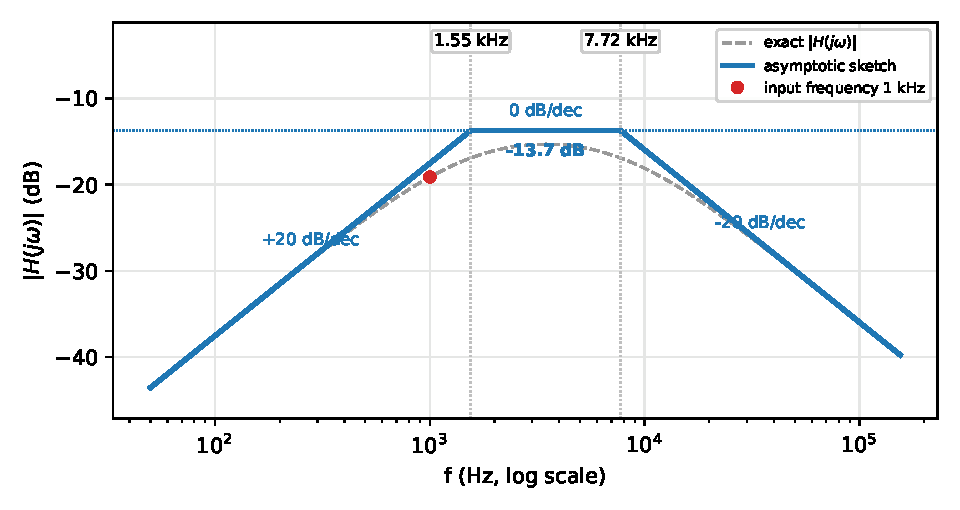
\includegraphics[width=0.78\linewidth,height=6.5cm,keepaspectratio]{p12_bode}\end{center}

{\small Blue: the straight-line sketch you are expected to draw. Dashed grey: the exact curve (about 3\,dB below the corner of an isolated pole). Red dot: the input frequency of Step 7.}
\solstep{7}{Total output (DC + AC)}The input is $V_i(t) = 0.002\sin\left(2\pi\cdot 1000\,t\right)$, so $\omega_{in} = 2\pi\cdot 1000 = 6280$\,rad/s. Put $s=j\omega_{in}$ in each factor (tool T5): magnitudes multiply, angles add.
{\small Rules: $\left|\frac{s}{s+p}\right| = \frac{\omega}{\sqrt{\omega^2+p^2}}$, $\angle = \frac{\pi}{2}-\tan^{-1}\frac{\omega}{p}$;\quad $\left|\frac{1}{1+s/p}\right| = \frac{1}{\sqrt{1+(\omega/p)^2}}$, $\angle = -\tan^{-1}\frac{\omega}{p}$;\quad $\left|1+\frac{s}{z}\right| = \sqrt{1+(\omega/z)^2}$, $\angle = \tan^{-1}\frac{\omega}{z}$;\quad a negative $K$ adds $-\pi$.}
\begin{center}\renewcommand{\arraystretch}{1.35}
\begin{tabular}{ccc}
\toprule
factor & magnitude & angle (rad) \\
\midrule
$0.206$ & $0.2061$ & $0$ \\
$\rule[-1.1em]{0pt}{2.8em}\dfrac{s}{s+2\pi\cdot 1.55\mathrm{k}}$ & $0.5421$ & $0.998$ \\
$\rule[-1.7em]{0pt}{4em}\dfrac{1}{1+\dfrac{s}{2\pi\cdot 7.72\mathrm{k}}}$ & $0.9917$ & $-0.129$ \\
\textbf{total} & $\mathbf{0.1108}$ (product) & $\mathbf{0.869}$ (sum) \\
\bottomrule
\end{tabular}\end{center}

\begin{align*}
|H(j\omega_{in})| &= 0.111, \qquad \angle H(j\omega_{in}) = 0.869\ \mathrm{rad} \\
v_{o,ac}(t) &= 0.111\times 0.002\,\sin\left(2\pi\cdot 1000\,t + 0.869\right) = 2.22\times 10^{-4}\,\sin\left(2\pi\cdot 1000\,t + 0.869\right)
\end{align*}

Add the DC part from Step 2 (superposition):
\[
\boxed{V_o(t) = 0.7 + 2.22\times 10^{-4}\,\sin\left(2\pi\cdot 1000\,t + 0.869\right)\ \mathrm{V}}
\]
 Check the small-signal assumption: the AC voltage across the diode has amplitude about $262\,\mu \mathrm{V}$, well below $nV_T = 45\,\mathrm{m}\mathrm{V}$ \checkmark.
\begin{ansbox}
$H(s) = 0.206\,\dfrac{s}{s+2\pi\cdot 1.55\mathrm{k}}\,\dfrac{1}{1+\dfrac{s}{2\pi\cdot 7.72\mathrm{k}}}$\quad (corners: 1.55 kHz, 7.72 kHz)\\[4pt]
$V_o(t) = 0.7 + 2.22\times 10^{-4}\,\sin\left(2\pi\cdot 1000\,t + 0.869\right)\ \mathrm{V}$
\end{ansbox}

\newpage
\subsection*{Solution 3D.13 \hfill Hard}
\begin{center}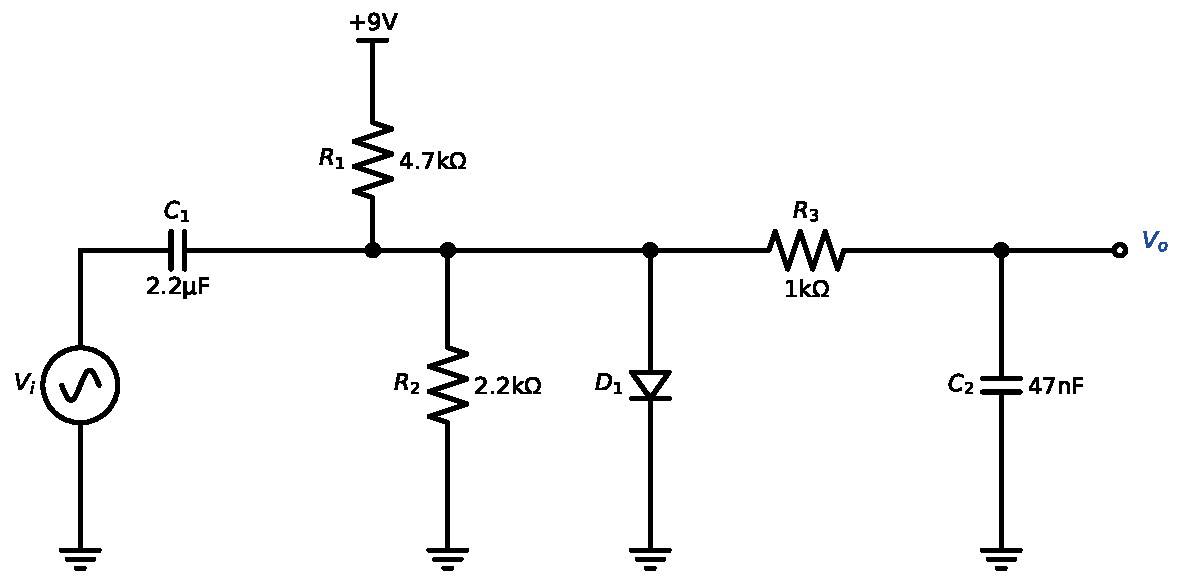
\includegraphics[width=0.9\linewidth,height=5cm,keepaspectratio]{p13_circuit}\end{center}
\solstep{1}{DC operating point}DC rules (tool T3): $v_i = 0$ and every capacitor is open ($C_{1}, C_{2}$). With the exponential model the diode voltage is unknown, so first reduce the rest of the circuit to what the diode sees: a Thevenin source. Remove the diode and solve the circuit (Lecture 2 KCL): the open-circuit voltage across it is $V_{th} = 2.87\,\mathrm{V}$. Short the diode instead: the current is $I_{sc} = 1.91\,\mathrm{m}\mathrm{A}$. So $R_{th} = \frac{V_{th}}{I_{sc}} = 1.5\,\mathrm{k}\Omega$.

Two equations, two unknowns: the circuit gives $I_D = \frac{V_{th}-V_D}{R_{th}}$ and the diode gives $V_D = nV_T\ln\frac{I_D}{I_S}$ (tool T1, $n=1$, $V_T = 25$\,mV, $I_S = 1\,\mathrm{p}\mathrm{A}$). Solve by iteration: guess $V_D = 0.7$\,V, compute $I_D$, update $V_D$, repeat until nothing changes:\begin{center}\renewcommand{\arraystretch}{1.35}
\begin{tabular}{cccc}
\toprule
step & $V_D$ used (V) & circuit $\Rightarrow I_D$ & diode $\Rightarrow$ new $V_D$ (V) \\
\midrule
1 & $0.7$ & $I_D = \frac{2.87 - 0.7}{1499} = 1.45\,\mathrm{m}\mathrm{A}$ & $0.5273$ \\
2 & $0.5273$ & $I_D = \frac{2.87 - 0.5273}{1499} = 1.56\,\mathrm{m}\mathrm{A}$ & $0.5292$ \\
3 & $0.5292$ & $I_D = \frac{2.87 - 0.5292}{1499} = 1.56\,\mathrm{m}\mathrm{A}$ & $0.5292$ \\
4 & $0.5292$ & $I_D = \frac{2.87 - 0.5292}{1499} = 1.56\,\mathrm{m}\mathrm{A}$ & $0.5292$ \\
5 & $0.5292$ & $I_D = \frac{2.87 - 0.5292}{1499} = 1.56\,\mathrm{m}\mathrm{A}$ & $0.5292$ \\
\bottomrule
\end{tabular}\end{center}
Converged: $V_D = 0.5292$\,V, $I_D = 1.56\,\mathrm{m}\mathrm{A}$. With this $V_D$ the rest of the DC circuit gives $V_{o,dc} = 529\,\mathrm{m}\mathrm{V}$.\[
\boxed{V_{o,dc} = 529\,\mathrm{m}\mathrm{V}}
\]

\solstep{2}{Small-signal resistance}$r_{d} = \frac{nV_T}{I_D} = \frac{1\times 25\,\mathrm{mV}}{1.56\,\mathrm{m}\mathrm{A}} = 16\,\Omega$ (tool T3). For the AC analysis the diode is just this resistor.
\solstep{3}{AC circuit}Set every DC supply to zero: each supply rail becomes AC ground. Replace every capacitor by $\frac{1}{sC}$ and every inductor by $sL$.
\begin{itemize}[leftmargin=*,itemsep=2pt]
\item $R_{1}$, $R_{2}$ both go from the same node to (AC) ground, so they are in parallel: $R_{12} = R_{1} \parallel R_{2} = 4.7\,\mathrm{k} \parallel 2.2\,\mathrm{k} = 1.5\,\mathrm{k}\Omega$.
\end{itemize}

AC equivalent circuit (nodes named for the next step):
\begin{center}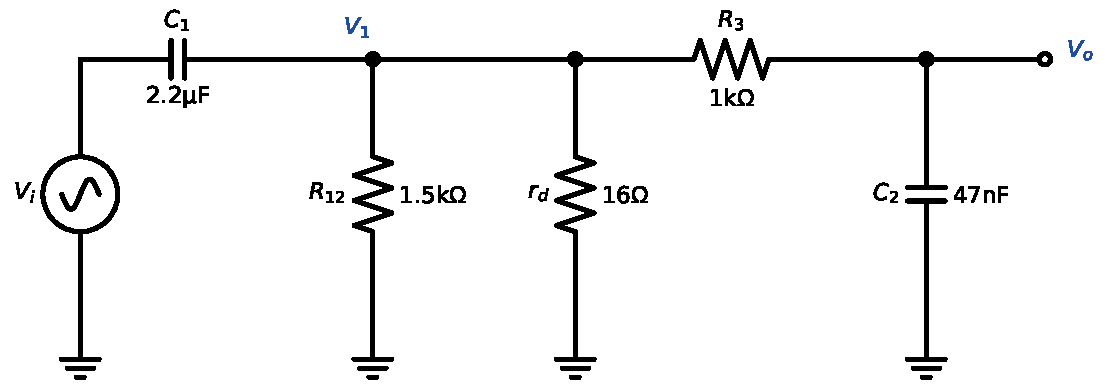
\includegraphics[width=0.95\linewidth,height=5.2cm,keepaspectratio]{p13_ac}\end{center}

\solstep{4}{Transfer function by a chain of dividers}Walk from the input to the output through the named nodes: $V_{i} \to V_{1} \to V_{o}$. The transfer function is the product of the node-to-node ratios (each one is a simple divider, tool T2, or a dependent source, tool T4):
\[
H(s) = \frac{V_o}{V_i} = \frac{V_{1}}{V_{i}}\cdot\frac{V_{o}}{V_{1}}
\]

Impedances seen \emph{looking right} from a node (everything from that node to ground, excluding what is on its left). Compute them from the far right toward the input:
\begin{align*}
Z_{1} &= R_{12} \parallel r_d \parallel \left(R_{3} + \frac{1}{sC_{2}}\right) = \dfrac{15.6\,s + 3.32\times 10^{5}}{s + 20900}
\end{align*}

Now each link. {\small (Algebra tip: to simplify a fraction that contains fractions, multiply its top and bottom by every inner denominator; then divide top and bottom by the leading coefficient of the denominator so that it starts with a plain $s^n$.)}
\begin{align*}
\frac{V_{1}}{V_{i}} &= \frac{Z_{1}}{\frac{1}{sC_{1}} + Z_{1}} = \dfrac{s^{2} + 21300\,s}{s^{2} + 50400\,s + 6.11\times 10^{8}} \\
\frac{V_{o}}{V_{1}} &= \frac{\frac{1}{sC_{2}}}{R_{3} + \frac{1}{sC_{2}}} = \dfrac{21300}{s + 21300}
\end{align*}
Multiply the links and simplify:\[
H(s) = \dfrac{21300\,s}{s^{2} + 50400\,s + 6.11\times 10^{8}}
\]

\solstep{5}{Standard (Bode-ready) form}Find the roots. Every root $s=-p$ of the denominator is a \emph{pole}, every root $s=-z$ of the numerator is a \emph{zero}; $|p|$ and $|z|$ are the corner frequencies (rad/s).
\begin{itemize}[leftmargin=*,itemsep=2pt]
\item Numerator: it has the factor $s$ $\Rightarrow$ 1 zero at $s=0$.
\item Denominator: $s^{2} + 50400\,s + 6.11\times 10^{8}$; quadratic formula:\[
s = \frac{-50400 \pm \sqrt{(50400)^2 - 4(6.11\times 10^{8})}}{2} = \frac{-50400 \pm 10000}{2} \Rightarrow s = -20200,\ -30200
\]

\end{itemize}

Factored form (leading coefficient in front):
\[
H(s) = 21300\,\dfrac{s}{(s+20200)(s+30200)}
\]

Bode-ready form: rewrite every $(s+p) = p\left(1+\frac{s}{p}\right)$ and $(s+z) = z\left(1+\frac{s}{z}\right)$, and collect all constants into $K$. Each $s$ in the numerator is paired with one of the \emph{lowest} poles as $\frac{s}{s+p}$ (that factor is $\approx 1$ above $p$). Then every factor except $K$ is $\approx 1$ inside the pass-band:
\[
H(s) = 0.704\,\dfrac{s}{s+2\pi\cdot 3.21\mathrm{k}}\,\dfrac{1}{1+\dfrac{s}{2\pi\cdot 4.81\mathrm{k}}},\qquad K = 0.704
\]

\begin{center}\renewcommand{\arraystretch}{1.35}
\begin{tabular}{cccc}
\toprule
type & $\omega_c$ (rad/s) & $f_c=\omega_c/2\pi$ & slope change \\
\midrule
pole & $20200$ & 3.21 kHz & $-20$ dB/dec \\
pole & $30200$ & 4.81 kHz & $-20$ dB/dec \\
\bottomrule
\end{tabular}\end{center}

\solstep{6}{Magnitude Bode plot}Below every corner $|H(s)|\approx 3.48\times 10^{-5}\,s$, so the plot starts with a slope of $+20$\,dB/dec. Then, moving right, each pole bends the line down by 20\,dB/dec and each zero bends it up by 20\,dB/dec (tool T6):
\begin{center}\renewcommand{\arraystretch}{1.35}
\begin{tabular}{lcl}
\toprule
frequency range & slope & asymptote level \\
\midrule
$f<$ 3.21 kHz & $+20$ dB/dec & -3.05 dB at end \\
3.21 kHz -- 4.81 kHz & $0$ dB/dec (flat) & -3.05 dB at start, -3.05 dB at end \\
$f>$ 4.81 kHz & $-20$ dB/dec & -3.05 dB at start \\
\bottomrule
\end{tabular}\end{center}

The flat (pass-band) level is $20\log_{10}|K| = 20\log_{10}0.704 = -3.05$\,dB.
\begin{center}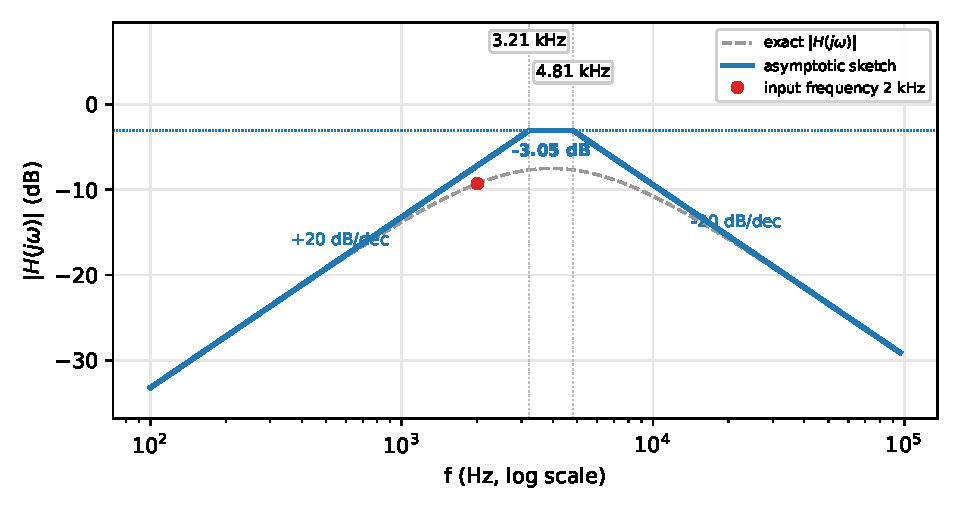
\includegraphics[width=0.78\linewidth,height=6.5cm,keepaspectratio]{p13_bode}\end{center}

{\small Blue: the straight-line sketch you are expected to draw. Dashed grey: the exact curve (about 3\,dB below the corner of an isolated pole). Red dot: the input frequency of Step 7.}
\solstep{7}{Total output (DC + AC)}The input is $V_i(t) = 0.003\sin\left(2\pi\cdot 2000\,t\right)$, so $\omega_{in} = 2\pi\cdot 2000 = 12600$\,rad/s. Put $s=j\omega_{in}$ in each factor (tool T5): magnitudes multiply, angles add.
{\small Rules: $\left|\frac{s}{s+p}\right| = \frac{\omega}{\sqrt{\omega^2+p^2}}$, $\angle = \frac{\pi}{2}-\tan^{-1}\frac{\omega}{p}$;\quad $\left|\frac{1}{1+s/p}\right| = \frac{1}{\sqrt{1+(\omega/p)^2}}$, $\angle = -\tan^{-1}\frac{\omega}{p}$;\quad $\left|1+\frac{s}{z}\right| = \sqrt{1+(\omega/z)^2}$, $\angle = \tan^{-1}\frac{\omega}{z}$;\quad a negative $K$ adds $-\pi$.}
\begin{center}\renewcommand{\arraystretch}{1.35}
\begin{tabular}{ccc}
\toprule
factor & magnitude & angle (rad) \\
\midrule
$0.704$ & $0.7038$ & $0$ \\
$\rule[-1.1em]{0pt}{2.8em}\dfrac{s}{s+2\pi\cdot 3.21\mathrm{k}}$ & $0.5283$ & $1.01$ \\
$\rule[-1.7em]{0pt}{4em}\dfrac{1}{1+\dfrac{s}{2\pi\cdot 4.81\mathrm{k}}}$ & $0.9234$ & $-0.394$ \\
\textbf{total} & $\mathbf{0.3433}$ (product) & $\mathbf{0.62}$ (sum) \\
\bottomrule
\end{tabular}\end{center}

\begin{align*}
|H(j\omega_{in})| &= 0.343, \qquad \angle H(j\omega_{in}) = 0.62\ \mathrm{rad} \\
v_{o,ac}(t) &= 0.343\times 0.003\,\sin\left(2\pi\cdot 2000\,t + 0.62\right) = 0.00103\,\sin\left(2\pi\cdot 2000\,t + 0.62\right)
\end{align*}

Add the DC part from Step 2 (superposition):
\[
\boxed{V_o(t) = 0.529 + 0.00103\,\sin\left(2\pi\cdot 2000\,t + 0.62\right)\ \mathrm{V}}
\]
 Check the small-signal assumption: the AC voltage across the diode has amplitude about $1.2\,\mathrm{m}\mathrm{V}$, well below $nV_T = 25\,\mathrm{m}\mathrm{V}$ \checkmark.
\begin{ansbox}
$H(s) = 0.704\,\dfrac{s}{s+2\pi\cdot 3.21\mathrm{k}}\,\dfrac{1}{1+\dfrac{s}{2\pi\cdot 4.81\mathrm{k}}}$\quad (corners: 3.21 kHz, 4.81 kHz)\\[4pt]
$V_o(t) = 0.529 + 0.00103\,\sin\left(2\pi\cdot 2000\,t + 0.62\right)\ \mathrm{V}$
\end{ansbox}

\newpage
\subsection*{Solution 3D.14 \hfill Hard}
\begin{center}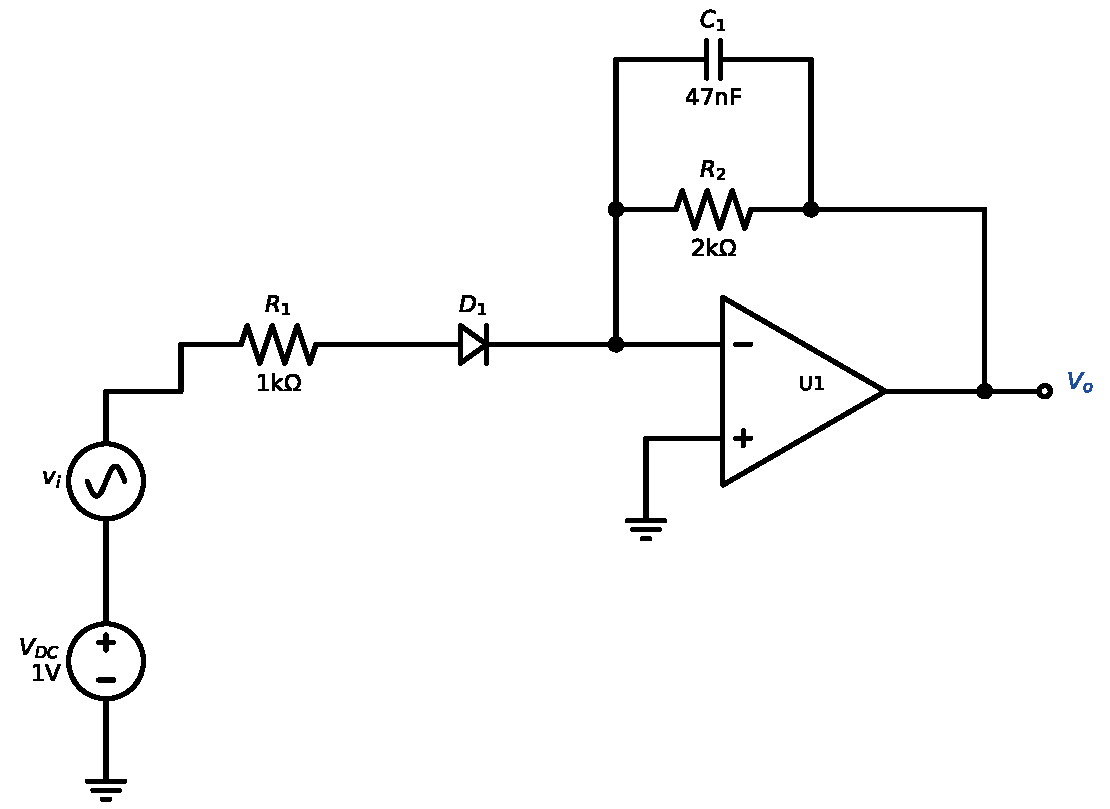
\includegraphics[width=0.9\linewidth,height=5cm,keepaspectratio]{p14_circuit}\end{center}
\solstep{1}{DC operating point}DC rules (tool T3): $v_i = 0$, so the input is just $V_{DC} = 1\,\mathrm{V}$; capacitors are open. The op-amp has negative feedback, so $V_- = V_+ = 0$ (virtual ground) and no current enters its inputs. The diode and $R_{1}$ connect $V_{DC}$ to the virtual ground: the diode sees $V_{th} = V_{DC}$ through $R_{th} = R_{1} = 1\,\mathrm{k}\Omega$.

Two equations, two unknowns: the circuit gives $I_D = \frac{V_{th}-V_D}{R_{th}}$ and the diode gives $V_D = nV_T\ln\frac{I_D}{I_S}$ (tool T1, $n=1.8$, $V_T = 25$\,mV, $I_S = 2.6\,\mathrm{n}\mathrm{A}$). Solve by iteration: guess $V_D = 0.7$\,V, compute $I_D$, update $V_D$, repeat until nothing changes:\begin{center}\renewcommand{\arraystretch}{1.35}
\begin{tabular}{cccc}
\toprule
step & $V_D$ used (V) & circuit $\Rightarrow I_D$ & diode $\Rightarrow$ new $V_D$ (V) \\
\midrule
1 & $0.7$ & $I_D = \frac{1 - 0.7}{1000} = 300\,\mu \mathrm{A}$ & $0.5245$ \\
2 & $0.5245$ & $I_D = \frac{1 - 0.5245}{1000} = 475\,\mu \mathrm{A}$ & $0.5452$ \\
3 & $0.5452$ & $I_D = \frac{1 - 0.5452}{1000} = 455\,\mu \mathrm{A}$ & $0.5432$ \\
4 & $0.5432$ & $I_D = \frac{1 - 0.5432}{1000} = 457\,\mu \mathrm{A}$ & $0.5434$ \\
5 & $0.5434$ & $I_D = \frac{1 - 0.5434}{1000} = 457\,\mu \mathrm{A}$ & $0.5434$ \\
\bottomrule
\end{tabular}\end{center}
Converged: $I_D = 457\,\mu \mathrm{A}$. All of $I_D$ continues through the feedback resistor $R_{2}$ (the capacitor is open), so\[
V_{o,dc} = 0 - R_{2}I_D = -2000\times4.566\times 10^{-4} = -913\,\mathrm{m}\mathrm{V}
\]
\[
\boxed{V_{o,dc} = -913\,\mathrm{m}\mathrm{V}}
\]

\solstep{2}{Small-signal resistance}$r_d = \frac{nV_T}{I_D} = \frac{1.8\times 25\,\mathrm{mV}}{457\,\mu \mathrm{A}} = 98.6\,\Omega$ (tool T3). For the AC analysis the diode is just this resistor, and $V_{DC}$ is replaced by a short (AC ground).
\solstep{3}{AC circuit}\begin{center}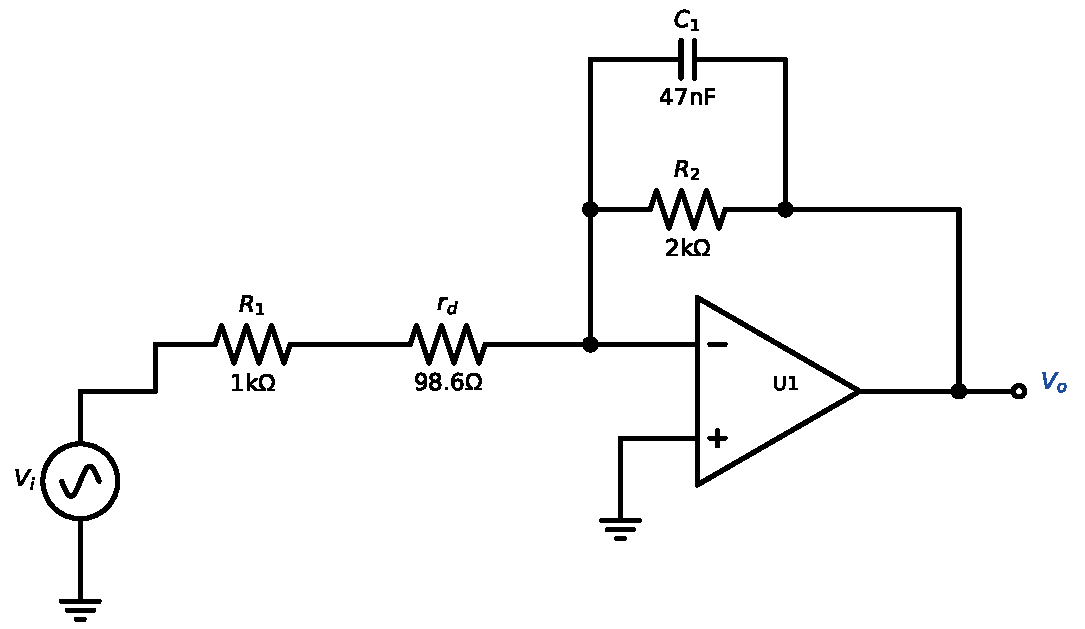
\includegraphics[width=0.9\linewidth,height=5cm,keepaspectratio]{p14_ac}\end{center}

\solstep{4}{Transfer function}\textbf{Block 1 (U1).} Inverting block: the $+$ input is grounded, so $V_- = V_+ = 0$ (virtual ground). The current $\frac{V_{i} - 0}{Z_{in1}}$ through $Z_{in1}$ cannot enter the op-amp, so all of it flows through $Z_{f1}$: $V_{o} = 0 - Z_{f1}\cdot\frac{V_{i}}{Z_{in1}}$.\begin{align*}
Z_{in1} &= R_{1} + r_d = 1100 \\
Z_{f1} &= R_{2} \parallel \frac{1}{sC_{1}} = \dfrac{2.13\times 10^{7}}{s + 10600}
\end{align*}
\[
\frac{V_{o}}{V_{i}} = -\frac{Z_{f1}}{Z_{in1}} = \dfrac{-19400}{s + 10600}
\]
So:\[
H(s) = \dfrac{-19400}{s + 10600}
\]

\solstep{5}{Standard (Bode-ready) form}Find the roots. Every root $s=-p$ of the denominator is a \emph{pole}, every root $s=-z$ of the numerator is a \emph{zero}; $|p|$ and $|z|$ are the corner frequencies (rad/s).
\begin{itemize}[leftmargin=*,itemsep=2pt]
\item Denominator: $s + 10600$; $s + 10600 = 0 \Rightarrow s = -10600$.
\end{itemize}

Factored form (leading coefficient in front):
\[
H(s) = -19400\,\dfrac{1}{(s+10600)}
\]

Bode-ready form: rewrite every $(s+p) = p\left(1+\frac{s}{p}\right)$ and $(s+z) = z\left(1+\frac{s}{z}\right)$, and collect all constants into $K$. Then every factor except $K$ is $\approx 1$ inside the pass-band:
\[
H(s) = -1.82\,\dfrac{1}{1+\dfrac{s}{2\pi\cdot 1.69\mathrm{k}}},\qquad K = -1.82
\]

\begin{center}\renewcommand{\arraystretch}{1.35}
\begin{tabular}{cccc}
\toprule
type & $\omega_c$ (rad/s) & $f_c=\omega_c/2\pi$ & slope change \\
\midrule
pole & $10600$ & 1.69 kHz & $-20$ dB/dec \\
\bottomrule
\end{tabular}\end{center}

\solstep{6}{Magnitude Bode plot}Below every corner, all factors are $\approx$ constant: $|H| \approx 1.82$ $= 5.2$\,dB (flat, 0 dB/dec). Then, moving right, each pole bends the line down by 20\,dB/dec and each zero bends it up by 20\,dB/dec (tool T6):
\begin{center}\renewcommand{\arraystretch}{1.35}
\begin{tabular}{lcl}
\toprule
frequency range & slope & asymptote level \\
\midrule
$f<$ 1.69 kHz & $0$ dB/dec (flat) & 5.2 dB at end \\
$f>$ 1.69 kHz & $-20$ dB/dec & 5.2 dB at start \\
\bottomrule
\end{tabular}\end{center}

The flat (pass-band) level is $20\log_{10}|K| = 20\log_{10}1.82 = 5.2$\,dB.
\begin{center}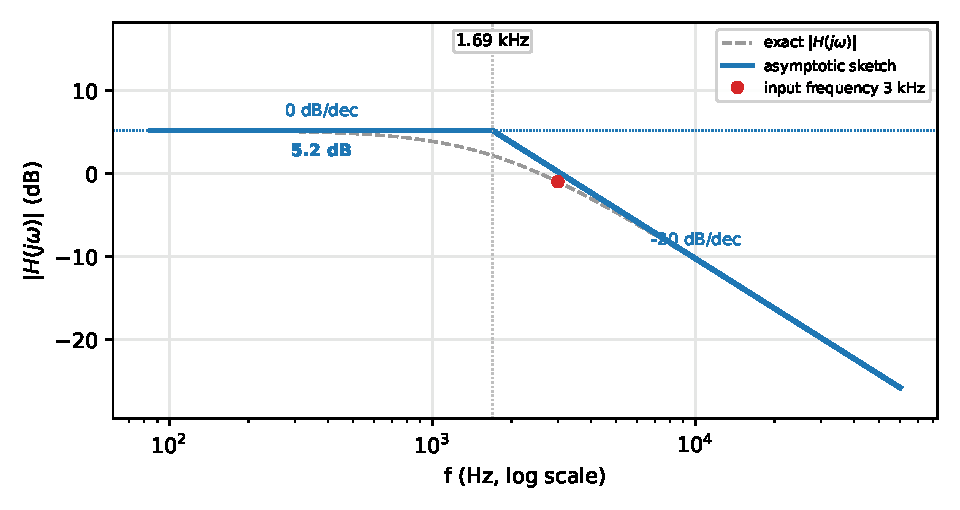
\includegraphics[width=0.78\linewidth,height=6.5cm,keepaspectratio]{p14_bode}\end{center}

{\small Blue: the straight-line sketch you are expected to draw. Dashed grey: the exact curve (about 3\,dB below the corner of an isolated pole). Red dot: the input frequency of Step 7.}
\solstep{7}{Total output (DC + AC)}The input is $V_i(t) = 0.01\sin\left(2\pi\cdot 3000\,t+\frac{\pi}{4}\right)$, so $\omega_{in} = 2\pi\cdot 3000 = 18800$\,rad/s. Put $s=j\omega_{in}$ in each factor (tool T5): magnitudes multiply, angles add.
{\small Rules: $\left|\frac{s}{s+p}\right| = \frac{\omega}{\sqrt{\omega^2+p^2}}$, $\angle = \frac{\pi}{2}-\tan^{-1}\frac{\omega}{p}$;\quad $\left|\frac{1}{1+s/p}\right| = \frac{1}{\sqrt{1+(\omega/p)^2}}$, $\angle = -\tan^{-1}\frac{\omega}{p}$;\quad $\left|1+\frac{s}{z}\right| = \sqrt{1+(\omega/z)^2}$, $\angle = \tan^{-1}\frac{\omega}{z}$;\quad a negative $K$ adds $-\pi$.}
\begin{center}\renewcommand{\arraystretch}{1.35}
\begin{tabular}{ccc}
\toprule
factor & magnitude & angle (rad) \\
\midrule
$-1.82$ & $1.821$ & $-3.14$ \\
$\rule[-1.7em]{0pt}{4em}\dfrac{1}{1+\dfrac{s}{2\pi\cdot 1.69\mathrm{k}}}$ & $0.4915$ & $-1.06$ \\
\textbf{total} & $\mathbf{0.8948}$ (product) & $\mathbf{-4.2}$ (sum) \\
\bottomrule
\end{tabular}\end{center}

\begin{align*}
|H(j\omega_{in})| &= 0.895, \qquad \angle H(j\omega_{in}) = -4.2\ \mathrm{rad} \\
v_{o,ac}(t) &= 0.895\times 0.01\,\sin\left(2\pi\cdot 3000\,t - 3.41\right) = 0.00895\,\sin\left(2\pi\cdot 3000\,t - 3.41\right)
\end{align*}

(phase: $\theta + \angle H = \frac{\pi}{4} + (-4.2) = -3.41$\,rad.)
Add the DC part from Step 2 (superposition):
\[
\boxed{V_o(t) = -0.913 + 0.00895\,\sin\left(2\pi\cdot 3000\,t - 3.41\right)\ \mathrm{V}}
\]
 Check the small-signal assumption: the AC voltage across the diode has amplitude about $897\,\mu \mathrm{V}$, well below $nV_T = 45\,\mathrm{m}\mathrm{V}$ \checkmark.
\begin{ansbox}
$H(s) = -1.82\,\dfrac{1}{1+\dfrac{s}{2\pi\cdot 1.69\mathrm{k}}}$\quad (corners: 1.69 kHz)\\[4pt]
$V_o(t) = -0.913 + 0.00895\,\sin\left(2\pi\cdot 3000\,t - 3.41\right)\ \mathrm{V}$
\end{ansbox}

\newpage
\subsection*{Solution 3D.15 \hfill Hard}
\begin{center}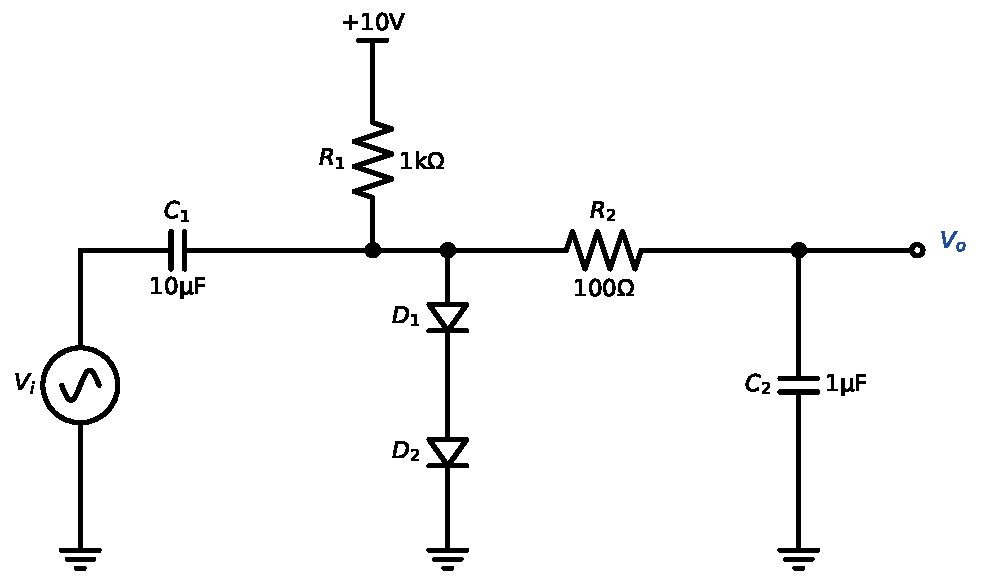
\includegraphics[width=0.9\linewidth,height=5cm,keepaspectratio]{p15_circuit}\end{center}
\solstep{1}{DC operating point}DC rules (tool T3): $v_i = 0$ and every capacitor is open ($C_{1}, C_{2}$). Assume both diodes are ON ($0.7$\,V each) and solve the DC circuit:

Replace $D_{1}$ ON: a $0.7$\,V source ($V_{1} - V_{a} = 0.7$) carrying an unknown current $I_{D_{1}}$ from anode to cathode; $D_{2}$ ON: a $0.7$\,V source ($V_{a} - 0 = 0.7$) carrying an unknown current $I_{D_{2}}$ from anode to cathode.

Equations (KCL at every node that is not an op-amp output, plus the diode voltages):\begin{align*}
&\text{KCL at }V_{1}: && \frac{V_{1} - 10}{R_{1}} + \frac{V_{1} - V_{o}}{R_{2}} + I_{D_{1}} = 0 \\
&\text{KCL at }V_{a}: && - I_{D_{1}} + I_{D_{2}} = 0 \\
&\text{KCL at }V_{o}: && \frac{V_{o} - V_{1}}{R_{2}} = 0 \\
&\text{D1 ON}: && V_{1} - V_{a} = 0.7 \\
&\text{D2 ON}: && V_{a} - 0 = 0.7
\end{align*}


Solving these linear equations (substitute one into the other, as in Lecture 2) gives, with $V_i$ kept as a symbol:\begin{align*}
V_{o} &= 1.4 \\
I_{D_{1}} &= 8.6\ \mathrm{mA} \\
I_{D_{2}} &= 8.6\ \mathrm{mA}
\end{align*}


 $I_{D_{1}} = 8.6\,\mathrm{m}\mathrm{A} > 0$, $I_{D_{2}} = 8.6\,\mathrm{m}\mathrm{A} > 0$ \checkmark, so the assumption holds.\[
\boxed{V_{o,dc} = 1.4\,\mathrm{V}}
\]

\solstep{2}{Small-signal resistance}$r_{d} = \frac{nV_T}{I_D} = \frac{1.8\times 25\,\mathrm{mV}}{8.6\,\mathrm{m}\mathrm{A}} = 5.23\,\Omega$ $r_{d} = \frac{nV_T}{I_D} = \frac{1.8\times 25\,\mathrm{mV}}{8.6\,\mathrm{m}\mathrm{A}} = 5.23\,\Omega$ (tool T3). For the AC analysis the diode is just this resistor.
\solstep{3}{AC circuit}Set every DC supply to zero: each supply rail becomes AC ground. Replace every capacitor by $\frac{1}{sC}$ and every inductor by $sL$.
AC equivalent circuit (nodes named for the next step):
\begin{center}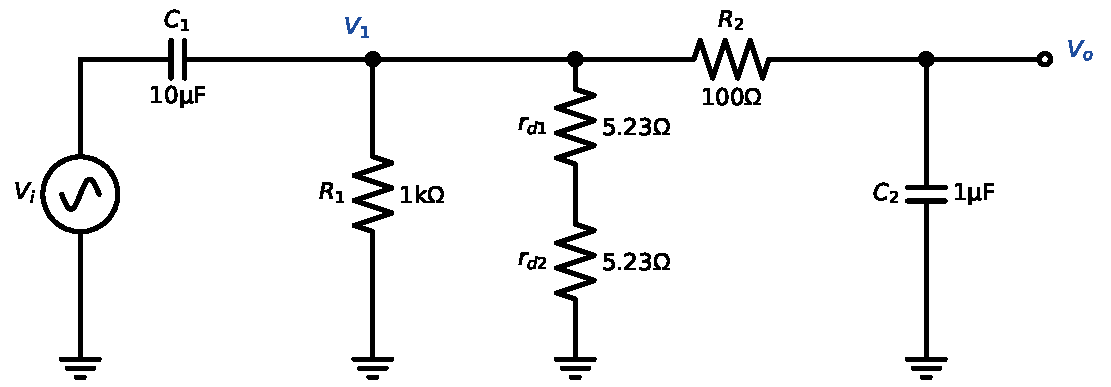
\includegraphics[width=0.95\linewidth,height=5.2cm,keepaspectratio]{p15_ac}\end{center}

\solstep{4}{Transfer function by a chain of dividers}Walk from the input to the output through the named nodes: $V_{i} \to V_{1} \to V_{o}$. The transfer function is the product of the node-to-node ratios (each one is a simple divider, tool T2, or a dependent source, tool T4):
\[
H(s) = \frac{V_o}{V_i} = \frac{V_{1}}{V_{i}}\cdot\frac{V_{o}}{V_{1}}
\]

Impedances seen \emph{looking right} from a node (everything from that node to ground, excluding what is on its left). Compute them from the far right toward the input:
\begin{align*}
Z_{1} &= R_{1} \parallel \left(r_{d1} + r_{d2}\right) \parallel \left(R_{2} + \frac{1}{sC_{2}}\right) = \dfrac{9.38\,s + 93800}{s + 9060}
\end{align*}

Now each link. {\small (Algebra tip: to simplify a fraction that contains fractions, multiply its top and bottom by every inner denominator; then divide top and bottom by the leading coefficient of the denominator so that it starts with a plain $s^n$.)}
\begin{align*}
\frac{V_{1}}{V_{i}} &= \frac{Z_{1}}{\frac{1}{sC_{1}} + Z_{1}} = \dfrac{s^{2} + 10000\,s}{s^{2} + 20700\,s + 9.66\times 10^{7}} \\
\frac{V_{o}}{V_{1}} &= \frac{\frac{1}{sC_{2}}}{R_{2} + \frac{1}{sC_{2}}} = \dfrac{10000}{s + 10000}
\end{align*}
Multiply the links and simplify:\[
H(s) = \dfrac{10000\,s}{s^{2} + 20700\,s + 9.66\times 10^{7}}
\]

\solstep{5}{Standard (Bode-ready) form}Find the roots. Every root $s=-p$ of the denominator is a \emph{pole}, every root $s=-z$ of the numerator is a \emph{zero}; $|p|$ and $|z|$ are the corner frequencies (rad/s).
\begin{itemize}[leftmargin=*,itemsep=2pt]
\item Numerator: it has the factor $s$ $\Rightarrow$ 1 zero at $s=0$.
\item Denominator: $s^{2} + 20700\,s + 9.66\times 10^{7}$; quadratic formula:\[
s = \frac{-20700 \pm \sqrt{(20700)^2 - 4(9.66\times 10^{7})}}{2} = \frac{-20700 \pm 6360}{2} \Rightarrow s = -7150,\ -13500
\]

\end{itemize}

Factored form (leading coefficient in front):
\[
H(s) = 10000\,\dfrac{s}{(s+7150)(s+13500)}
\]

Bode-ready form: rewrite every $(s+p) = p\left(1+\frac{s}{p}\right)$ and $(s+z) = z\left(1+\frac{s}{z}\right)$, and collect all constants into $K$. Each $s$ in the numerator is paired with one of the \emph{lowest} poles as $\frac{s}{s+p}$ (that factor is $\approx 1$ above $p$). Then every factor except $K$ is $\approx 1$ inside the pass-band:
\[
H(s) = 0.74\,\dfrac{s}{s+2\pi\cdot 1.14\mathrm{k}}\,\dfrac{1}{1+\dfrac{s}{2\pi\cdot 2.15\mathrm{k}}},\qquad K = 0.74
\]

\begin{center}\renewcommand{\arraystretch}{1.35}
\begin{tabular}{cccc}
\toprule
type & $\omega_c$ (rad/s) & $f_c=\omega_c/2\pi$ & slope change \\
\midrule
pole & $7150$ & 1.14 kHz & $-20$ dB/dec \\
pole & $13500$ & 2.15 kHz & $-20$ dB/dec \\
\bottomrule
\end{tabular}\end{center}

\solstep{6}{Magnitude Bode plot}Below every corner $|H(s)|\approx 1.04\times 10^{-4}\,s$, so the plot starts with a slope of $+20$\,dB/dec. Then, moving right, each pole bends the line down by 20\,dB/dec and each zero bends it up by 20\,dB/dec (tool T6):
\begin{center}\renewcommand{\arraystretch}{1.35}
\begin{tabular}{lcl}
\toprule
frequency range & slope & asymptote level \\
\midrule
$f<$ 1.14 kHz & $+20$ dB/dec & -2.61 dB at end \\
1.14 kHz -- 2.15 kHz & $0$ dB/dec (flat) & -2.61 dB at start, -2.61 dB at end \\
$f>$ 2.15 kHz & $-20$ dB/dec & -2.61 dB at start \\
\bottomrule
\end{tabular}\end{center}

The flat (pass-band) level is $20\log_{10}|K| = 20\log_{10}0.74 = -2.61$\,dB.
\begin{center}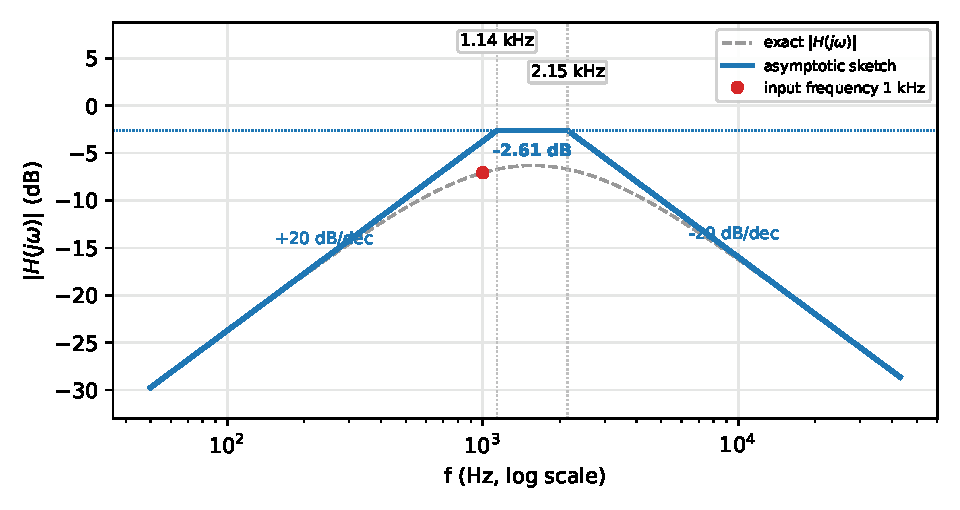
\includegraphics[width=0.78\linewidth,height=6.5cm,keepaspectratio]{p15_bode}\end{center}

{\small Blue: the straight-line sketch you are expected to draw. Dashed grey: the exact curve (about 3\,dB below the corner of an isolated pole). Red dot: the input frequency of Step 7.}
\solstep{7}{Total output (DC + AC)}The input is $V_i(t) = 0.002\sin\left(2\pi\cdot 1000\,t\right)$, so $\omega_{in} = 2\pi\cdot 1000 = 6280$\,rad/s. Put $s=j\omega_{in}$ in each factor (tool T5): magnitudes multiply, angles add.
{\small Rules: $\left|\frac{s}{s+p}\right| = \frac{\omega}{\sqrt{\omega^2+p^2}}$, $\angle = \frac{\pi}{2}-\tan^{-1}\frac{\omega}{p}$;\quad $\left|\frac{1}{1+s/p}\right| = \frac{1}{\sqrt{1+(\omega/p)^2}}$, $\angle = -\tan^{-1}\frac{\omega}{p}$;\quad $\left|1+\frac{s}{z}\right| = \sqrt{1+(\omega/z)^2}$, $\angle = \tan^{-1}\frac{\omega}{z}$;\quad a negative $K$ adds $-\pi$.}
\begin{center}\renewcommand{\arraystretch}{1.35}
\begin{tabular}{ccc}
\toprule
factor & magnitude & angle (rad) \\
\midrule
$0.74$ & $0.7404$ & $0$ \\
$\rule[-1.1em]{0pt}{2.8em}\dfrac{s}{s+2\pi\cdot 1.14\mathrm{k}}$ & $0.6602$ & $0.85$ \\
$\rule[-1.7em]{0pt}{4em}\dfrac{1}{1+\dfrac{s}{2\pi\cdot 2.15\mathrm{k}}}$ & $0.9067$ & $-0.435$ \\
\textbf{total} & $\mathbf{0.4432}$ (product) & $\mathbf{0.414}$ (sum) \\
\bottomrule
\end{tabular}\end{center}

\begin{align*}
|H(j\omega_{in})| &= 0.443, \qquad \angle H(j\omega_{in}) = 0.414\ \mathrm{rad} \\
v_{o,ac}(t) &= 0.443\times 0.002\,\sin\left(2\pi\cdot 1000\,t + 0.414\right) = 8.86\times 10^{-4}\,\sin\left(2\pi\cdot 1000\,t + 0.414\right)
\end{align*}

Add the DC part from Step 2 (superposition):
\[
\boxed{V_o(t) = 1.4 + 8.86\times 10^{-4}\,\sin\left(2\pi\cdot 1000\,t + 0.414\right)\ \mathrm{V}}
\]
 Check the small-signal assumption: the AC voltage across the diode has amplitude about $523\,\mu \mathrm{V}$, well below $nV_T = 45\,\mathrm{m}\mathrm{V}$ \checkmark.
\begin{ansbox}
$H(s) = 0.74\,\dfrac{s}{s+2\pi\cdot 1.14\mathrm{k}}\,\dfrac{1}{1+\dfrac{s}{2\pi\cdot 2.15\mathrm{k}}}$\quad (corners: 1.14 kHz, 2.15 kHz)\\[4pt]
$V_o(t) = 1.4 + 8.86\times 10^{-4}\,\sin\left(2\pi\cdot 1000\,t + 0.414\right)\ \mathrm{V}$
\end{ansbox}

\newpage
\subsection*{Solution 3D.16 \hfill Hard}
\begin{center}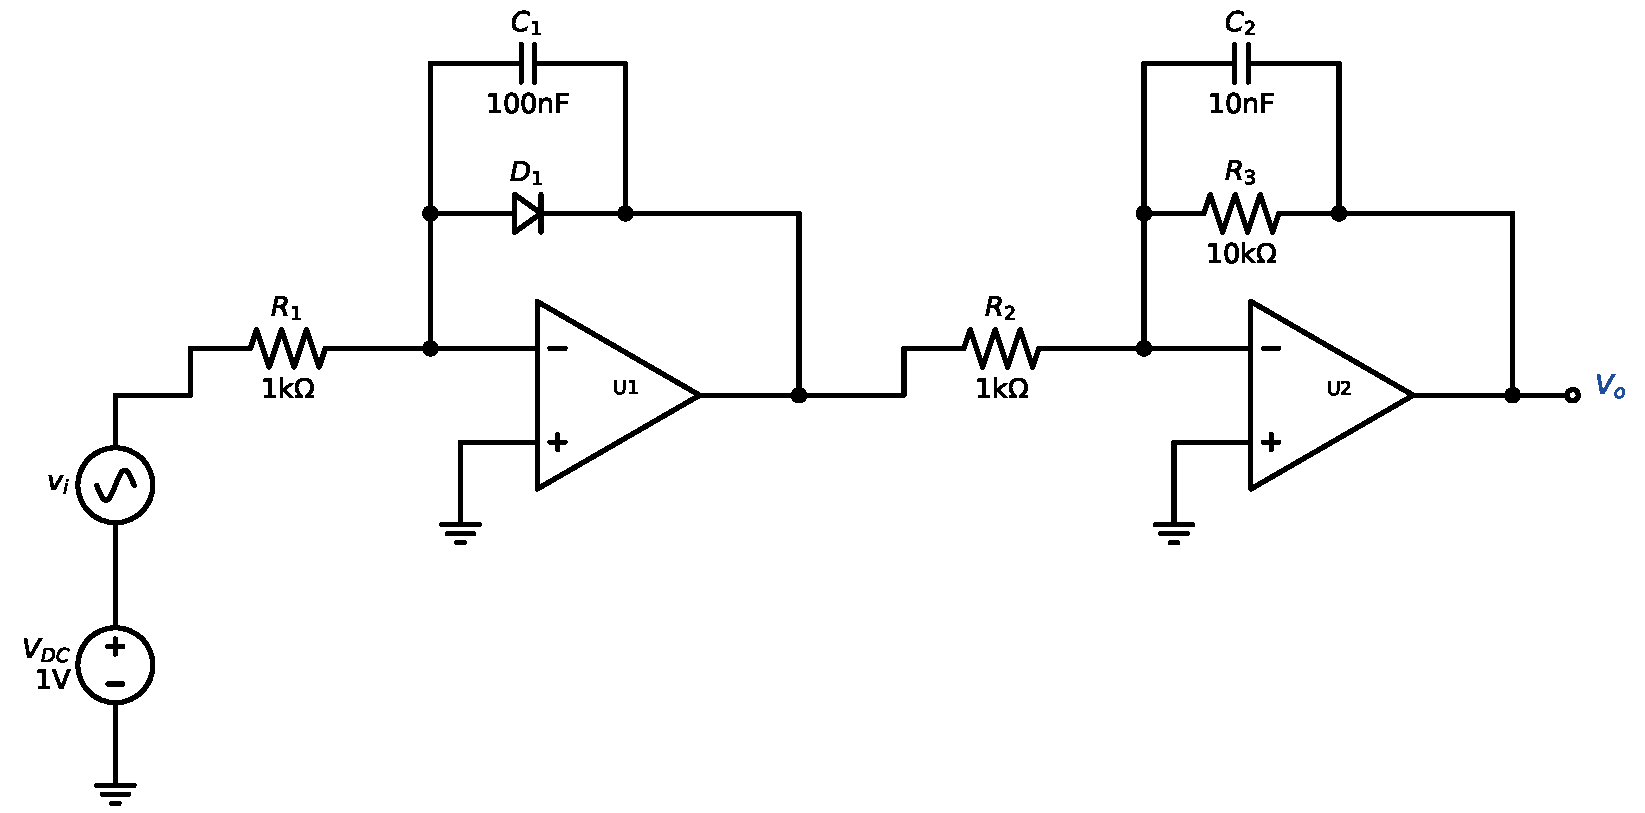
\includegraphics[width=0.9\linewidth,height=5cm,keepaspectratio]{p16_circuit}\end{center}
\solstep{1}{DC operating point}DC rules (tool T3): $v_i = 0$, so the input is just $V_{DC} = 1\,\mathrm{V}$; capacitors are open. The op-amp has negative feedback, so $V_- = V_+ = 0$ (virtual ground) and no current enters its inputs. The input current $\frac{V_{DC} - 0}{R_{1}} = 1\,\mathrm{m}\mathrm{A}$ cannot enter the op-amp: all of it flows through the diode, $I_D = 1\,\mathrm{m}\mathrm{A}$. Exponential model (tool T1):\[
V_D = nV_T\ln\frac{I_D}{I_S} = 1.8\times 0.025\times\ln\frac{0.001}{2.6\times 10^{-9}} = 579\,\mathrm{m}\mathrm{V}
\]
 The diode current flows from the $-$ input (at 0\,V) toward the output, so the output sits $V_D$ below it:\[
V_{o,dc} = -(V_D) = -579\,\mathrm{m}\mathrm{V}
\]
 Block 2 passes DC with its gain at $s=0$, $H_2(0) = -10$: $V_{dc} = -10\times -0.5787 = 5.79\,\mathrm{V}$.\[
\boxed{V_{o,dc} = 5.79\,\mathrm{V}}
\]

\solstep{2}{Small-signal resistance}$r_d = \frac{nV_T}{I_D} = \frac{1.8\times 25\,\mathrm{mV}}{1\,\mathrm{m}\mathrm{A}} = 45\,\Omega$ (tool T3). For the AC analysis the diode is just this resistor, and $V_{DC}$ is replaced by a short (AC ground).
\solstep{3}{AC circuit}\begin{center}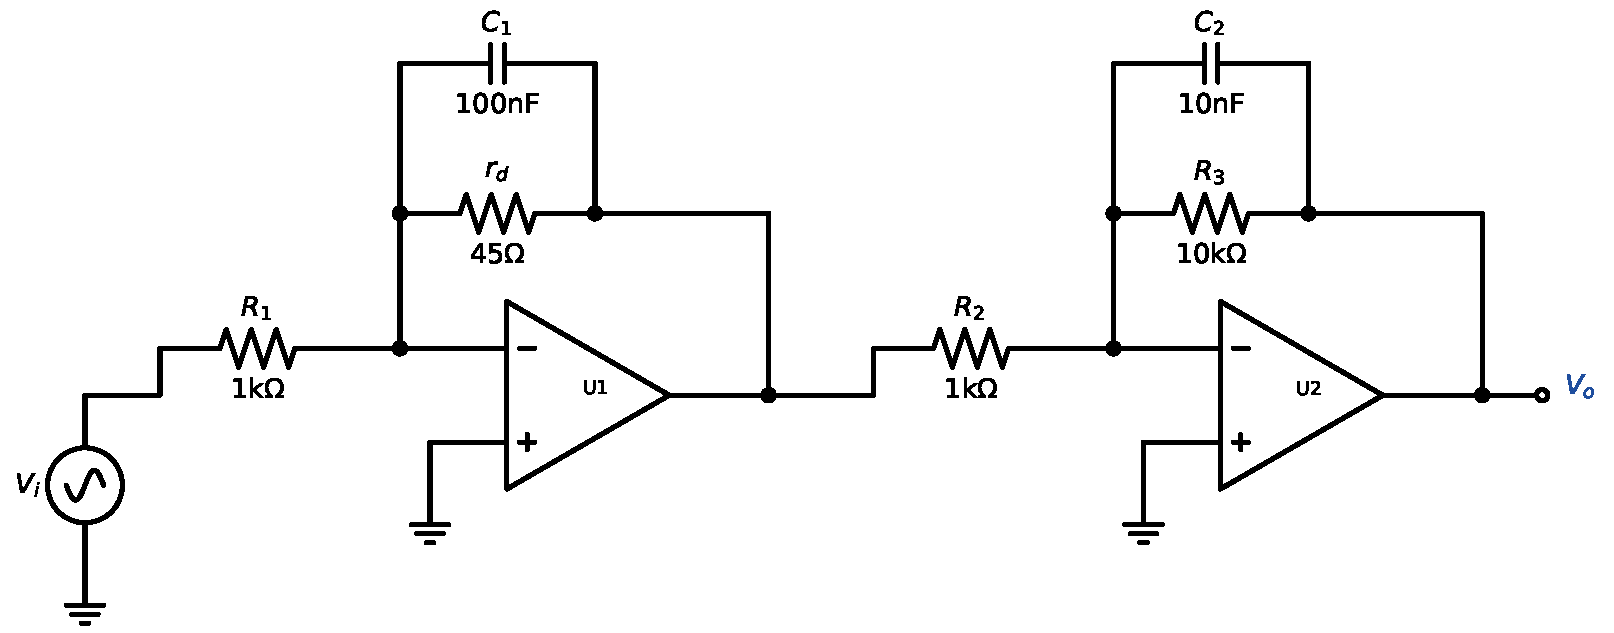
\includegraphics[width=0.9\linewidth,height=5cm,keepaspectratio]{p16_ac}\end{center}

\solstep{4}{Transfer function}Each op-amp output is an ideal voltage source, so a block's output does not change when the next block is connected: the blocks can be solved one at a time and multiplied.\[
H(s) = \frac{V_o}{V_i} = \frac{V_{o1}}{V_{i}}\cdot\frac{V_{o}}{V_{o1}}
\]

\textbf{Block 1 (U1).} Inverting block: the $+$ input is grounded, so $V_- = V_+ = 0$ (virtual ground). The current $\frac{V_{i} - 0}{R_{1}}$ through $R_{1}$ cannot enter the op-amp, so all of it flows through $Z_{f1}$: $V_{o1} = 0 - Z_{f1}\cdot\frac{V_{i}}{R_{1}}$.\begin{align*}
Z_{f1} &= r_d \parallel \frac{1}{sC_{1}} = \dfrac{10^{7}}{s + 2.22\times 10^{5}}
\end{align*}
\[
\frac{V_{o1}}{V_{i}} = -\frac{Z_{f1}}{R_{1}} = \dfrac{-10000}{s + 2.22\times 10^{5}}
\]

\textbf{Block 2 (U2).} Inverting block: the $+$ input is grounded, so $V_- = V_+ = 0$ (virtual ground). The current $\frac{V_{o1} - 0}{R_{2}}$ through $R_{2}$ cannot enter the op-amp, so all of it flows through $Z_{f2}$: $V_{o} = 0 - Z_{f2}\cdot\frac{V_{o1}}{R_{2}}$.\begin{align*}
Z_{f2} &= R_{3} \parallel \frac{1}{sC_{2}} = \dfrac{10^{8}}{s + 10000}
\end{align*}
\[
\frac{V_{o}}{V_{o1}} = -\frac{Z_{f2}}{R_{2}} = \dfrac{-10^{5}}{s + 10000}
\]
Multiply the blocks and simplify:\[
H(s) = \dfrac{10^{9}}{s^{2} + 2.32\times 10^{5}\,s + 2.22\times 10^{9}}
\]

\solstep{5}{Standard (Bode-ready) form}Find the roots. Every root $s=-p$ of the denominator is a \emph{pole}, every root $s=-z$ of the numerator is a \emph{zero}; $|p|$ and $|z|$ are the corner frequencies (rad/s).
\begin{itemize}[leftmargin=*,itemsep=2pt]
\item Denominator: $s^{2} + 2.32\times 10^{5}\,s + 2.22\times 10^{9}$; quadratic formula:\[
s = \frac{-2.32\times 10^{5} \pm \sqrt{(2.32\times 10^{5})^2 - 4(2.22\times 10^{9})}}{2} = \frac{-2.32\times 10^{5} \pm 2.12\times 10^{5}}{2} \Rightarrow s = -10000,\ -2.22\times 10^{5}
\]

\end{itemize}

Factored form (leading coefficient in front):
\[
H(s) = 10^{9}\,\dfrac{1}{(s+10000)(s+2.22\times 10^{5})}
\]

Bode-ready form: rewrite every $(s+p) = p\left(1+\frac{s}{p}\right)$ and $(s+z) = z\left(1+\frac{s}{z}\right)$, and collect all constants into $K$. Then every factor except $K$ is $\approx 1$ inside the pass-band:
\[
H(s) = 0.45\,\dfrac{1}{1+\dfrac{s}{2\pi\cdot 1.59\mathrm{k}}}\,\dfrac{1}{1+\dfrac{s}{2\pi\cdot 35.4\mathrm{k}}},\qquad K = 0.45
\]

\begin{center}\renewcommand{\arraystretch}{1.35}
\begin{tabular}{cccc}
\toprule
type & $\omega_c$ (rad/s) & $f_c=\omega_c/2\pi$ & slope change \\
\midrule
pole & $10000$ & 1.59 kHz & $-20$ dB/dec \\
pole & $2.22\times 10^{5}$ & 35.4 kHz & $-20$ dB/dec \\
\bottomrule
\end{tabular}\end{center}

\solstep{6}{Magnitude Bode plot}Below every corner, all factors are $\approx$ constant: $|H| \approx 0.45$ $= -6.94$\,dB (flat, 0 dB/dec). Then, moving right, each pole bends the line down by 20\,dB/dec and each zero bends it up by 20\,dB/dec (tool T6):
\begin{center}\renewcommand{\arraystretch}{1.35}
\begin{tabular}{lcl}
\toprule
frequency range & slope & asymptote level \\
\midrule
$f<$ 1.59 kHz & $0$ dB/dec (flat) & -6.94 dB at end \\
1.59 kHz -- 35.4 kHz & $-20$ dB/dec & -6.94 dB at start, -33.9 dB at end \\
$f>$ 35.4 kHz & $-40$ dB/dec & -33.9 dB at start \\
\bottomrule
\end{tabular}\end{center}

The flat (pass-band) level is $20\log_{10}|K| = 20\log_{10}0.45 = -6.94$\,dB.
\begin{center}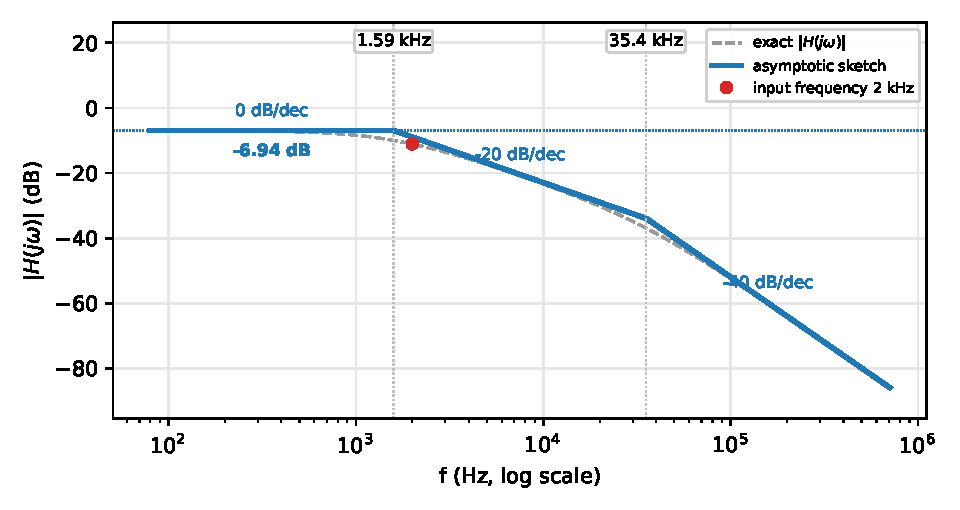
\includegraphics[width=0.78\linewidth,height=6.5cm,keepaspectratio]{p16_bode}\end{center}

{\small Blue: the straight-line sketch you are expected to draw. Dashed grey: the exact curve (about 3\,dB below the corner of an isolated pole). Red dot: the input frequency of Step 7.}
\solstep{7}{Total output (DC + AC)}The input is $V_i(t) = 0.02\sin\left(2\pi\cdot 2000\,t\right)$, so $\omega_{in} = 2\pi\cdot 2000 = 12600$\,rad/s. Put $s=j\omega_{in}$ in each factor (tool T5): magnitudes multiply, angles add.
{\small Rules: $\left|\frac{s}{s+p}\right| = \frac{\omega}{\sqrt{\omega^2+p^2}}$, $\angle = \frac{\pi}{2}-\tan^{-1}\frac{\omega}{p}$;\quad $\left|\frac{1}{1+s/p}\right| = \frac{1}{\sqrt{1+(\omega/p)^2}}$, $\angle = -\tan^{-1}\frac{\omega}{p}$;\quad $\left|1+\frac{s}{z}\right| = \sqrt{1+(\omega/z)^2}$, $\angle = \tan^{-1}\frac{\omega}{z}$;\quad a negative $K$ adds $-\pi$.}
\begin{center}\renewcommand{\arraystretch}{1.35}
\begin{tabular}{ccc}
\toprule
factor & magnitude & angle (rad) \\
\midrule
$0.45$ & $0.45$ & $0$ \\
$\rule[-1.7em]{0pt}{4em}\dfrac{1}{1+\dfrac{s}{2\pi\cdot 1.59\mathrm{k}}}$ & $0.6227$ & $-0.899$ \\
$\rule[-1.7em]{0pt}{4em}\dfrac{1}{1+\dfrac{s}{2\pi\cdot 35.4\mathrm{k}}}$ & $0.9984$ & $-0.0565$ \\
\textbf{total} & $\mathbf{0.2798}$ (product) & $\mathbf{-0.955}$ (sum) \\
\bottomrule
\end{tabular}\end{center}

\begin{align*}
|H(j\omega_{in})| &= 0.28, \qquad \angle H(j\omega_{in}) = -0.955\ \mathrm{rad} \\
v_{o,ac}(t) &= 0.28\times 0.02\,\sin\left(2\pi\cdot 2000\,t - 0.955\right) = 0.0056\,\sin\left(2\pi\cdot 2000\,t - 0.955\right)
\end{align*}

Add the DC part from Step 2 (superposition):
\[
\boxed{V_o(t) = 5.79 + 0.0056\,\sin\left(2\pi\cdot 2000\,t - 0.955\right)\ \mathrm{V}}
\]
 Check the small-signal assumption: the AC voltage across the diode has amplitude about $899\,\mu \mathrm{V}$, well below $nV_T = 45\,\mathrm{m}\mathrm{V}$ \checkmark.
\begin{ansbox}
$H(s) = 0.45\,\dfrac{1}{1+\dfrac{s}{2\pi\cdot 1.59\mathrm{k}}}\,\dfrac{1}{1+\dfrac{s}{2\pi\cdot 35.4\mathrm{k}}}$\quad (corners: 1.59 kHz, 35.4 kHz)\\[4pt]
$V_o(t) = 5.79 + 0.0056\,\sin\left(2\pi\cdot 2000\,t - 0.955\right)\ \mathrm{V}$
\end{ansbox}

\newpage
\subsection*{Solution 3D.17 \hfill Hard}
\begin{center}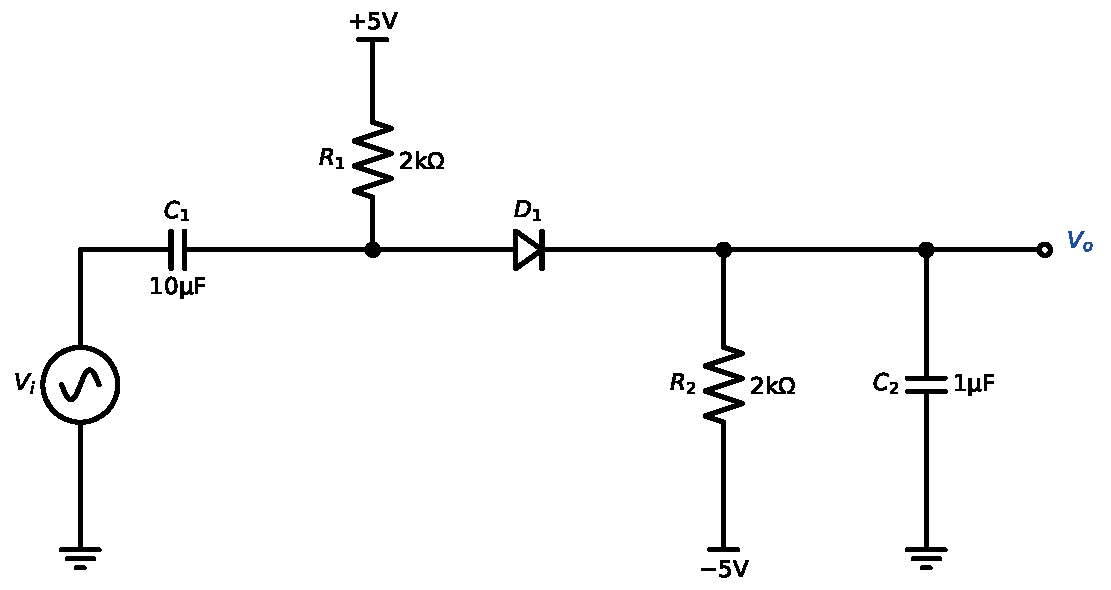
\includegraphics[width=0.9\linewidth,height=5cm,keepaspectratio]{p17_circuit}\end{center}
\solstep{1}{DC operating point}DC rules (tool T3): $v_i = 0$ and every capacitor is open ($C_{1}, C_{2}$). With the exponential model the diode voltage is unknown, so first reduce the rest of the circuit to what the diode sees: a Thevenin source. Remove the diode and solve the circuit (Lecture 2 KCL): the open-circuit voltage across it is $V_{th} = 10\,\mathrm{V}$. Short the diode instead: the current is $I_{sc} = 2.5\,\mathrm{m}\mathrm{A}$. So $R_{th} = \frac{V_{th}}{I_{sc}} = 4\,\mathrm{k}\Omega$.

Two equations, two unknowns: the circuit gives $I_D = \frac{V_{th}-V_D}{R_{th}}$ and the diode gives $V_D = nV_T\ln\frac{I_D}{I_S}$ (tool T1, $n=1.8$, $V_T = 25$\,mV, $I_S = 2.6\,\mathrm{n}\mathrm{A}$). Solve by iteration: guess $V_D = 0.7$\,V, compute $I_D$, update $V_D$, repeat until nothing changes:\begin{center}\renewcommand{\arraystretch}{1.35}
\begin{tabular}{cccc}
\toprule
step & $V_D$ used (V) & circuit $\Rightarrow I_D$ & diode $\Rightarrow$ new $V_D$ (V) \\
\midrule
1 & $0.7$ & $I_D = \frac{10 - 0.7}{4000} = 2.33\,\mathrm{m}\mathrm{A}$ & $0.6167$ \\
2 & $0.6167$ & $I_D = \frac{10 - 0.6167}{4000} = 2.35\,\mathrm{m}\mathrm{A}$ & $0.6171$ \\
3 & $0.6171$ & $I_D = \frac{10 - 0.6171}{4000} = 2.35\,\mathrm{m}\mathrm{A}$ & $0.6171$ \\
4 & $0.6171$ & $I_D = \frac{10 - 0.6171}{4000} = 2.35\,\mathrm{m}\mathrm{A}$ & $0.6171$ \\
5 & $0.6171$ & $I_D = \frac{10 - 0.6171}{4000} = 2.35\,\mathrm{m}\mathrm{A}$ & $0.6171$ \\
\bottomrule
\end{tabular}\end{center}
Converged: $V_D = 0.6171$\,V, $I_D = 2.35\,\mathrm{m}\mathrm{A}$. With this $V_D$ the rest of the DC circuit gives $V_{o,dc} = -309\,\mathrm{m}\mathrm{V}$.\[
\boxed{V_{o,dc} = -309\,\mathrm{m}\mathrm{V}}
\]

\solstep{2}{Small-signal resistance}$r_{d} = \frac{nV_T}{I_D} = \frac{1.8\times 25\,\mathrm{mV}}{2.35\,\mathrm{m}\mathrm{A}} = 19.2\,\Omega$ (tool T3). For the AC analysis the diode is just this resistor.
\solstep{3}{AC circuit}Set every DC supply to zero: each supply rail becomes AC ground. Replace every capacitor by $\frac{1}{sC}$ and every inductor by $sL$.
AC equivalent circuit (nodes named for the next step):
\begin{center}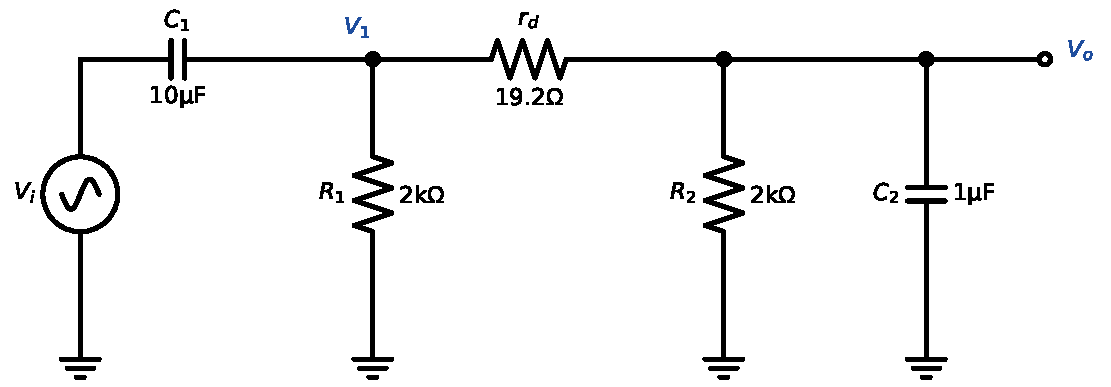
\includegraphics[width=0.95\linewidth,height=5.2cm,keepaspectratio]{p17_ac}\end{center}

\solstep{4}{Transfer function by a chain of dividers}Walk from the input to the output through the named nodes: $V_{i} \to V_{1} \to V_{o}$. The transfer function is the product of the node-to-node ratios (each one is a simple divider, tool T2, or a dependent source, tool T4):
\[
H(s) = \frac{V_o}{V_i} = \frac{V_{1}}{V_{i}}\cdot\frac{V_{o}}{V_{1}}
\]

Impedances seen \emph{looking right} from a node (everything from that node to ground, excluding what is on its left). Compute them from the far right toward the input:
\begin{align*}
Z_{o} &= R_{2} \parallel \frac{1}{sC_{2}} = \dfrac{10^{6}}{s + 500} \\
Z_{1} &= R_{1} \parallel \left(r_d + Z_{o}\right) = \dfrac{19\,s + 10^{6}}{s + 995}
\end{align*}

Now each link. {\small (Algebra tip: to simplify a fraction that contains fractions, multiply its top and bottom by every inner denominator; then divide top and bottom by the leading coefficient of the denominator so that it starts with a plain $s^n$.)}
\begin{align*}
\frac{V_{1}}{V_{i}} &= \frac{Z_{1}}{\frac{1}{sC_{1}} + Z_{1}} = \dfrac{s^{2} + 52600\,s}{s^{2} + 57900\,s + 5.24\times 10^{6}} \\
\frac{V_{o}}{V_{1}} &= \frac{Z_{o}}{r_d + Z_{o}} = \dfrac{52100}{s + 52600}
\end{align*}
Multiply the links and simplify:\[
H(s) = \dfrac{52100\,s}{s^{2} + 57900\,s + 5.24\times 10^{6}}
\]

\solstep{5}{Standard (Bode-ready) form}Find the roots. Every root $s=-p$ of the denominator is a \emph{pole}, every root $s=-z$ of the numerator is a \emph{zero}; $|p|$ and $|z|$ are the corner frequencies (rad/s).
\begin{itemize}[leftmargin=*,itemsep=2pt]
\item Numerator: it has the factor $s$ $\Rightarrow$ 1 zero at $s=0$.
\item Denominator: $s^{2} + 57900\,s + 5.24\times 10^{6}$; quadratic formula:\[
s = \frac{-57900 \pm \sqrt{(57900)^2 - 4(5.24\times 10^{6})}}{2} = \frac{-57900 \pm 57700}{2} \Rightarrow s = -90.6,\ -57800
\]

\end{itemize}

Factored form (leading coefficient in front):
\[
H(s) = 52100\,\dfrac{s}{(s+90.6)(s+57800)}
\]

Bode-ready form: rewrite every $(s+p) = p\left(1+\frac{s}{p}\right)$ and $(s+z) = z\left(1+\frac{s}{z}\right)$, and collect all constants into $K$. Each $s$ in the numerator is paired with one of the \emph{lowest} poles as $\frac{s}{s+p}$ (that factor is $\approx 1$ above $p$). Then every factor except $K$ is $\approx 1$ inside the pass-band:
\[
H(s) = 0.902\,\dfrac{s}{s+2\pi\cdot 14.4}\,\dfrac{1}{1+\dfrac{s}{2\pi\cdot 9.2\mathrm{k}}},\qquad K = 0.902
\]

\begin{center}\renewcommand{\arraystretch}{1.35}
\begin{tabular}{cccc}
\toprule
type & $\omega_c$ (rad/s) & $f_c=\omega_c/2\pi$ & slope change \\
\midrule
pole & $90.6$ & 14.4 Hz & $-20$ dB/dec \\
pole & $57800$ & 9.2 kHz & $-20$ dB/dec \\
\bottomrule
\end{tabular}\end{center}

\solstep{6}{Magnitude Bode plot}Below every corner $|H(s)|\approx 0.00995\,s$, so the plot starts with a slope of $+20$\,dB/dec. Then, moving right, each pole bends the line down by 20\,dB/dec and each zero bends it up by 20\,dB/dec (tool T6):
\begin{center}\renewcommand{\arraystretch}{1.35}
\begin{tabular}{lcl}
\toprule
frequency range & slope & asymptote level \\
\midrule
$f<$ 14.4 Hz & $+20$ dB/dec & -0.897 dB at end \\
14.4 Hz -- 9.2 kHz & $0$ dB/dec (flat) & -0.897 dB at start, -0.897 dB at end \\
$f>$ 9.2 kHz & $-20$ dB/dec & -0.897 dB at start \\
\bottomrule
\end{tabular}\end{center}

The flat (pass-band) level is $20\log_{10}|K| = 20\log_{10}0.902 = -0.897$\,dB.
\begin{center}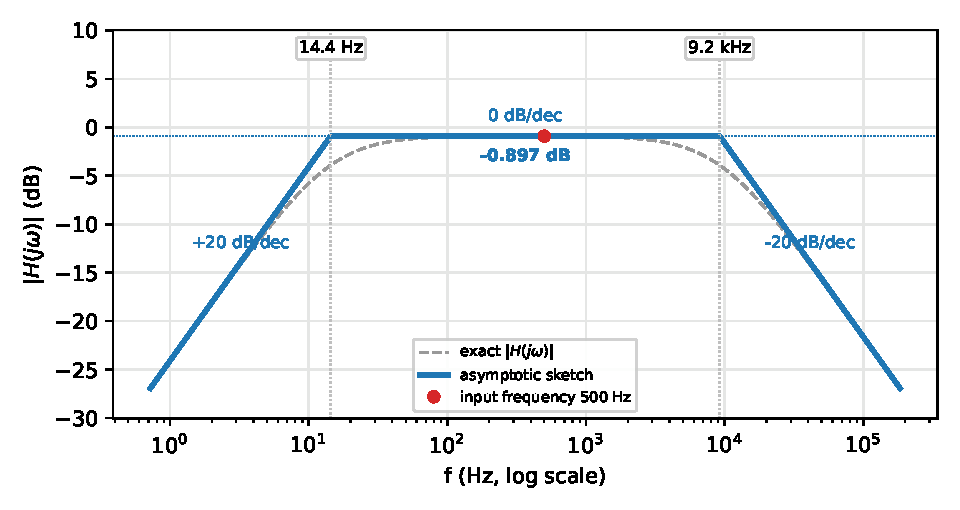
\includegraphics[width=0.78\linewidth,height=6.5cm,keepaspectratio]{p17_bode}\end{center}

{\small Blue: the straight-line sketch you are expected to draw. Dashed grey: the exact curve (about 3\,dB below the corner of an isolated pole). Red dot: the input frequency of Step 7.}
\solstep{7}{Total output (DC + AC)}The input is $V_i(t) = 0.005\sin\left(2\pi\cdot 500\,t\right)$, so $\omega_{in} = 2\pi\cdot 500 = 3140$\,rad/s. Put $s=j\omega_{in}$ in each factor (tool T5): magnitudes multiply, angles add.
{\small Rules: $\left|\frac{s}{s+p}\right| = \frac{\omega}{\sqrt{\omega^2+p^2}}$, $\angle = \frac{\pi}{2}-\tan^{-1}\frac{\omega}{p}$;\quad $\left|\frac{1}{1+s/p}\right| = \frac{1}{\sqrt{1+(\omega/p)^2}}$, $\angle = -\tan^{-1}\frac{\omega}{p}$;\quad $\left|1+\frac{s}{z}\right| = \sqrt{1+(\omega/z)^2}$, $\angle = \tan^{-1}\frac{\omega}{z}$;\quad a negative $K$ adds $-\pi$.}
\begin{center}\renewcommand{\arraystretch}{1.35}
\begin{tabular}{ccc}
\toprule
factor & magnitude & angle (rad) \\
\midrule
$0.902$ & $0.9019$ & $0$ \\
$\rule[-1.1em]{0pt}{2.8em}\dfrac{s}{s+2\pi\cdot 14.4}$ & $0.9996$ & $0.0288$ \\
$\rule[-1.7em]{0pt}{4em}\dfrac{1}{1+\dfrac{s}{2\pi\cdot 9.2\mathrm{k}}}$ & $0.9985$ & $-0.0543$ \\
\textbf{total} & $\mathbf{0.9002}$ (product) & $\mathbf{-0.0255}$ (sum) \\
\bottomrule
\end{tabular}\end{center}

\begin{align*}
|H(j\omega_{in})| &= 0.9, \qquad \angle H(j\omega_{in}) = -0.0255\ \mathrm{rad} \\
v_{o,ac}(t) &= 0.9\times 0.005\,\sin\left(2\pi\cdot 500\,t - 0.0255\right) = 0.0045\,\sin\left(2\pi\cdot 500\,t - 0.0255\right)
\end{align*}

Add the DC part from Step 2 (superposition):
\[
\boxed{V_o(t) = -0.309 + 0.0045\,\sin\left(2\pi\cdot 500\,t - 0.0255\right)\ \mathrm{V}}
\]
 Check the small-signal assumption: the AC voltage across the diode has amplitude about $275\,\mu \mathrm{V}$, well below $nV_T = 45\,\mathrm{m}\mathrm{V}$ \checkmark.
\begin{ansbox}
$H(s) = 0.902\,\dfrac{s}{s+2\pi\cdot 14.4}\,\dfrac{1}{1+\dfrac{s}{2\pi\cdot 9.2\mathrm{k}}}$\quad (corners: 14.4 Hz, 9.2 kHz)\\[4pt]
$V_o(t) = -0.309 + 0.0045\,\sin\left(2\pi\cdot 500\,t - 0.0255\right)\ \mathrm{V}$
\end{ansbox}

\newpage
\subsection*{Solution 3D.18 \hfill Hard}
\begin{center}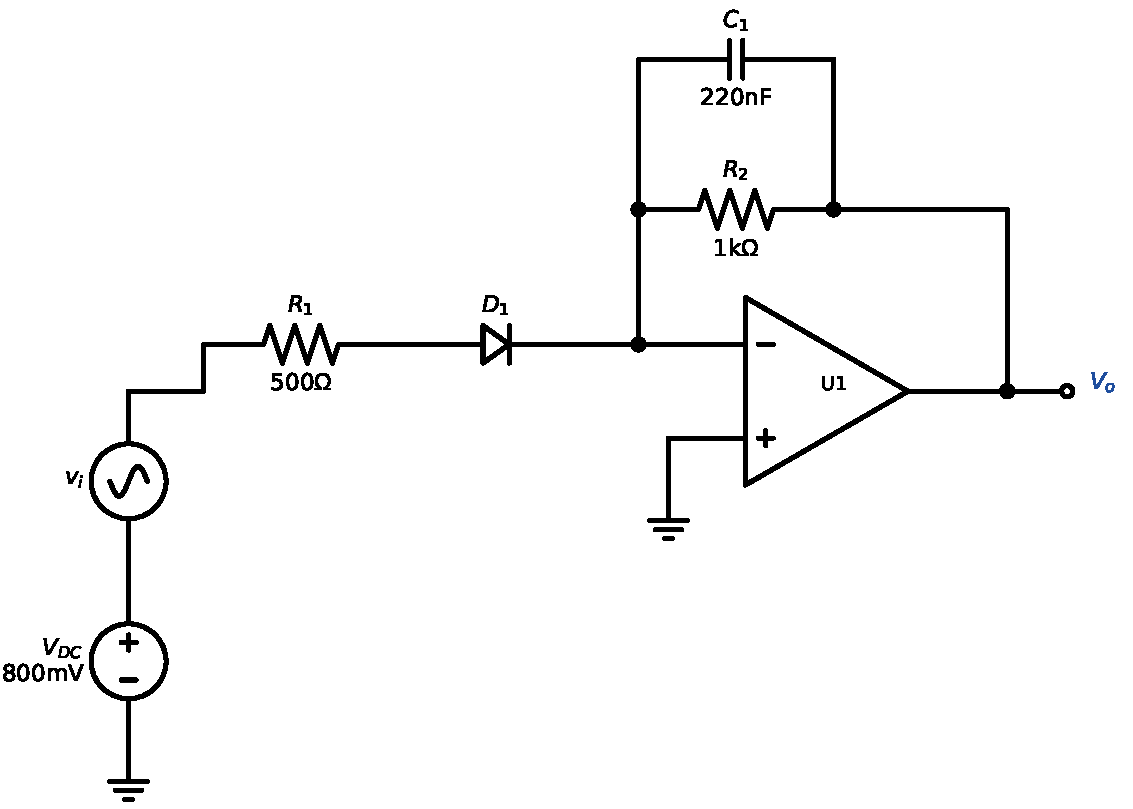
\includegraphics[width=0.9\linewidth,height=5cm,keepaspectratio]{p18_circuit}\end{center}
\solstep{1}{DC operating point}DC rules (tool T3): $v_i = 0$, so the input is just $V_{DC} = 800\,\mathrm{m}\mathrm{V}$; capacitors are open. The op-amp has negative feedback, so $V_- = V_+ = 0$ (virtual ground) and no current enters its inputs. The diode and $R_{1}$ connect $V_{DC}$ to the virtual ground: the diode sees $V_{th} = V_{DC}$ through $R_{th} = R_{1} = 500\,\Omega$.

Two equations, two unknowns: the circuit gives $I_D = \frac{V_{th}-V_D}{R_{th}}$ and the diode gives $V_D = nV_T\ln\frac{I_D}{I_S}$ (tool T1, $n=1$, $V_T = 25$\,mV, $I_S = 1\,\mathrm{p}\mathrm{A}$). Solve by iteration: guess $V_D = 0.7$\,V, compute $I_D$, update $V_D$, repeat until nothing changes:\begin{center}\renewcommand{\arraystretch}{1.35}
\begin{tabular}{cccc}
\toprule
step & $V_D$ used (V) & circuit $\Rightarrow I_D$ & diode $\Rightarrow$ new $V_D$ (V) \\
\midrule
1 & $0.7$ & $I_D = \frac{0.8 - 0.7}{500} = 200\,\mu \mathrm{A}$ & $0.4778$ \\
2 & $0.4778$ & $I_D = \frac{0.8 - 0.4778}{500} = 644\,\mu \mathrm{A}$ & $0.5071$ \\
3 & $0.5071$ & $I_D = \frac{0.8 - 0.5071}{500} = 586\,\mu \mathrm{A}$ & $0.5047$ \\
4 & $0.5047$ & $I_D = \frac{0.8 - 0.5047}{500} = 591\,\mu \mathrm{A}$ & $0.5049$ \\
5 & $0.5049$ & $I_D = \frac{0.8 - 0.5049}{500} = 590\,\mu \mathrm{A}$ & $0.5049$ \\
\bottomrule
\end{tabular}\end{center}
Converged: $I_D = 590\,\mu \mathrm{A}$. All of $I_D$ continues through the feedback resistor $R_{2}$ (the capacitor is open), so\[
V_{o,dc} = 0 - R_{2}I_D = -1000\times5.902\times 10^{-4} = -590\,\mathrm{m}\mathrm{V}
\]
\[
\boxed{V_{o,dc} = -590\,\mathrm{m}\mathrm{V}}
\]

\solstep{2}{Small-signal resistance}$r_d = \frac{nV_T}{I_D} = \frac{1\times 25\,\mathrm{mV}}{590\,\mu \mathrm{A}} = 42.4\,\Omega$ (tool T3). For the AC analysis the diode is just this resistor, and $V_{DC}$ is replaced by a short (AC ground).
\solstep{3}{AC circuit}\begin{center}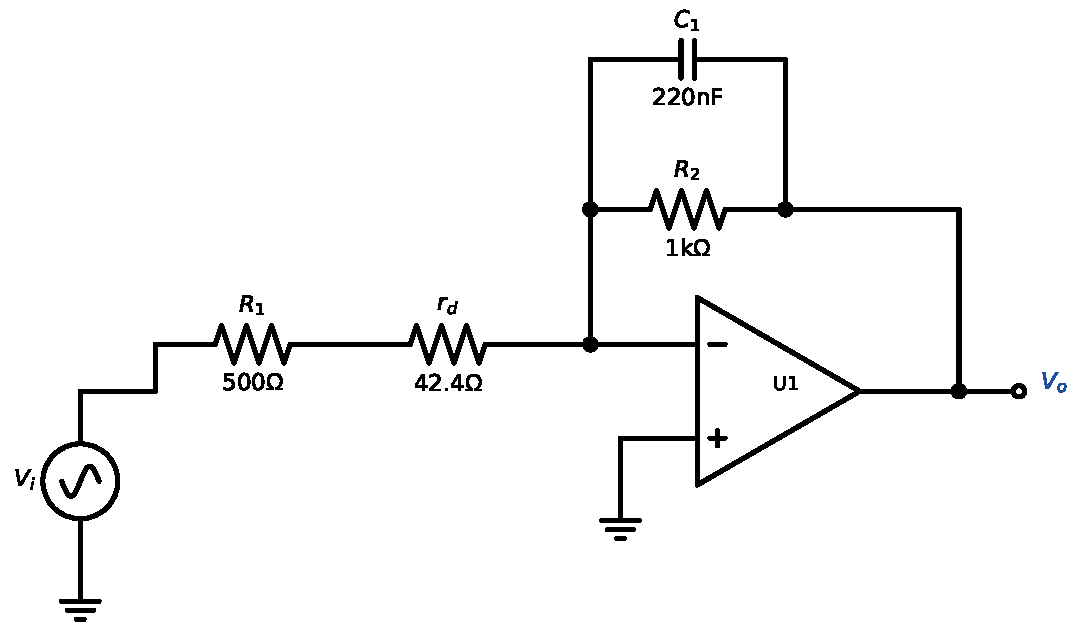
\includegraphics[width=0.9\linewidth,height=5cm,keepaspectratio]{p18_ac}\end{center}

\solstep{4}{Transfer function}\textbf{Block 1 (U1).} Inverting block: the $+$ input is grounded, so $V_- = V_+ = 0$ (virtual ground). The current $\frac{V_{i} - 0}{Z_{in1}}$ through $Z_{in1}$ cannot enter the op-amp, so all of it flows through $Z_{f1}$: $V_{o} = 0 - Z_{f1}\cdot\frac{V_{i}}{Z_{in1}}$.\begin{align*}
Z_{in1} &= R_{1} + r_d = 542 \\
Z_{f1} &= R_{2} \parallel \frac{1}{sC_{1}} = \dfrac{4.55\times 10^{6}}{s + 4550}
\end{align*}
\[
\frac{V_{o}}{V_{i}} = -\frac{Z_{f1}}{Z_{in1}} = \dfrac{-8380}{s + 4550}
\]
So:\[
H(s) = \dfrac{-8380}{s + 4550}
\]

\solstep{5}{Standard (Bode-ready) form}Find the roots. Every root $s=-p$ of the denominator is a \emph{pole}, every root $s=-z$ of the numerator is a \emph{zero}; $|p|$ and $|z|$ are the corner frequencies (rad/s).
\begin{itemize}[leftmargin=*,itemsep=2pt]
\item Denominator: $s + 4550$; $s + 4550 = 0 \Rightarrow s = -4550$.
\end{itemize}

Factored form (leading coefficient in front):
\[
H(s) = -8380\,\dfrac{1}{(s+4550)}
\]

Bode-ready form: rewrite every $(s+p) = p\left(1+\frac{s}{p}\right)$ and $(s+z) = z\left(1+\frac{s}{z}\right)$, and collect all constants into $K$. Then every factor except $K$ is $\approx 1$ inside the pass-band:
\[
H(s) = -1.84\,\dfrac{1}{1+\dfrac{s}{2\pi\cdot 723}},\qquad K = -1.84
\]

\begin{center}\renewcommand{\arraystretch}{1.35}
\begin{tabular}{cccc}
\toprule
type & $\omega_c$ (rad/s) & $f_c=\omega_c/2\pi$ & slope change \\
\midrule
pole & $4550$ & 723 Hz & $-20$ dB/dec \\
\bottomrule
\end{tabular}\end{center}

\solstep{6}{Magnitude Bode plot}Below every corner, all factors are $\approx$ constant: $|H| \approx 1.84$ $= 5.31$\,dB (flat, 0 dB/dec). Then, moving right, each pole bends the line down by 20\,dB/dec and each zero bends it up by 20\,dB/dec (tool T6):
\begin{center}\renewcommand{\arraystretch}{1.35}
\begin{tabular}{lcl}
\toprule
frequency range & slope & asymptote level \\
\midrule
$f<$ 723 Hz & $0$ dB/dec (flat) & 5.31 dB at end \\
$f>$ 723 Hz & $-20$ dB/dec & 5.31 dB at start \\
\bottomrule
\end{tabular}\end{center}

The flat (pass-band) level is $20\log_{10}|K| = 20\log_{10}1.84 = 5.31$\,dB.
\begin{center}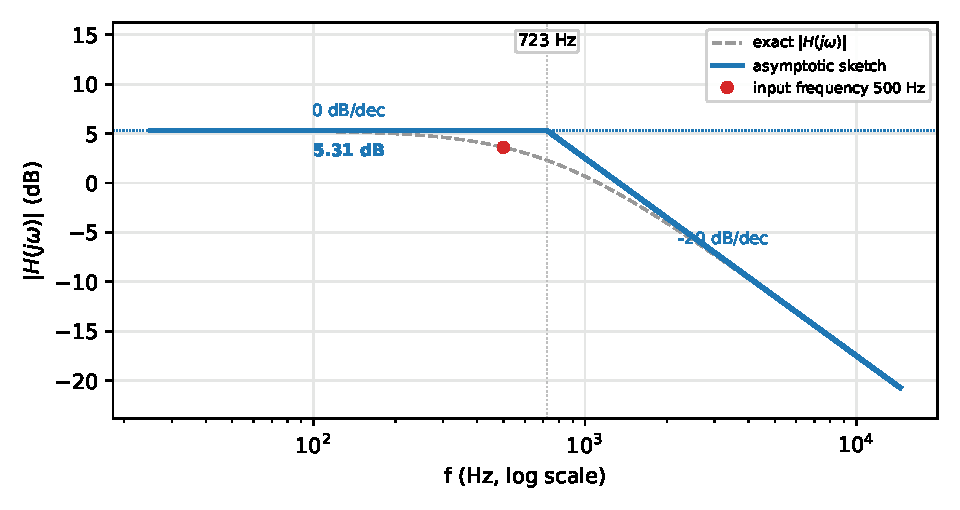
\includegraphics[width=0.78\linewidth,height=6.5cm,keepaspectratio]{p18_bode}\end{center}

{\small Blue: the straight-line sketch you are expected to draw. Dashed grey: the exact curve (about 3\,dB below the corner of an isolated pole). Red dot: the input frequency of Step 7.}
\solstep{7}{Total output (DC + AC)}The input is $V_i(t) = 0.005\cos\left(2\pi\cdot 500\,t-\frac{\pi}{3}\right)$, so $\omega_{in} = 2\pi\cdot 500 = 3140$\,rad/s. Put $s=j\omega_{in}$ in each factor (tool T5): magnitudes multiply, angles add.
{\small Rules: $\left|\frac{s}{s+p}\right| = \frac{\omega}{\sqrt{\omega^2+p^2}}$, $\angle = \frac{\pi}{2}-\tan^{-1}\frac{\omega}{p}$;\quad $\left|\frac{1}{1+s/p}\right| = \frac{1}{\sqrt{1+(\omega/p)^2}}$, $\angle = -\tan^{-1}\frac{\omega}{p}$;\quad $\left|1+\frac{s}{z}\right| = \sqrt{1+(\omega/z)^2}$, $\angle = \tan^{-1}\frac{\omega}{z}$;\quad a negative $K$ adds $-\pi$.}
\begin{center}\renewcommand{\arraystretch}{1.35}
\begin{tabular}{ccc}
\toprule
factor & magnitude & angle (rad) \\
\midrule
$-1.84$ & $1.844$ & $-3.14$ \\
$\rule[-1.7em]{0pt}{4em}\dfrac{1}{1+\dfrac{s}{2\pi\cdot 723}}$ & $0.8226$ & $-0.605$ \\
\textbf{total} & $\mathbf{1.517}$ (product) & $\mathbf{-3.75}$ (sum) \\
\bottomrule
\end{tabular}\end{center}

\begin{align*}
|H(j\omega_{in})| &= 1.52, \qquad \angle H(j\omega_{in}) = -3.75\ \mathrm{rad} \\
v_{o,ac}(t) &= 1.52\times 0.005\,\cos\left(2\pi\cdot 500\,t - 4.79\right) = 0.00758\,\cos\left(2\pi\cdot 500\,t - 4.79\right)
\end{align*}

(phase: $\theta + \angle H = -\frac{\pi}{3} + (-3.75) = -4.79$\,rad.)
Add the DC part from Step 2 (superposition):
\[
\boxed{V_o(t) = -0.59 + 0.00758\,\cos\left(2\pi\cdot 500\,t - 4.79\right)\ \mathrm{V}}
\]
 Check the small-signal assumption: the AC voltage across the diode has amplitude about $391\,\mu \mathrm{V}$, well below $nV_T = 25\,\mathrm{m}\mathrm{V}$ \checkmark.
\begin{ansbox}
$H(s) = -1.84\,\dfrac{1}{1+\dfrac{s}{2\pi\cdot 723}}$\quad (corners: 723 Hz)\\[4pt]
$V_o(t) = -0.59 + 0.00758\,\cos\left(2\pi\cdot 500\,t - 4.79\right)\ \mathrm{V}$
\end{ansbox}

\end{document}
